\documentclass[12pt,a4paper]{article}
\usepackage{amsmath,amssymb,amsthm,amsbsy,amsfonts,mathtools}
\usepackage{url}
\usepackage{hyperref}

\usepackage{listings}
\lstdefinelanguage{julia}{
  basicstyle=\small\ttfamily,
  showspaces=false,
  showstringspaces=false,
  keywordstyle={\textbf},
  morekeywords={if,else,elseif,while,for,begin,end,quote,try,catch,return,local,abstract,function,generated,macro,ccall,finally,typealias,break,continue,type,global,module,using,import,export,const,let,bitstype,do,in,baremodule,importall,immutable},
  escapeinside={~}{~},
  morecomment=[l]{\#},
  commentstyle={},
  morestring=[b]",
}
\lstset{language=julia, numbers=left, numberstyle=\tiny, mathescape=true}

\bibliographystyle{siam}

\usepackage{todonotes}

\author{Yingbo Ma \\ \tt{yingbom@uci.edu}}
\date{March 2018}
\title{Stiffness Detection and Automatic Switching Algorithms for
OrdinaryDiffEq.jl and Tooling for ModelingToolkit.jl \\
\large{Proposal for the GSoC 2018 Project}}

\begin{document}
\maketitle
% \tableofcontents

\begin{abstract}
  Stiff ordinary differential equations (ODEs) and differential algebraic
  equations (DAEs) with high index number are problems present in physical
  models like Brusselator and Euler-Lagrange equations with constraints.
  Stiffness detection and automatic switching algorithms will not only help
  users choose a near optimal solver for the problem, but it will also greatly
  improve the efficiency of solving ODEs by switching algorithms within the
  time domain of interest. Stiffness detection and automatic switching
  algorithms are not presently implemented for most ODE solvers except
  \texttt{LSODA}. Also, there is no open source index reduction algorithm for
  DAEs. Thus, my project aims to implement production ready stiffness detection
  and automatic switching algorithms, and index reduction algorithms for DAEs
  by the end of this summer.
\end{abstract}

\section{Motivation and The Project}
% 1) Very high level overview: why should people who don't know the subject care?
% 2) Dive in, what are the concrete problems you want to solve? Why are they interesting?
% 3) How are you going to solve them? Basically lay out what you're going to write about.
Ordinary differential equations (ODEs) are very important because they arise
from many branches of science. Most of the ODEs which people encounter have no
analytical solution. Hence, people must solve them numerically. Stiff ODEs are
often produced from chemical reaction systems, electrical circuits and
discretization of diffusion partial differential equations (PDEs). Stiff ODEs
cause explicit numerical methods to fail because the ODE system forces them to
have very small time steps. Stiff ODE solvers can avoid this problem by taking
a peek at the next time step. However, this technique comes with a high cost,
which is to solve a linear or non-linear system at each step. People usually do
not know whether their ODE systems are stiff before actually solving them.
Automatic stiffness detection and switching algorithms will enable us to avoid
the hassle of choosing a correction solver for each problem by classifying the
problem type and selecting an appropriate solver automatically.

Differential algebraic equations (DAEs) arise from a wide range of problems
like multi-body and rigid body mechanics, electrical circuit design and optimal
control. Many of those problems come from Euler-Lagrange equations with
constraints. DAEs are not easy to solve because numerical methods are only
specialized for solving their low-index form, however, most of the practical
problems are not in the desired form. Hence, index reduction algorithms can
give a huge productivity boost for people who work on solving DAEs, as index
lowering procedures are not trivial.

For example, I am interested in the Brusselator --- a model that describes a
kind of autocatalysis. It is specified by the reactions
\begin{align*}
  A&\longrightarrow B\\
  2X +  Y&\longrightarrow 3X\\
  B + X&\longrightarrow Y+D\\
  X&\longrightarrow E.
\end{align*}
\begin{wrapfigure}{l}{0.5\textwidth}
  \includegraphics[width=0.5\textwidth]{bz_rect}
  \centering
  \caption{BZ reaction}
\end{wrapfigure}
Thus, we have a PDE system which has the form of
\begin{align}
  \pdv{u}{t} &= A + u^2v - (B+1)u + \alpha \laplacian{u} \\
  \pdv{v}{t} &= Bu - u^2v + \alpha \laplacian{v}.
\end{align}
This problem is interesting, because it can be used to study pattern formation
and chemical clock reactions, e.g. Belousov--Zhabotinsky reaction (BZ
reaction), which is a nonlinear chemical oscillator. \textit{Method of lines}
is a common method for Brusselator, and it leads to a large system of stiff
ODEs. Its stiffness comes from the translation of the diffusion terms
$\laplacian u$ and $\laplacian v$.

Another mathematical model that I am interested in is rigid body dynamics.
Formulating problems in terms of manifold and local coordinates is usually very
cumbersome. One can use Lagrange multipliers to solve those kind of problems
easily, since one can write the problem as normal and only needs to add
holonomic constraints and Lagrange multipliers. For instance, the motion of a
simple pendulum in Cartesian coordinates $(x, y)$ can be described by
\begin{align}
  x'' &= -\lambda x \\
  y'' &= -\lambda y - g \\
  x^2 + y^2 &= 1.
\end{align}
However, this system has a differentiation index of 3. Numerical methods are
not able to solve such a system. Thus, one must use indexing reaction
algorithms to transform the above into a index-1 form.

Hence, there are two projects that I propose for the Google Summer of Code
(GSoC) Program, one is \textit{stiffness detection and automatic switching
algorithms}, and the other is \textit{tooling of} \texttt{ModelingToolkit.jl}.
By the end of the program, I hope to have implemented production ready
automatic stiffness detection algorithms, intermediate representation (IR)
manipulating tools, and index reduction algorithm for differential algebraic
equations.

\subsection{Goal 1: Implement stiffness detection and automatic switching
algorithms} \label{goal1}
An ordinary differential equation (ODE) is an equality relationship among a
function $y(t)$, its independent variable $t$ and its derivatives. An $n$th
order ODE can be written as
\begin{equation}
  F(t, y(t), y'(t), \cdots, y^{(n-1)}(t)) = 0.
\end{equation}
While stiff ODEs are a kind of problem which is very hard to solve by most
explicit numerical methods, they can be solved by implicit methods like the
family of Rosenbrock methods, implicit Runge-Kutta methods or backward
differentiation formulae (BDF) without any issue. The problem is that the
methods which work well for stiff ODEs are not fast, as they have to solve for
non-linear or linear systems in each time step. Yet, most stiff problems are
not stiff throughout the whole domain of interest. This leads to the motivation
of my first project, \textit{stiffness detection and automatic switching
algorithms}. Conventionally, one uses only a single algorithm to solve for the
entire domain of interest. Thus, one is forced to use a stiff algorithm,
although there is only a very small interval in the domain that is stiff. The
auto-switching algorithm can solve this dilemma and raise the efficiency of
solving ODEs, because stiff algorithms will only be applied to the stiff part
of the domain, and non-stiff algorithms will solve the rest of the problem
quickly. This project is beneficial for most people who use the
\textit{JuliaDiffEq} ecosystem, because it removes the burden of having to test
multiple algorithms for one problem and chose the more efficient one. It can
also help to save computation time for ODE systems, e.g. time stepping of a PDE
discretization.

\subsubsection{Implementation Details}
Higham and Trefethen~\cite{stiffode} pointed out that an ODE system is stiff
when the pseudospectrum of its $J$ has large radii while it has a small abscissa,
where $J$ denotes a Jacobian matrix. Computing the pseudospectra of a linear
operator is very costly, so in practice, it makes sense to only calculate the norm
or the approximated largest eigenvalue of $J$.

The simplest automatic stiffness detection on explicit Runge-Kutta algorithms
is proposed by Ernst Hairer~\cite{hairer2}. One can use
\begin{equation}
  \abs{\lambda} = \frac{\norm{f(y+v, t)-f(y, t)}}{\norm{v}}
\end{equation}
to approximate the dominant eigenvalue of the Jacobian matrix of the function
$f(y, t)$ when $\norm{v}$ is small. For explicit Runge-Kutta methods like
Dormand-Prince and Tsitouras $5/4$ pairs, there is the relation $c_6 = c_7 =
1$. Hence, one can use
\begin{equation}
  \varrho = \frac{\norm{k_7-k_6}}{\norm{g_7-k_6}}\qqtext{where } k_i = f(g_i,
  t_0 + c_i\cdot \Delta t)
\end{equation}
to produce a reasonable approximation of the most significant eigenvalue.
Naturally, one can classify a problem to be stiff when $\Delta
t\cdot\varrho/S \ll 1$. Where $S$ is the width of the stability domain of the
Runge-Kutta algorithm. Currently, the implementation reads:

\begin{lstlisting}
g6 = uprev+dt*(a61*k1+a62*k2+a63*k3+a64*k4+a65*k5)
k6 = f(g6, p, t+dt)
g7 = u
rho = integrator.opts.internalnorm(k7 - k6)/
      integrator.opts.internalnorm(g7 - g6)
stiffness = rho*dt/3.3
\end{lstlisting}

Here is a demonstration of this automatic stiffness detection method with the
infamous Dormand-Prince $5/4$ integrator. The ODEs that the integrator solves
are
\begin{align}
  y'_1 &= y_2\\
  y'_2 &= ((1-y_1^2)y_2-y_1) / \varepsilon
\end{align}
where $\varepsilon$ is $0.003$.

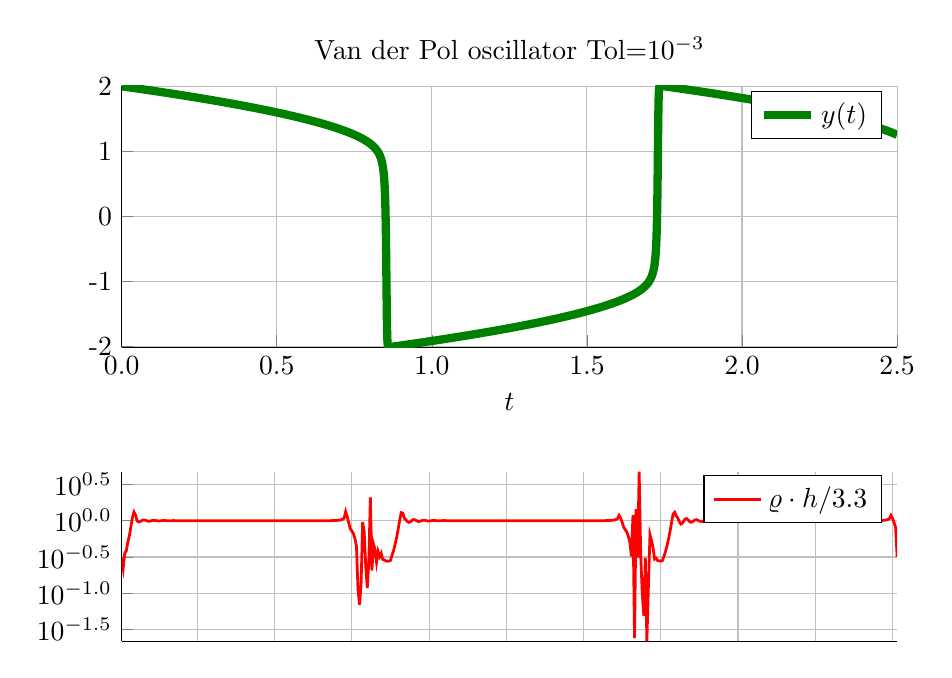
\begin{tikzpicture}[]
\begin{axis}[height = {49.00083333333333mm}, ylabel = {}, title = {Van der Pol oscillator Tol=$10^{-3}$}, xmin = {0.0}, xmax = {2.5}, ymax = {2.0083206559984887}, xlabel = {$t$}, {unbounded coords=jump, scaled x ticks = false, xticklabel style={rotate = 0}, xmajorgrids = true, xtick = {0.0,0.5,1.0,1.5,2.0,2.5}, xticklabels = {0.0,0.5,1.0,1.5,2.0,2.5}, xtick align = inside, axis lines* = left, scaled y ticks = false, yticklabel style={rotate = 0}, ymajorgrids = true, ytick = {-2.0,-1.0,0.0,1.0,2.0}, yticklabels = {-2,-1,0,1,2}, ytick align = inside, axis lines* = left,     xshift = 0.0mm,
    yshift = 37.36mm,
    axis background/.style={fill={rgb,1:red,1.00000000;green,1.00000000;blue,1.00000000}}
}, ymin = {-2.008846245013984}, width = {114.3mm}]\addplot+ [color = {rgb,1:red,0.00000000;green,0.50196078;blue,0.00000000},
draw opacity=1.0,
line width=3,
solid,mark = none,
mark size = 2.0,
mark options = {
    color = {rgb,1:red,0.00000000;green,0.00000000;blue,0.00000000}, draw opacity = 1.0,
    fill = {rgb,1:red,0.00000000;green,0.60560316;blue,0.97868012}, fill opacity = 1.0,
    line width = 1,
    rotate = 0,
    solid
}]coordinates {
(0.0, 2.0)
(0.0005177055290950507, 1.9999247356337337)
(0.0010354110581901014, 1.9997393790039202)
(0.0015531165872851522, 1.9994900063937813)
(0.0020708221163802027, 1.9992020635531769)
(0.0025885276454752537, 1.9988906882352275)
(0.0031062331745703043, 1.9985655024509594)
(0.0036239387036653553, 1.9982322851811072)
(0.0041416442327604054, 1.9978938572049496)
(0.0046593497618554565, 1.9975527250158052)
(0.0051770552909505075, 1.9972096091003322)
(0.0056947608200455585, 1.9968651415186047)
(0.006212466349140609, 1.9965202272278988)
(0.00673017187823566, 1.9961748816520675)
(0.007247877407330711, 1.9958290659752023)
(0.007765582936425761, 1.9954829578816868)
(0.008283288465520811, 1.9951368369389295)
(0.008800993994615862, 1.9947906073044315)
(0.009318699523710913, 1.9944441734166143)
(0.009836405052805964, 1.9940975285276248)
(0.010354110581901015, 1.9937507447099414)
(0.010871816110996066, 1.9934039674686612)
(0.011389521640091117, 1.9930572127113597)
(0.011907227169186166, 1.992710339749901)
(0.012424932698281217, 1.9923632644997127)
(0.012942638227376268, 1.9920159644397426)
(0.01346034375647132, 1.9916684786124588)
(0.01397804928556637, 1.991320907623849)
(0.014495754814661421, 1.990973415945307)
(0.01501346034375647, 1.990626278425988)
(0.015531165872851522, 1.990279193807618)
(0.016048871401946573, 1.989931759025207)
(0.016566576931041622, 1.9895837576672708)
(0.017084282460136675, 1.9892351599758307)
(0.017601987989231724, 1.9888861228464134)
(0.018119693518326777, 1.9885369898280525)
(0.018637399047421826, 1.9881882911232858)
(0.01915510457651688, 1.9878405915131723)
(0.019672810105611928, 1.9874932014694415)
(0.020190515634706977, 1.9871452296970167)
(0.02070822116380203, 1.986796304146016)
(0.02122592669289708, 1.9864465493563135)
(0.021743632221992132, 1.9860965864575382)
(0.02226133775108718, 1.9857475227861423)
(0.022779043280182234, 1.9853993570576511)
(0.023296748809277283, 1.985050913006169)
(0.023814454338372332, 1.984701712526979)
(0.024332159867467385, 1.9843517093356733)
(0.024849865396562434, 1.9840012889681544)
(0.025367570925657487, 1.983651268780634)
(0.025885276454752536, 1.9833022075533062)
(0.02640298198384759, 1.9829530989546973)
(0.02692068751294264, 1.9826034303331586)
(0.027438393042037688, 1.9822530537875471)
(0.02795609857113274, 1.9819021715412974)
(0.02847380410022779, 1.9815513359424222)
(0.028991509629322842, 1.9812013036491851)
(0.029509215158417892, 1.9808515749813165)
(0.03002692068751294, 1.9805014737531899)
(0.030544626216607994, 1.9801507172467103)
(0.031062331745703043, 1.9797993414549055)
(0.03158003727479809, 1.9794477010819247)
(0.032097742803893145, 1.97909646954304)
(0.0326154483329882, 1.9787460526389504)
(0.033133153862083244, 1.9783956076311768)
(0.033650859391178296, 1.9780446071312319)
(0.03416856492027335, 1.9776928671456102)
(0.0346862704493684, 1.9773405437447313)
(0.03520397597846345, 1.9769881330629389)
(0.0357216815075585, 1.9766364581388765)
(0.03623938703665355, 1.976285517753926)
(0.0367570925657486, 1.9759343617409273)
(0.03727479809484365, 1.9755824912503184)
(0.037792503623938704, 1.975229796045869)
(0.03831020915303376, 1.9748765545046805)
(0.0388279146821288, 1.974523433617186)
(0.039345620211223856, 1.9741713616506609)
(0.03986332574031891, 1.9738197953446641)
(0.040381031269413954, 1.9734678092479496)
(0.04089873679850901, 1.9731149946913062)
(0.04141644232760406, 1.9727613613381507)
(0.04193414785669911, 1.972407337184526)
(0.04245185338579416, 1.9720537685591035)
(0.04296955891488921, 1.9717013242883885)
(0.043487264443984264, 1.9713489293945556)
(0.04400496997307931, 1.9709959277595268)
(0.04452267550217436, 1.970642091356466)
(0.045040381031269415, 1.9702875940053428)
(0.04555808656036447, 1.9699330113729325)
(0.046075792089459514, 1.9695792823093707)
(0.046593497618554566, 1.9692261887061735)
(0.04711120314764962, 1.9688727994525712)
(0.047628908676744665, 1.9685187114199947)
(0.04814661420583972, 1.9681638834303021)
(0.04866431973493477, 1.967808636255779)
(0.04918202526402982, 1.9674536526191382)
(0.04969973079312487, 1.967099611740467)
(0.05021743632221992, 1.9667456996334065)
(0.050735141851314974, 1.966391303319024)
(0.05125284738041002, 1.9660361842683933)
(0.05177055290950507, 1.965680438335494)
(0.052288258438600126, 1.965324495757209)
(0.05280596396769518, 1.9649691206916426)
(0.053323669496790224, 1.964614514055357)
(0.05384137502588528, 1.9642597767809609)
(0.05435908055498033, 1.9639044364959009)
(0.054876786084075375, 1.9635483539581076)
(0.05539449161317043, 1.963191723055994)
(0.05591219714226548, 1.9628350708084576)
(0.05642990267136053, 1.962479216905507)
(0.05694760820045558, 1.9621239536391712)
(0.05746531372955063, 1.9617684135927427)
(0.057983019258645685, 1.9614121745081337)
(0.05850072478774073, 1.9610551650047734)
(0.059018430316835784, 1.960697664579609)
(0.059536135845930836, 1.9603403036071043)
(0.06005384137502588, 1.9599839194754414)
(0.060571546904120935, 1.9596279532515248)
(0.06108925243321599, 1.959271584263264)
(0.06160695796231104, 1.9589144435669756)
(0.062124663491406086, 1.958556530079284)
(0.06264236902050115, 1.9581982105771203)
(0.06316007454959618, 1.9578402196977227)
(0.06367778007869124, 1.957483289198844)
(0.06419548560778629, 1.9571265361530532)
(0.06471319113688134, 1.9567692648343953)
(0.0652308966659764, 1.9564111926874583)
(0.06574860219507145, 1.956052404357575)
(0.06626630772416649, 1.955693351690823)
(0.06678401325326154, 1.9553348537340245)
(0.06730171878235659, 1.954977300866042)
(0.06781942431145165, 1.9546196754455616)
(0.0683371298405467, 1.9542614448492819)
(0.06885483536964175, 1.9539024301411576)
(0.0693725408987368, 1.9535428028785355)
(0.06989024642783184, 1.953183085112154)
(0.0704079519569269, 1.9528241291559252)
(0.07092565748602195, 1.9524658353080986)
(0.071443363015117, 1.9521073050285687)
(0.07196106854421205, 1.9517481156483623)
(0.0724787740733071, 1.951388177158245)
(0.07299647960240216, 1.9510277322087217)
(0.0735141851314972, 1.9506673561100352)
(0.07403189066059225, 1.9503078546689427)
(0.0745495961896873, 1.9499487850197335)
(0.07506730171878236, 1.9495893713921764)
(0.07558500724787741, 1.9492292600079253)
(0.07610271277697246, 1.9488684222695005)
(0.07662041830606751, 1.9485071547602877)
(0.07713812383516255, 1.9481460792445375)
(0.0776558293642576, 1.9477859400935116)
(0.07817353489335266, 1.9474260948269246)
(0.07869124042244771, 1.9470658330667552)
(0.07920894595154276, 1.9467048371586173)
(0.07972665148063782, 1.9463431182449873)
(0.08024435700973287, 1.9459810162652031)
(0.08076206253882791, 1.9456191999554655)
(0.08127976806792296, 1.9452583663433503)
(0.08179747359701801, 1.9448977402122667)
(0.08231517912611307, 1.9445366444692702)
(0.08283288465520812, 1.9441747841709753)
(0.08335059018430317, 1.9438122002573492)
(0.08386829571339822, 1.943449269551712)
(0.08438600124249326, 1.943086704760736)
(0.08490370677158832, 1.9427251445477283)
(0.08542141230068337, 1.9423637112265981)
(0.08593911782977842, 1.9420017668900444)
(0.08645682335887347, 1.9416390435200197)
(0.08697452888796853, 1.9412756105346667)
(0.08749223441706358, 1.9409118747883174)
(0.08800993994615862, 1.940548580571494)
(0.08852764547525367, 1.9401862670569165)
(0.08904535100434872, 1.939823993285198)
(0.08956305653344378, 1.939461177349616)
(0.09008076206253883, 1.9390975854481853)
(0.09059846759163388, 1.9387333144875876)
(0.09111617312072894, 1.9383687920831723)
(0.09163387864982397, 1.9380047765589563)
(0.09215158417891903, 1.9376416795787617)
(0.09266928970801408, 1.9372785488349562)
(0.09318699523710913, 1.9369148554062843)
(0.09370470076620419, 1.9365503966205786)
(0.09422240629529924, 1.9361852902605914)
(0.09474011182439429, 1.935819974563996)
(0.09525781735348933, 1.9354552082233856)
(0.09577552288258438, 1.9350913025374312)
(0.09629322841167944, 1.9347273227522417)
(0.09681093394077449, 1.9343627689250615)
(0.09732863946986954, 1.9339974553880708)
(0.0978463449989646, 1.9336315095431285)
(0.09836405052805965, 1.9332653718617745)
(0.09888175605715468, 1.9328997958852279)
(0.09939946158624974, 1.9325350659756393)
(0.09991716711534479, 1.9321702566912649)
(0.10043487264443984, 1.931804870171811)
(0.1009525781735349, 1.9314387202444667)
(0.10147028370262995, 1.9310719318429959)
(0.101987989231725, 1.9307049410077348)
(0.10250569476082004, 1.9303384948855942)
(0.10302340028991509, 1.9299729244091297)
(0.10354110581901015, 1.9296072978412524)
(0.1040588113481052, 1.9292411007283292)
(0.10457651687720025, 1.9288741329404118)
(0.1050942224062953, 1.928506506737278)
(0.10561192793539036, 1.9281386467684336)
(0.1061296334644854, 1.9277712900731103)
(0.10664733899358045, 1.9274048539575181)
(0.1071650445226755, 1.927038405443312)
(0.10768275005177055, 1.926671404799335)
(0.1082004555808656, 1.9263036318029394)
(0.10871816110996066, 1.925935178903538)
(0.10923586663905571, 1.925566451222603)
(0.10975357216815075, 1.9251981665536668)
(0.1102712776972458, 1.9248308351382122)
(0.11078898322634086, 1.9244635486174453)
(0.11130668875543591, 1.9240957395663325)
(0.11182439428453096, 1.9237271664572029)
(0.11234209981362601, 1.9233578971390204)
(0.11285980534272105, 1.9229883088373831)
(0.1133775108718161, 1.922619088154524)
(0.11389521640091116, 1.9222508315250018)
(0.11441292193000621, 1.921882691895835)
(0.11493062745910126, 1.9215140694603274)
(0.11544833298819632, 1.9211446991890193)
(0.11596603851729137, 1.9207746194477795)
(0.11648374404638641, 1.9204041719978049)
(0.11700144957548146, 1.9200340019956201)
(0.11751915510457651, 1.9196647856492992)
(0.11803686063367157, 1.9192957844290148)
(0.11855456616276662, 1.9189263519602744)
(0.11907227169186167, 1.9185561924865164)
(0.11958997722095673, 1.9181853078271032)
(0.12010768275005176, 1.9178139973773205)
(0.12062538827914682, 1.9174428581083776)
(0.12114309380824187, 1.9170726349369014)
(0.12166079933733692, 1.9167027642294043)
(0.12217850486643198, 1.9163325309585606)
(0.12269621039552703, 1.9159615971020778)
(0.12321391592462208, 1.9155899185942442)
(0.12373162145371712, 1.9152177453259294)
(0.12424932698281217, 1.9148456211445835)
(0.12476703251190722, 1.9144743305256402)
(0.1252847380410023, 1.9141035713900565)
(0.12580244357009732, 1.913732542011503)
(0.12632014909919237, 1.913360850210119)
(0.12683785462828742, 1.9129883961948322)
(0.12735556015738247, 1.9126153725633601)
(0.12787326568647753, 1.9122422643022094)
(0.12839097121557258, 1.9118698445013471)
(0.12890867674466763, 1.9114981594807363)
(0.12942638227376269, 1.9111263241435448)
(0.12994408780285774, 1.9107538838501814)
(0.1304617933319528, 1.9103806751194279)
(0.13097949886104784, 1.91000682562844)
(0.1314972043901429, 1.9096327542127465)
(0.13201490991923795, 1.9092591708662503)
(0.13253261544833297, 1.9088864959228242)
(0.13305032097742803, 1.9085138276424818)
(0.13356802650652308, 1.9081406360774456)
(0.13408573203561813, 1.90776668901928)
(0.13460343756471319, 1.907392042918131)
(0.13512114309380824, 1.907017042882726)
(0.1356388486229033, 1.9066423226803735)
(0.13615655415199834, 1.906268551044618)
(0.1366742596810934, 1.9058950097131548)
(0.13719196521018845, 1.9055210533613933)
(0.1377096707392835, 1.9051463775004815)
(0.13822737626837855, 1.9047709622968723)
(0.1387450817974736, 1.904395072572323)
(0.13926278732656866, 1.904019257803896)
(0.13978049285566368, 1.903644289757733)
(0.14029819838475874, 1.9032698243828272)
(0.1408159039138538, 1.902895082546963)
(0.14133360944294884, 1.9025196827051338)
(0.1418513149720439, 1.9021435234876203)
(0.14236902050113895, 1.901766783699991)
(0.142886726030234, 1.9013899223231017)
(0.14340443155932905, 1.90101367842413)
(0.1439221370884241, 1.9006382210889596)
(0.14443984261751916, 1.900262663878001)
(0.1449575481466142, 1.8998865407688001)
(0.14547525367570927, 1.899509662127631)
(0.14599295920480432, 1.8991321147094955)
(0.14651066473389937, 1.8987542616581232)
(0.1470283702629944, 1.898376742505971)
(0.14754607579208945, 1.8980001562157345)
(0.1480637813211845, 1.8976237350209568)
(0.14858148685027955, 1.8972468793525608)
(0.1490991923793746, 1.8968693033860773)
(0.14961689790846966, 1.896490994949843)
(0.1501346034375647, 1.8961122155249985)
(0.15065230896665976, 1.8957335002454905)
(0.15117001449575482, 1.8953556083722796)
(0.15168772002484987, 1.894978244107491)
(0.15220542555394492, 1.8946006257575352)
(0.15272313108303998, 1.894222363857491)
(0.15324083661213503, 1.8938433403656516)
(0.15375854214123008, 1.8934637086635229)
(0.1542762476703251, 1.8930838935558245)
(0.15479395319942016, 1.89270459127049)
(0.1553116587285152, 1.8923261611092708)
(0.15582936425761026, 1.891947719404554)
(0.15634706978670532, 1.8915687617986077)
(0.15686477531580037, 1.8911890586173314)
(0.15738248084489542, 1.8908086490691554)
(0.15790018637399048, 1.890427841245039)
(0.15841789190308553, 1.8900472121184717)
(0.15893559743218058, 1.889667479742169)
(0.15945330296127563, 1.8892881183279164)
(0.1599710084903707, 1.888908426678208)
(0.16048871401946574, 1.888528059168432)
(0.1610064195485608, 1.888146935821691)
(0.16152412507765582, 1.8877652423088032)
(0.16204183060675087, 1.8873834299483012)
(0.16255953613584592, 1.8870022157064323)
(0.16307724166494098, 1.8866217982432192)
(0.16359494719403603, 1.8862413011363028)
(0.16411265272313108, 1.8858602587302167)
(0.16463035825222613, 1.88547846742046)
(0.16514806378132119, 1.8850959855825007)
(0.16566576931041624, 1.884713133571774)
(0.1661834748395113, 1.8843304937236833)
(0.16670118036860634, 1.8839487549008176)
(0.1672188858977014, 1.8835673406743136)
(0.16773659142679645, 1.8831855810285092)
(0.1682542969558915, 1.882803143758397)
(0.16877200248498653, 1.8824199550881018)
(0.16928970801408158, 1.8820361996708816)
(0.16980741354317663, 1.8816523205891273)
(0.17032511907227169, 1.8812690193543624)
(0.17084282460136674, 1.8808865219747686)
(0.1713605301304618, 1.880503960132626)
(0.17187823565955684, 1.8801208665882734)
(0.1723959411886519, 1.8797370299337073)
(0.17291364671774695, 1.8793524940916875)
(0.173431352246842, 1.8789675583157353)
(0.17394905777593705, 1.8785827771901342)
(0.1744667633050321, 1.8781988620932253)
(0.17498446883412716, 1.877815354439676)
(0.17550217436322219, 1.8774315479014263)
(0.17601987989231724, 1.877047087670039)
(0.1765375854214123, 1.8766618715290961)
(0.17705529095050734, 1.8762760498541982)
(0.1775729964796024, 1.8758900256129634)
(0.17809070200869745, 1.8755044543650286)
(0.1786084075377925, 1.8751197672925564)
(0.17912611306688755, 1.8747351277473423)
(0.1796438185959826, 1.874350017578101)
(0.18016152412507766, 1.8739641833440572)
(0.1806792296541727, 1.8735776214671125)
(0.18119693518326777, 1.8731905782318443)
(0.18171464071236282, 1.8728035497855056)
(0.18223234624145787, 1.8724172647689707)
(0.1827500517705529, 1.872031593595791)
(0.18326775729964795, 1.8716457397748127)
(0.183785462828743, 1.871259294472503)
(0.18430316835783805, 1.8708720957249592)
(0.1848208738869331, 1.87048422843791)
(0.18533857941602816, 1.8700960243867153)
(0.1858562849451232, 1.8697080622163664)
(0.18637399047421827, 1.8693209955038328)
(0.18689169600331332, 1.8689342221023975)
(0.18740940153240837, 1.868547101601725)
(0.18792710706150342, 1.8681593098856366)
(0.18844481259059848, 1.867770766454281)
(0.18896251811969353, 1.867381634424135)
(0.18948022364878858, 1.8669923205280017)
(0.1899979291778836, 1.866603475115013)
(0.19051563470697866, 1.8662154954760093)
(0.1910333402360737, 1.8658275485833027)
(0.19155104576516876, 1.8654391323067134)
(0.19206875129426382, 1.8650499969541547)
(0.19258645682335887, 1.8646601331506003)
(0.19310416235245392, 1.8642697718380836)
(0.19362186788154898, 1.8638793842756995)
(0.19413957341064403, 1.8634896770842297)
(0.19465727893973908, 1.8631006455560692)
(0.19517498446883413, 1.8627114791107948)
(0.1956926899979292, 1.8623217547709718)
(0.19621039552702424, 1.8619312867376199)
(0.1967281010561193, 1.8615401263902123)
(0.19724580658521432, 1.8611485622866768)
(0.19776351211430937, 1.8607571201633948)
(0.19828121764340442, 1.8603664995527236)
(0.19879892317249948, 1.8599763396736777)
(0.19931662870159453, 1.8595859259387342)
(0.19983433423068958, 1.8591948919431625)
(0.20035203975978463, 1.8588031055203402)
(0.2008697452888797, 1.8584106687417536)
(0.20138745081797474, 1.8580179179169976)
(0.2019051563470698, 1.8576254235937757)
(0.20242286187616484, 1.8572338133412036)
(0.2029405674052599, 1.8568424800964518)
(0.20345827293435495, 1.8564508036764389)
(0.20397597846345, 1.8560584644380125)
(0.20449368399254503, 1.8556653741119968)
(0.20501138952164008, 1.8552716758031924)
(0.20552909505073513, 1.8548777439903745)
(0.20604680057983019, 1.8544841845262958)
(0.20656450610892524, 1.854091510737222)
(0.2070822116380203, 1.8536989728879538)
(0.20759991716711534, 1.8533060265558365)
(0.2081176226962104, 1.8529123896447033)
(0.20863532822530545, 1.852518008495599)
(0.2091530337544005, 1.8521230578867818)
(0.20967073928349556, 1.8517279410337208)
(0.2101884448125906, 1.8513332895890984)
(0.21070615034168566, 1.8509394882866295)
(0.2112238558707807, 1.8505457245573236)
(0.21174156139987574, 1.8501515067906795)
(0.2122592669289708, 1.8497565815030634)
(0.21277697245806584, 1.8493609205869097)
(0.2132946779871609, 1.848964721310719)
(0.21381238351625595, 1.8485684063190586)
(0.214330089045351, 1.8481726236325635)
(0.21484779457444605, 1.8477776436444426)
(0.2153655001035411, 1.8473826400561637)
(0.21588320563263616, 1.8469871534826294)
(0.2164009111617312, 1.8465909501334927)
(0.21691861669082627, 1.846194018473088)
(0.21743632221992132, 1.8457965692204317)
(0.21795402774901637, 1.8453990353492216)
(0.21847173327811142, 1.845002072087837)
(0.21898943880720645, 1.8446058742616465)
(0.2195071443363015, 1.84420962176165)
(0.22002484986539655, 1.8438128717675553)
(0.2205425553944916, 1.8434154012348387)
(0.22106026092358666, 1.8430172062945736)
(0.2215779664526817, 1.8426185022534305)
(0.22209567198177677, 1.8422197235936766)
(0.22261337751087182, 1.8418215239731761)
(0.22313108303996687, 1.8414240770962125)
(0.22364878856906192, 1.8410265690686523)
(0.22416649409815698, 1.8406285622955092)
(0.22468419962725203, 1.8402298356410753)
(0.22520190515634708, 1.8398303841594827)
(0.2257196106854421, 1.8394304190947026)
(0.22623731621453716, 1.839030367880546)
(0.2267550217436322, 1.8386308741406638)
(0.22727272727272727, 1.838232148576231)
(0.22779043280182232, 1.8378333783298786)
(0.22830813833091737, 1.8374341211657756)
(0.22882584386001242, 1.837034149304217)
(0.22934354938910748, 1.8366334482341184)
(0.22986125491820253, 1.8362322167130185)
(0.23037896044729758, 1.8358308667670766)
(0.23089666597639263, 1.8354300236910743)
(0.2314143715054877, 1.835029984461791)
(0.23193207703458274, 1.8346299429218613)
(0.2324497825636778, 1.834229440158287)
(0.23296748809277282, 1.8338282335623564)
(0.23348519362186787, 1.833426290869884)
(0.23400289915096292, 1.83302379016121)
(0.23452060468005798, 1.832621119861202)
(0.23503831020915303, 1.8322188787392522)
(0.23555601573824808, 1.8318174797254323)
(0.23607372126734313, 1.831416153297968)
(0.2365914267964382, 1.8310144069199146)
(0.23710913232553324, 1.8306119752947758)
(0.2376268378546283, 1.8302088004997519)
(0.23814454338372334, 1.8298050319857369)
(0.2386622489128184, 1.8294010265773208)
(0.23917995444191345, 1.8289973484727884)
(0.2396976599710085, 1.8285945289496466)
(0.24021536550010353, 1.8281918971718445)
(0.24073307102919858, 1.827788904960113)
(0.24125077655829363, 1.8273852566849473)
(0.2417684820873887, 1.8269808610819434)
(0.24228618761648374, 1.8265758312517986)
(0.2428038931455788, 1.826170484660312)
(0.24332159867467384, 1.8257653431383842)
(0.2438393042037689, 1.825361027850434)
(0.24435700973286395, 1.8249570603016685)
(0.244874715261959, 1.824552813757337)
(0.24539242079105406, 1.8241479547330843)
(0.2459101263201491, 1.8237423511058024)
(0.24642783184924416, 1.823336072113631)
(0.2469455373783392, 1.8229293883559574)
(0.24746324290743424, 1.8225227717934167)
(0.2479809484365293, 1.8221168762705695)
(0.24849865396562434, 1.8217115283919145)
(0.2490163594947194, 1.8213060095691234)
(0.24953406502381445, 1.8208999410627904)
(0.2500517705529095, 1.820493142530332)
(0.2505694760820046, 1.8200856320259866)
(0.2510871816110996, 1.8196776260008154)
(0.25160488714019463, 1.8192695393027012)
(0.2521225926692897, 1.8188619851763492)
(0.25264029819838474, 1.8184551903317534)
(0.2531580037274798, 1.8180483674200234)
(0.25367570925657484, 1.8176410826348848)
(0.2541934147856699, 1.817233100257457)
(0.25471112031476495, 1.8168243800420338)
(0.25522882584386003, 1.81641507721608)
(0.25574653137295505, 1.8160055424802342)
(0.25626423690205014, 1.815596322008307)
(0.25678194243114516, 1.8151879426825384)
(0.25729964796024024, 1.8147797643823003)
(0.25781735348933527, 1.8143712436975319)
(0.2583350590184303, 1.813962082648637)
(0.25885276454752537, 1.813552175821057)
(0.2593704700766204, 1.8131416103652727)
(0.2598881756057155, 1.8127306659968017)
(0.2604058811348105, 1.8123198149962005)
(0.2609235866639056, 1.811909695430257)
(0.2614412921930006, 1.8115000841125635)
(0.2619589977220957, 1.8110902890045333)
(0.2624767032511907, 1.8106799432866738)
(0.2629944087802858, 1.810268869786202)
(0.2635121143093808, 1.8098570809770456)
(0.2640298198384759, 1.8094447789798416)
(0.2645475253675709, 1.8090323555619376)
(0.26506523089666595, 1.8086203921373913)
(0.26558293642576103, 1.8082092229523496)
(0.26610064195485605, 1.807798088435705)
(0.26661834748395113, 1.8073865340691873)
(0.26713605301304616, 1.806974304601675)
(0.26765375854214124, 1.8065613314945168)
(0.26817146407123627, 1.8061477329215296)
(0.26868916960033135, 1.8057338137690007)
(0.26920687512942637, 1.8053200656356865)
(0.26972458065852145, 1.8049070985081432)
(0.2702422861876165, 1.8044945236862595)
(0.27075999171671156, 1.8040817100712732)
(0.2712776972458066, 1.803668318237947)
(0.27179540277490166, 1.8032541925375194)
(0.2723131083039967, 1.8028393610977056)
(0.2728308138330917, 1.802424035822696)
(0.2733485193621868, 1.8020086123931576)
(0.2738662248912818, 1.8015936702662332)
(0.2743839304203769, 1.801179498173734)
(0.2749016359494719, 1.8007653371776358)
(0.275419341478567, 1.8003507494067386)
(0.27593704700766203, 1.7999354862124068)
(0.2764547525367571, 1.7995194798029834)
(0.27697245806585213, 1.7991028432437894)
(0.2774901635949472, 1.7986858704571242)
(0.27800786912404224, 1.7982690362222649)
(0.2785255746531373, 1.797852951247699)
(0.27904328018223234, 1.7974373036913576)
(0.27956098571132737, 1.7970214465725858)
(0.28007869124042245, 1.7966050325625258)
(0.2805963967695175, 1.7961878922933145)
(0.28111410229861256, 1.795770034358083)
(0.2816318078277076, 1.7953516453109564)
(0.28214951335680266, 1.7949330896670546)
(0.2826672188858977, 1.7945149099024917)
(0.28318492441499277, 1.7940975367945944)
(0.2837026299440878, 1.7936802816410191)
(0.2842203354731829, 1.7932626604129185)
(0.2847380410022779, 1.792844396750469)
(0.285255746531373, 1.7924253893752968)
(0.285773452060468, 1.7920057120904787)
(0.2862911575895631, 1.7915856137805408)
(0.2868088631186581, 1.7911655184114599)
(0.28732656864775313, 1.7907460243813673)
(0.2878442741768482, 1.790327169015103)
(0.28836197970594324, 1.7899082235247321)
(0.2888796852350383, 1.7894887994197197)
(0.28939739076413334, 1.7890686804156335)
(0.2899150962932284, 1.7886478224341438)
(0.29043280182232345, 1.788226353603023)
(0.29095050735141853, 1.7878045742561466)
(0.29146821288051356, 1.7873829569334916)
(0.29198591840960864, 1.7869620906914072)
(0.29250362393870366, 1.7865416227323228)
(0.29302132946779874, 1.7861209336986215)
(0.29353903499689377, 1.7856996874463766)
(0.2940567405259888, 1.7852777171601095)
(0.29457444605508387, 1.7848550253527888)
(0.2950921515841789, 1.7844317838658315)
(0.295609857113274, 1.7840083338691028)
(0.296127562642369, 1.7835851858609155)
(0.2966452681714641, 1.7831628351246036)
(0.2971629737005591, 1.7827406860737247)
(0.2976806792296542, 1.7823182209491615)
(0.2981983847587492, 1.7818951456115217)
(0.2987160902878443, 1.7814713323729547)
(0.2992337958169393, 1.7810468199971503)
(0.2997515013460344, 1.7806218136993404)
(0.3002692068751294, 1.7801966851462974)
(0.3007869124042245, 1.7797719724563354)
(0.30130461793331953, 1.7793480304672755)
(0.30182232346241455, 1.7789241526505302)
(0.30234002899150964, 1.7784998927947049)
(0.30285773452060466, 1.7780749886790406)
(0.30337544004969974, 1.777649341666151)
(0.30389314557879477, 1.777223016702023)
(0.30441085110788985, 1.776796242316017)
(0.30492855663698487, 1.7763694106208663)
(0.30544626216607995, 1.775943077312677)
(0.305963967695175, 1.7755174562832505)
(0.30648167322427006, 1.7750918161339169)
(0.3069993787533651, 1.7746657517322892)
(0.30751708428246016, 1.7742390229635856)
(0.3080347898115552, 1.7738115504424719)
(0.3085524953406502, 1.7733834155130603)
(0.3090702008697453, 1.7729548602489107)
(0.3095879063988403, 1.7725262874530294)
(0.3101056119279354, 1.77209826065787)
(0.3106233174570304, 1.77167089395111)
(0.3111410229861255, 1.7712434665869101)
(0.31165872851522053, 1.7708155928512106)
(0.3121764340443156, 1.7703870452184207)
(0.31269413957341063, 1.769957754052021)
(0.3132118451025057, 1.7695278076045642)
(0.31372955063160074, 1.7690974520176743)
(0.3142472561606958, 1.7686670913220472)
(0.31476496168979085, 1.7682372874374512)
(0.31528266721888587, 1.767808123387882)
(0.31580037274798095, 1.7673788881079209)
(0.316318078277076, 1.766949202380355)
(0.31683578380617106, 1.7665188420614766)
(0.3173534893352661, 1.7660877380649935)
(0.31787119486436116, 1.7656559763620294)
(0.3183889003934562, 1.7652237979811238)
(0.31890660592255127, 1.7647915990082315)
(0.3194243114516463, 1.7643599305867235)
(0.3199420169807414, 1.7639289211976819)
(0.3204597225098364, 1.7634978574983833)
(0.3209774280389315, 1.7630663568476397)
(0.3214951335680265, 1.7626341895868578)
(0.3220128390971216, 1.762201278287781)
(0.3225305446262166, 1.7617676977524905)
(0.32304825015531163, 1.761333675013404)
(0.3235659556844067, 1.7608995893332777)
(0.32408366121350174, 1.760465972205204)
(0.3246013667425968, 1.760033060165671)
(0.32511907227169184, 1.7596001438233257)
(0.3256367778007869, 1.759166822675843)
(0.32615448332988195, 1.75873285295753)
(0.32667218885897703, 1.7582981403102202)
(0.32718989438807206, 1.757862739783275)
(0.32770759991716714, 1.7574268558335808)
(0.32822530544626216, 1.7569908423255527)
(0.32874301097535724, 1.756555202531131)
(0.32926071650445227, 1.7561203101889102)
(0.3297784220335473, 1.755685508921454)
(0.33029612756264237, 1.7552503562417399)
(0.3308138330917374, 1.7548145859847077)
(0.3313315386208325, 1.7543780785771803)
(0.3318492441499275, 1.7539408610378622)
(0.3323669496790226, 1.75350310697734)
(0.3328846552081176, 1.7530651365980825)
(0.3334023607372127, 1.7526274166944413)
(0.3339200662663077, 1.7521904409060882)
(0.3344377717954028, 1.751753709125057)
(0.3349554773244978, 1.751316704653036)
(0.3354731828535929, 1.7508791309358376)
(0.3359908883826879, 1.7504408352057823)
(0.336508593911783, 1.7500018084816973)
(0.33702629944087803, 1.7495621855689176)
(0.33754400496997305, 1.749122245059285)
(0.33806171049906814, 1.7486824093311486)
(0.33857941602816316, 1.7482432264601109)
(0.33909712155725824, 1.747804498643833)
(0.33961482708635327, 1.7473656077104593)
(0.34013253261544835, 1.7469262190394699)
(0.34065023814454337, 1.7464861390026092)
(0.34116794367363845, 1.7460453149638868)
(0.3416856492027335, 1.7456038352795762)
(0.34220335473182856, 1.7451619292982161)
(0.3427210602609236, 1.7447199673606093)
(0.34323876579001866, 1.7442784607998238)
(0.3437564713191137, 1.74383763525882)
(0.3442741768482087, 1.743396801716577)
(0.3447918823773038, 1.7429555723598504)
(0.3453095879063988, 1.7425137053575959)
(0.3458272934354939, 1.7420710970864486)
(0.3463449989645889, 1.7416277821307231)
(0.346862704493684, 1.7411839332824124)
(0.34738041002277903, 1.7407398615411886)
(0.3478981155518741, 1.740296016114403)
(0.34841582108096913, 1.739852889206712)
(0.3489335266100642, 1.7394100260081762)
(0.34945123213915924, 1.738966907922686)
(0.3499689376682543, 1.738523237906704)
(0.35048664319734935, 1.738078854347398)
(0.35100434872644437, 1.737633731062642)
(0.35152205425553945, 1.7371879773010142)
(0.3520397597846345, 1.736741837741799)
(0.35255746531372956, 1.7362956924949855)
(0.3530751708428246, 1.735850057101269)
(0.35359287637191966, 1.735405033373837)
(0.3541105819010147, 1.7349599452361117)
(0.35462828743010977, 1.7345144331021527)
(0.3551459929592048, 1.734068270703015)
(0.3556636984882999, 1.7336213644302743)
(0.3561814040173949, 1.7331737533360265)
(0.35669910954649, 1.73272560913289)
(0.357216815075585, 1.7322772361940024)
(0.3577345206046801, 1.7318290715530236)
(0.3582522261337751, 1.7313816058758607)
(0.35876993166287013, 1.7309344186937177)
(0.3592876371919652, 1.7304869891501007)
(0.35980534272106024, 1.7300390199903761)
(0.3603230482501553, 1.7295903438578357)
(0.36084075377925035, 1.7291409232936978)
(0.3613584593083454, 1.7286908507371073)
(0.36187616483744045, 1.7282403485251343)
(0.36239387036653553, 1.7277897688927764)
(0.36291157589563056, 1.7273395939729566)
(0.36342928142472564, 1.7268900967328906)
(0.36394698695382066, 1.7264406211634968)
(0.36446469248291574, 1.7259907770279608)
(0.36498239801201077, 1.72554031723942)
(0.3655001035411058, 1.7250891218553832)
(0.3660178090702009, 1.7246371980777322)
(0.3665355145992959, 1.7241846802527205)
(0.367053220128391, 1.723731829870974)
(0.367570925657486, 1.7232790355674907)
(0.3680886311865811, 1.722826809980321)
(0.3686063367156761, 1.7223750847661963)
(0.3691240422447712, 1.7219232366218382)
(0.3696417477738662, 1.721470933093345)
(0.3701594533029613, 1.7210179661275269)
(0.3706771588320563, 1.7205642520719044)
(0.3711948643611514, 1.7201098316747105)
(0.3717125698902464, 1.7196548700848888)
(0.3722302754193415, 1.719199656852095)
(0.37274798094843653, 1.718744605926696)
(0.37326568647753156, 1.718290210724548)
(0.37378339200662664, 1.717836143077707)
(0.37430109753572166, 1.7173818648847456)
(0.37481880306481674, 1.71692707470842)
(0.37533650859391177, 1.716471592778208)
(0.37585421412300685, 1.7160153609903097)
(0.37637191965210187, 1.7155584429076494)
(0.37688962518119695, 1.715101023759872)
(0.377407330710292, 1.7146434104433466)
(0.37792503623938706, 1.7141860315211637)
(0.3784427417684821, 1.713729333162506)
(0.37896044729757716, 1.7132728482918562)
(0.3794781528266722, 1.7128160991778145)
(0.3799958583557672, 1.7123588050307272)
(0.3805135638848623, 1.711900804002536)
(0.3810312694139573, 1.711442053186777)
(0.3815489749430524, 1.7109826286185807)
(0.3820666804721474, 1.7105227252746733)
(0.3825843860012425, 1.7100626570733748)
(0.38310209153033753, 1.7096028568746007)
(0.3836197970594326, 1.7091437347822898)
(0.38413750258852764, 1.7086847713968418)
(0.3846552081176227, 1.7082255193758245)
(0.38517291364671774, 1.7077657086051525)
(0.3856906191758128, 1.7073051851954981)
(0.38620832470490785, 1.7068439114822922)
(0.3867260302340029, 1.7063819660257231)
(0.38724373576309795, 1.705919543610737)
(0.387761441292193, 1.7054569552470389)
(0.38827914682128806, 1.7049946281690904)
(0.3887968523503831, 1.7045329704891992)
(0.38931455787947816, 1.7040714721816719)
(0.3898322634085732, 1.703609687933626)
(0.39034996893766827, 1.7031473487362352)
(0.3908676744667633, 1.7026842990969955)
(0.3913853799958584, 1.7022204970397257)
(0.3919030855249534, 1.7017560141045667)
(0.3924207910540485, 1.7012910353479818)
(0.3929384965831435, 1.700825859342757)
(0.3934562021122386, 1.7003608981780003)
(0.3939739076413336, 1.699896589379562)
(0.39449161317042863, 1.6994324966232603)
(0.3950093186995237, 1.6989681478287073)
(0.39552702422861874, 1.6985032659296997)
(0.3960447297577138, 1.6980376846769114)
(0.39656243528680885, 1.6975713486378925)
(0.3970801408159039, 1.6971043131970696)
(0.39759784634499895, 1.6966367445557462)
(0.39811555187409403, 1.6961689197321022)
(0.39863325740318906, 1.6957012265611942)
(0.39915096293228414, 1.6952341352708042)
(0.39966866846137916, 1.6947673770721006)
(0.40018637399047424, 1.6943004223387839)
(0.40070407951956927, 1.6938329772003935)
(0.4012217850486643, 1.6933648559134284)
(0.4017394905777594, 1.6928959808613466)
(0.4022571961068544, 1.6924263825545656)
(0.4027749016359495, 1.691956199630461)
(0.4032926071650445, 1.6914856788533694)
(0.4038103126941396, 1.6910151751145852)
(0.4043280182232346, 1.6905451514323626)
(0.4048457237523297, 1.690075635643317)
(0.4053634292814247, 1.6896060170407536)
(0.4058811348105198, 1.689135976609878)
(0.4063988403396148, 1.6886653008013144)
(0.4069165458687099, 1.6881938815123871)
(0.4074342513978049, 1.6877217160871212)
(0.4079519569269, 1.6872489073162416)
(0.40846966245599503, 1.686775663437173)
(0.40898736798509006, 1.6863022981340405)
(0.40950507351418514, 1.6858292305376699)
(0.41002277904328016, 1.68535679184467)
(0.41054048457237524, 1.6848844250427168)
(0.41105819010147027, 1.68441173802404)
(0.41157589563056535, 1.6839384815572933)
(0.41209360115966037, 1.6834645091870022)
(0.41261130668875545, 1.6829897772335611)
(0.4131290122178505, 1.6825143447932358)
(0.41364671774694556, 1.6820383737381612)
(0.4141644232760406, 1.6815621287163436)
(0.41468212880513566, 1.6810859771516586)
(0.4151998343342307, 1.680610376176886)
(0.4157175398633257, 1.6801351371625535)
(0.4162352453924208, 1.6796597217829354)
(0.4167529509215158, 1.6791838376939856)
(0.4172706564506109, 1.6787072926658577)
(0.4177883619797059, 1.678229994582906)
(0.418306067508801, 1.6777519514436856)
(0.41882377303789603, 1.6772732713609513)
(0.4193414785669911, 1.6767941625616587)
(0.41985918409608614, 1.676314933386964)
(0.4203768896251812, 1.6758359922922232)
(0.42089459515427624, 1.6753576595613515)
(0.4214123006833713, 1.6748793877691555)
(0.42193000621246635, 1.6744007944280195)
(0.4224477117415614, 1.6739216345667334)
(0.42296541727065645, 1.6734417606757401)
(0.4234831227997515, 1.6729611227071353)
(0.42400082832884656, 1.6724797680746664)
(0.4245185338579416, 1.671997841653734)
(0.42503623938703666, 1.671515585781391)
(0.4255539449161317, 1.6710333402563429)
(0.42607165044522677, 1.6705515423389474)
(0.4265893559743218, 1.6700702182578924)
(0.4271070615034169, 1.6695887797859805)
(0.4276247670325119, 1.6691069226026434)
(0.428142472561607, 1.6686244373107937)
(0.428660178090702, 1.6681412093317856)
(0.4291778836197971, 1.6676572189054146)
(0.4296955891488921, 1.667172541089919)
(0.43021329467798713, 1.6666873457619775)
(0.4307310002070822, 1.6662018976167108)
(0.43124870573617724, 1.6657165561676817)
(0.4317664112652723, 1.6652317549271145)
(0.43228411679436735, 1.6647472547751243)
(0.4328018223234624, 1.6642625527984434)
(0.43331952785255745, 1.663777371693362)
(0.43383723338165253, 1.6632915263410235)
(0.43435493891074756, 1.662804923807424)
(0.43487264443984264, 1.662317563343413)
(0.43539034996893766, 1.6618295363846929)
(0.43590805549803274, 1.6613410265518187)
(0.43642576102712777, 1.6608523096501988)
(0.43694346655622285, 1.6603637536700948)
(0.4374611720853179, 1.6598757620824298)
(0.4379788776144129, 1.6593879701294048)
(0.438496583143508, 1.6588999288849535)
(0.439014288672603, 1.6584113771667661)
(0.4395319942016981, 1.6579221433535802)
(0.4400496997307931, 1.6574321453851837)
(0.4405674052598882, 1.656941390762412)
(0.4410851107889832, 1.65644997654715)
(0.4416028163180783, 1.6559580893623318)
(0.4421205218471733, 1.6554660053919394)
(0.4426382273762684, 1.6549740903810044)
(0.4431559329053634, 1.654482733246543)
(0.4436736384344585, 1.6539915472328737)
(0.44419134396355353, 1.653500099638584)
(0.44470904949264856, 1.6530081351406987)
(0.44522675502174364, 1.6525154853632598)
(0.44574446055083866, 1.6520220688773275)
(0.44626216607993374, 1.6515278912009796)
(0.44677987160902877, 1.6510330447993116)
(0.44729757713812385, 1.6505377090844364)
(0.4478152826672189, 1.6500421504154859)
(0.44833298819631395, 1.649546722098608)
(0.448850693725409, 1.6490518247751582)
(0.44936839925450406, 1.648557141851545)
(0.4498861047835991, 1.648062218957981)
(0.45040381031269416, 1.6475667969106833)
(0.4509215158417892, 1.64707070086854)
(0.4514392213708842, 1.6465738403331096)
(0.4519569268999793, 1.6460762091486216)
(0.4524746324290743, 1.645577885501977)
(0.4529923379581694, 1.6450790319227468)
(0.4535100434872644, 1.6445798952831736)
(0.4540277490163595, 1.6440808067981705)
(0.45454545454545453, 1.6435821773868688)
(0.4550631600745496, 1.6430838802315668)
(0.45558086560364464, 1.6425854006335245)
(0.4560985711327397, 1.6420864663838612)
(0.45661627666183474, 1.6415868870216672)
(0.4571339821909298, 1.6410865538340047)
(0.45765168772002485, 1.640585439855907)
(0.4581693932491199, 1.6400835998703787)
(0.45868709877821495, 1.6395811704083962)
(0.45920480430731, 1.6390783697489066)
(0.45972250983640506, 1.6385754979188292)
(0.4602402153655001, 1.6380729366930538)
(0.46075792089459516, 1.637570863947457)
(0.4612756264236902, 1.6370687212148085)
(0.46179333195278527, 1.6365662008373023)
(0.4623110374818803, 1.6360630881501665)
(0.4628287430109754, 1.6355592476516163)
(0.4633464485400704, 1.6350546230028535)
(0.4638641540691655, 1.6345492370280674)
(0.4643818595982605, 1.6340431917144342)
(0.4648995651273556, 1.6335366682121168)
(0.4654172706564506, 1.6330299268342654)
(0.46593497618554564, 1.6325233070570169)
(0.4664526817146407, 1.6320171842146802)
(0.46697038724373574, 1.6315112303428438)
(0.4674880927728308, 1.6310050171227473)
(0.46800579830192585, 1.6304982976881566)
(0.4685235038310209, 1.6299909017606804)
(0.46904120936011595, 1.6294827356497716)
(0.46955891488921103, 1.6289737822527253)
(0.47007662041830606, 1.6284641010546805)
(0.47059432594740114, 1.627953828128619)
(0.47111203147649616, 1.6274431761353665)
(0.47162973700559124, 1.6269324343235914)
(0.47214744253468627, 1.6264219685298054)
(0.47266514806378135, 1.625911972686951)
(0.4731828535928764, 1.6254019074085466)
(0.4737005591219714, 1.6248914675555333)
(0.4742182646510665, 1.624380440689037)
(0.4747359701801615, 1.6238686883928213)
(0.4752536757092566, 1.6233561462732882)
(0.4757713812383516, 1.6228428239594772)
(0.4762890867674467, 1.6223288051030658)
(0.4768067922965417, 1.6218142473783692)
(0.4773244978256368, 1.6212993824823405)
(0.4778422033547318, 1.620784516134571)
(0.4783599088838269, 1.6202700278630824)
(0.4788776144129219, 1.6197558708037698)
(0.479395319942017, 1.6192415312941062)
(0.47991302547111203, 1.6187267479735754)
(0.48043073100020706, 1.618211330949054)
(0.48094843652930214, 1.61769516179481)
(0.48146614205839716, 1.6171781935525045)
(0.48198384758749224, 1.61666045073119)
(0.48250155311658727, 1.6161420293073108)
(0.48301925864568235, 1.6156230967247045)
(0.4835369641747774, 1.6151038918946)
(0.48405466970387245, 1.614584725195618)
(0.4845723752329675, 1.614065969772026)
(0.48509008076206256, 1.613547449855279)
(0.4856077862911576, 1.6130287010995499)
(0.48612549182025266, 1.6125094760267396)
(0.4866431973493477, 1.6119895960808148)
(0.4871609028784427, 1.6114689516278085)
(0.4876786084075378, 1.6109475019558188)
(0.4881963139366328, 1.6104252752750108)
(0.4887140194657279, 1.609902368717615)
(0.4892317249948229, 1.609378948337928)
(0.489749430523918, 1.6088552491123118)
(0.49026713605301303, 1.6083315749391953)
(0.4907848415821081, 1.6078082918571897)
(0.49130254711120314, 1.6072852387534997)
(0.4918202526402982, 1.6067619533191324)
(0.49233795816939324, 1.606238191434635)
(0.4928556636984883, 1.6057137753671613)
(0.49337336922758335, 1.6051885937704717)
(0.4938910747566784, 1.604662601684933)
(0.49440878028577345, 1.604135820537519)
(0.4949264858148685, 1.6036083381418094)
(0.49544419134396356, 1.6030803086979915)
(0.4959618968730586, 1.6025519527928584)
(0.49647960240215366, 1.6020235573998103)
(0.4969973079312487, 1.6014954758788533)
(0.49751501346034377, 1.6009677088144263)
(0.4980327189894388, 1.6004397488136888)
(0.4985504245185339, 1.5999113449677116)
(0.4990681300476289, 1.5993823105712421)
(0.499585835576724, 1.5988525227800092)
(0.500103541105819, 1.5983219226107237)
(0.500621246634914, 1.5977905149410783)
(0.5011389521640092, 1.5972583685097472)
(0.5016566576931042, 1.5967256159163878)
(0.5021743632221992, 1.596192453621638)
(0.5026920687512942, 1.5956591419471182)
(0.5032097742803893, 1.5951260050754303)
(0.5037274798094844, 1.5945932735930992)
(0.5042451853385794, 1.5940604712832989)
(0.5047628908676745, 1.593527295340683)
(0.5052805963967695, 1.5929935410359934)
(0.5057983019258646, 1.592459064985146)
(0.5063160074549596, 1.5919237851492285)
(0.5068337129840547, 1.5913876808345022)
(0.5073514185131497, 1.5908507926924011)
(0.5078691240422448, 1.5903132227195318)
(0.5083868295713398, 1.5897751342576745)
(0.5089045351004349, 1.5892367519937816)
(0.5094222406295299, 1.5886983619599786)
(0.5099399461586249, 1.588160306797698)
(0.5104576516877201, 1.5876224401341688)
(0.5109753572168151, 1.5870843167730442)
(0.5114930627459101, 1.5865457056816739)
(0.5120107682750051, 1.586006434666546)
(0.5125284738041003, 1.585466390373288)
(0.5130461793331953, 1.584925518286666)
(0.5135638848622903, 1.584383822730585)
(0.5140815903913853, 1.583841366868089)
(0.5145992959204805, 1.5832982727013603)
(0.5151170014495755, 1.5827547210717205)
(0.5156347069786705, 1.5822109516596297)
(0.5161524125077656, 1.581667262984687)
(0.5166701180368606, 1.5811239453135602)
(0.5171878235659557, 1.580580624686413)
(0.5177055290950507, 1.5800369592581274)
(0.5182232346241458, 1.5794927405594217)
(0.5187409401532408, 1.5789478164637967)
(0.5192586456823359, 1.5784020911875378)
(0.519776351211431, 1.5778555252897133)
(0.520294056740526, 1.5773081356721756)
(0.520811762269621, 1.57675999557956)
(0.5213294677987161, 1.5762112345992856)
(0.5218471733278112, 1.5756620386615554)
(0.5223648788569062, 1.5751126500393553)
(0.5228825843860012, 1.5745633673484554)
(0.5234002899150962, 1.574014432580238)
(0.5239179954441914, 1.5734654158335781)
(0.5244357009732864, 1.5729160155893787)
(0.5249534065023814, 1.5723660343299237)
(0.5254711120314765, 1.5718153283934417)
(0.5259888175605716, 1.5712638079741048)
(0.5265065230896666, 1.5707114371220283)
(0.5270242286187616, 1.5701582337432722)
(0.5275419341478567, 1.5696042695998393)
(0.5280596396769518, 1.5690496703096766)
(0.5285773452060468, 1.568494615346675)
(0.5290950507351418, 1.5679393380406683)
(0.5296127562642369, 1.5673841255774352)
(0.5301304617933319, 1.566829239077668)
(0.530648167322427, 1.5662742894079327)
(0.5311658728515221, 1.565718961959917)
(0.5316835783806171, 1.56516305945987)
(0.5322012839097121, 1.5646064360124345)
(0.5327189894388072, 1.5640489971006475)
(0.5332366949679023, 1.5634906995859397)
(0.5337544004969973, 1.5629315517081352)
(0.5342721060260923, 1.5623716130854528)
(0.5347898115551875, 1.5618109947145042)
(0.5353075170842825, 1.561249858970296)
(0.5358252226133775, 1.5606884196062272)
(0.5363429281424725, 1.5601269417540922)
(0.5368606336715677, 1.5595657309689133)
(0.5373783392006627, 1.5590045848556753)
(0.5378960447297577, 1.5584431124099174)
(0.5384137502588527, 1.5578811068403269)
(0.5389314557879478, 1.5573184102654405)
(0.5394491613170429, 1.556754913713645)
(0.5399668668461379, 1.5561905571231764)
(0.540484572375233, 1.555625329342121)
(0.541002277904328, 1.555059268128414)
(0.5415199834334231, 1.5544924601498409)
(0.5420376889625181, 1.5539250409840366)
(0.5425553944916132, 1.5533571951184855)
(0.5430731000207082, 1.552789155950522)
(0.5435908055498033, 1.5522212057873301)
(0.5441085110788983, 1.5516535099760576)
(0.5446262166079934, 1.5510856192623113)
(0.5451439221370884, 1.5505172815036523)
(0.5456616276661834, 1.5499483180728024)
(0.5461793331952786, 1.5493785967924387)
(0.5466970387243736, 1.5488080319351931)
(0.5472147442534686, 1.5482365842236523)
(0.5477324497825636, 1.5476642608303575)
(0.5482501553116588, 1.5470911153778053)
(0.5487678608407538, 1.5465172479384468)
(0.5492855663698488, 1.545942805034688)
(0.5498032718989438, 1.5453679796388895)
(0.550320977428039, 1.5447930111733672)
(0.550838682957134, 1.5442181855103916)
(0.551356388486229, 1.5436435052607023)
(0.5518740940153241, 1.5430685232752521)
(0.5523917995444191, 1.5424930309793914)
(0.5529095050735142, 1.5419168652847692)
(0.5534272106026092, 1.5413399071012823)
(0.5539449161317043, 1.5407620813370755)
(0.5544626216607993, 1.5401833568985408)
(0.5549803271898944, 1.5396037466903176)
(0.5554980327189895, 1.5390233076152937)
(0.5560157382480845, 1.5384421405746043)
(0.5565334437771795, 1.5378603904676313)
(0.5570511493062746, 1.5372782461920056)
(0.5575688548353697, 1.5366959406436047)
(0.5580865603644647, 1.5361137507165543)
(0.5586042658935597, 1.5355316741466474)
(0.5591219714226547, 1.5349492735352128)
(0.5596396769517499, 1.5343663468488478)
(0.5601573824808449, 1.533782735043845)
(0.5606750880099399, 1.5331983206306141)
(0.561192793539035, 1.5326130276736798)
(0.5617104990681301, 1.5320268217916826)
(0.5622282045972251, 1.5314397101573791)
(0.5627459101263201, 1.5308517414976424)
(0.5632636156554152, 1.53026300609346)
(0.5637813211845103, 1.5296736357799365)
(0.5642990267136053, 1.5290838039462922)
(0.5648167322427003, 1.5284937255358628)
(0.5653344377717954, 1.5279036570461)
(0.5658521433008905, 1.5273137480411416)
(0.5663698488299855, 1.5267235759339743)
(0.5668875543590806, 1.5261329081305084)
(0.5674052598881756, 1.5255415793363647)
(0.5679229654172706, 1.5249494633739091)
(0.5684406709463657, 1.524356473182254)
(0.5689583764754608, 1.5237625608172576)
(0.5694760820045558, 1.523167717451524)
(0.5699937875336508, 1.5225719733744023)
(0.570511493062746, 1.5219753979919886)
(0.571029198591841, 1.5213780998271245)
(0.571546904120936, 1.5207802265193973)
(0.572064609650031, 1.5201819648251402)
(0.5725823151791262, 1.5195835406174318)
(0.5731000207082212, 1.518985215796845)
(0.5736177262373162, 1.5183868464696078)
(0.5741354317664112, 1.517788064511707)
(0.5746531372955063, 1.5171886893612898)
(0.5751708428246014, 1.516588577141565)
(0.5756885483536964, 1.5159876206608047)
(0.5762062538827915, 1.5153857494123424)
(0.5767239594118865, 1.514782929574574)
(0.5772416649409816, 1.5141791640109579)
(0.5777593704700766, 1.5135744922700147)
(0.5782770759991717, 1.5129689905853276)
(0.5787947815282667, 1.5123627718755415)
(0.5793124870573618, 1.5117559857443639)
(0.5798301925864568, 1.5111488184805646)
(0.5803478981155519, 1.5105414930579755)
(0.5808656036446469, 1.5099342524998125)
(0.5813833091737419, 1.5093268631102499)
(0.5819010147028371, 1.5087190068931293)
(0.5824187202319321, 1.5081105146328297)
(0.5829364257610271, 1.5075012513713748)
(0.5834541312901221, 1.5068911164084338)
(0.5839718368192173, 1.5062800433013217)
(0.5844895423483123, 1.5056679998649993)
(0.5850072478774073, 1.5050549881720723)
(0.5855249534065023, 1.5044410445527925)
(0.5860426589355975, 1.5038262395950566)
(0.5865603644646925, 1.5032106781444075)
(0.5870780699937875, 1.5025944993040332)
(0.5875957755228826, 1.5019778764347673)
(0.5881134810519776, 1.5013610171550889)
(0.5886311865810727, 1.5007441628661082)
(0.5891488921101677, 1.5001272117410884)
(0.5896665976392628, 1.499509798753011)
(0.5901843031683578, 1.4988917550253624)
(0.5907020086974529, 1.498272943514235)
(0.591219714226548, 1.4976532590083282)
(0.591737419755643, 1.4970326281289477)
(0.592255125284738, 1.496411009330006)
(0.5927728308138331, 1.4957883928980222)
(0.5932905363429282, 1.495164800952122)
(0.5938082418720232, 1.4945402874440372)
(0.5943259474011182, 1.493914938158107)
(0.5948436529302132, 1.4932888707112768)
(0.5953613584593084, 1.4926622345530982)
(0.5958790639884034, 1.4920352109657304)
(0.5963967695174984, 1.4914080130639384)
(0.5969144750465935, 1.4907808176421111)
(0.5974321805756886, 1.4901532839610918)
(0.5979498861047836, 1.4895251770337798)
(0.5984675916338786, 1.4888963483504265)
(0.5989852971629737, 1.4882666788086785)
(0.5995030026920688, 1.487636078713577)
(0.6000207082211638, 1.4870044877775594)
(0.6005384137502588, 1.4863718751204575)
(0.6010561192793539, 1.4857382392694987)
(0.601573824808449, 1.485103608159305)
(0.602091530337544, 1.4844680391318945)
(0.6026092358666391, 1.4838316189366794)
(0.6031269413957341, 1.4831944637304677)
(0.6036446469248291, 1.482556719077463)
(0.6041623524539242, 1.4819185599492624)
(0.6046800579830193, 1.4812801907248603)
(0.6051977635121143, 1.48064176545455)
(0.6057154690412093, 1.4800029372675578)
(0.6062331745703045, 1.4793634909707472)
(0.6067508800993995, 1.4787232859761998)
(0.6072685856284945, 1.4780822086745022)
(0.6077862911575895, 1.4774401724347461)
(0.6083039966866847, 1.4767971176045283)
(0.6088217022157797, 1.4761530115099508)
(0.6093394077448747, 1.4755078484556203)
(0.6098571132739697, 1.4748616497246492)
(0.6103748188030648, 1.4742144635786543)
(0.6108925243321599, 1.4735663652577577)
(0.6114102298612549, 1.4729174569805876)
(0.61192793539035, 1.4722678679442756)
(0.612445640919445, 1.4716177543244595)
(0.6129633464485401, 1.4709672992752818)
(0.6134810519776351, 1.4703167083514708)
(0.6139987575067302, 1.4696658164934906)
(0.6145164630358252, 1.469014321844648)
(0.6150341685649203, 1.4683620812750764)
(0.6155518740940153, 1.4677089761959232)
(0.6160695796231104, 1.4670549125593495)
(0.6165872851522054, 1.4663998208585303)
(0.6171049906813004, 1.4657436561276547)
(0.6176226962103956, 1.4650863979419255)
(0.6181404017394906, 1.46442805041756)
(0.6186581072685856, 1.463768642211789)
(0.6191758127976806, 1.4631082265228574)
(0.6196935183267758, 1.462446881090024)
(0.6202112238558708, 1.4617847081935613)
(0.6207289293849658, 1.4611218346547565)
(0.6212466349140608, 1.4604584118359103)
(0.621764340443156, 1.4597946156403367)
(0.622282045972251, 1.4591306292217416)
(0.622799751501346, 1.4584662217773463)
(0.6233174570304411, 1.4578011388495753)
(0.6238351625595361, 1.4571352486330003)
(0.6243528680886312, 1.456468441410025)
(0.6248705736177262, 1.4558006295508865)
(0.6253882791468213, 1.455131747513654)
(0.6259059846759163, 1.4544617518442293)
(0.6264236902050114, 1.4537906211763467)
(0.6269413957341065, 1.4531183562315741)
(0.6274591012632015, 1.4524449798193109)
(0.6279768067922965, 1.4517705368367895)
(0.6284945123213916, 1.4510950942690748)
(0.6290122178504867, 1.4504187411890648)
(0.6295299233795817, 1.4497415887574898)
(0.6300476289086767, 1.4490637702229128)
(0.6305653344377717, 1.4483854409217292)
(0.6310830399668669, 1.447706778278167)
(0.6316007454959619, 1.4470277804246139)
(0.6321184510250569, 1.4463481061051584)
(0.632636156554152, 1.4456676193689553)
(0.6331538620832471, 1.4449862087708787)
(0.6336715676123421, 1.4443037824742169)
(0.6341892731414371, 1.443620268250669)
(0.6347069786705322, 1.4429356134803475)
(0.6352246841996273, 1.4422497851517775)
(0.6357423897287223, 1.4415627698618965)
(0.6362600952578173, 1.4408745738160544)
(0.6367778007869124, 1.440185222828014)
(0.6372955063160075, 1.4394947623199503)
(0.6378132118451025, 1.4388032573224512)
(0.6383309173741976, 1.438110792474517)
(0.6388486229032926, 1.43741747202356)
(0.6393663284323876, 1.4367234198254057)
(0.6398840339614827, 1.4360287793442923)
(0.6404017394905778, 1.4353337136528703)
(0.6409194450196728, 1.4346382249679008)
(0.6414371505487678, 1.4339419855331093)
(0.641954856077863, 1.4332448682893744)
(0.642472561606958, 1.4325467695596266)
(0.642990267136053, 1.4318476027531646)
(0.643507972665148, 1.4311472983656561)
(0.6440256781942432, 1.430445803979137)
(0.6445433837233382, 1.4297430842620118)
(0.6450610892524332, 1.4290391209690536)
(0.6455787947815282, 1.4283339129414039)
(0.6460965003106233, 1.4276274761065728)
(0.6466142058397184, 1.4269198434784387)
(0.6471319113688134, 1.426211065157249)
(0.6476496168979085, 1.4255012083296192)
(0.6481673224270035, 1.4247903572685334)
(0.6486850279560986, 1.4240786133333443)
(0.6492027334851936, 1.423366094969773)
(0.6497204390142887, 1.4226529377099095)
(0.6502381445433837, 1.4219392921046874)
(0.6507558500724788, 1.4212250150887535)
(0.6512735556015739, 1.4205098549343274)
(0.6517912611306689, 1.4197937067287858)
(0.6523089666597639, 1.419076480054245)
(0.6528266721888589, 1.4183580989875597)
(0.6533443777179541, 1.4176385021003235)
(0.6538620832470491, 1.4169176424588692)
(0.6543797887761441, 1.4161954876242677)
(0.6548974943052391, 1.4154720196523292)
(0.6554151998343343, 1.4147472350936023)
(0.6559329053634293, 1.4140211449933753)
(0.6564506108925243, 1.413293774891674)
(0.6569683164216193, 1.4125651648232644)
(0.6574860219507145, 1.41183536931765)
(0.6580037274798095, 1.4111044573990739)
(0.6585214330089045, 1.4103725125865179)
(0.6590391385379996, 1.4096396328937026)
(0.6595568440670946, 1.408905930829087)
(0.6600745495961897, 1.4081715333958695)
(0.6605922551252847, 1.4074365163970486)
(0.6611099606543798, 1.406700596622078)
(0.6616276661834748, 1.4059636383322651)
(0.6621453717125699, 1.4052255547198707)
(0.662663077241665, 1.404486270762623)
(0.66318078277076, 1.4037457232237167)
(0.663698488299855, 1.4030038606518143)
(0.6642161938289501, 1.4022606433810445)
(0.6647338993580452, 1.401516043531004)
(0.6652516048871402, 1.4007700450067555)
(0.6657693104162352, 1.4000226434988299)
(0.6662870159453302, 1.399273846483224)
(0.6668047214744254, 1.3985236732214024)
(0.6673224270035204, 1.3977721547602964)
(0.6678401325326154, 1.3970193339323047)
(0.6683578380617105, 1.3962652653552927)
(0.6688755435908056, 1.3955100154325928)
(0.6693932491199006, 1.3947536623530048)
(0.6699109546489956, 1.3939962960907955)
(0.6704286601780907, 1.3932380184056983)
(0.6709463657071858, 1.3924789428429138)
(0.6714640712362808, 1.391718976782481)
(0.6719817767653758, 1.3909578795480437)
(0.6724994822944709, 1.3901955736785034)
(0.673017187823566, 1.3894319906121977)
(0.673534893352661, 1.3886670706497517)
(0.6740525988817561, 1.387900762954078)
(0.6745703044108511, 1.3871330255503762)
(0.6750880099399461, 1.3863638253261334)
(0.6756057154690412, 1.3855931380311244)
(0.6761234209981363, 1.3848209482774108)
(0.6766411265272313, 1.384047249539342)
(0.6771588320563263, 1.3832720441535549)
(0.6776765375854215, 1.382495343318973)
(0.6781942431145165, 1.3817171670968078)
(0.6787119486436115, 1.3809375444105583)
(0.6792296541727065, 1.38015651304601)
(0.6797473597018017, 1.3793741196512366)
(0.6802650652308967, 1.378590419736599)
(0.6807827707599917, 1.3778054776747453)
(0.6813004762890867, 1.3770193667006108)
(0.6818181818181818, 1.3762321689114185)
(0.6823358873472769, 1.3754439707486004)
(0.6828535928763719, 1.3746546038303604)
(0.683371298405467, 1.3738638979611524)
(0.683889003934562, 1.3730717981990883)
(0.6844067094636571, 1.3722782550953525)
(0.6849244149927521, 1.3714832246942044)
(0.6854421205218472, 1.3706866685329757)
(0.6859598260509422, 1.3698885536420726)
(0.6864775315800373, 1.3690888525449743)
(0.6869952371091324, 1.3682875432582338)
(0.6875129426382274, 1.3674846092914776)
(0.6880306481673224, 1.3666800396474061)
(0.6885483536964174, 1.3658738288217926)
(0.6890660592255126, 1.3650659768034845)
(0.6895837647546076, 1.3642564890744031)
(0.6901014702837026, 1.3634453766095425)
(0.6906191758127976, 1.3626326558769706)
(0.6911368813418928, 1.3618183488378288)
(0.6916545868709878, 1.361002482946333)
(0.6921722924000828, 1.3601850911497715)
(0.6926899979291778, 1.3593662118885066)
(0.693207703458273, 1.3585458890959743)
(0.693725408987368, 1.3577241721986841)
(0.694243114516463, 1.356901116116219)
(0.6947608200455581, 1.3560767162113398)
(0.6952785255746531, 1.3552507182529372)
(0.6957962311037482, 1.3544230729708133)
(0.6963139366328432, 1.353593762556501)
(0.6968316421619383, 1.3527627700901406)
(0.6973493476910333, 1.3519300795404807)
(0.6978670532201284, 1.3510956757648789)
(0.6983847587492235, 1.3502595445093002)
(0.6989024642783185, 1.349421672408319)
(0.6994201698074135, 1.3485820469851169)
(0.6999378753365086, 1.3477406566514845)
(0.7004555808656037, 1.3468974907078204)
(0.7009732863946987, 1.346052539343132)
(0.7014909919237937, 1.3452057936350341)
(0.7020086974528887, 1.3443572455497508)
(0.7025264029819839, 1.3435068879421137)
(0.7030441085110789, 1.3426547145555634)
(0.7035618140401739, 1.3418007200221482)
(0.704079519569269, 1.3409448998625255)
(0.7045972250983641, 1.3400872504859598)
(0.7051149306274591, 1.3392277691903252)
(0.7056326361565541, 1.3383664541621032)
(0.7061503416856492, 1.337503304476384)
(0.7066680472147443, 1.336638320096866)
(0.7071857527438393, 1.3357715018758562)
(0.7077034582729343, 1.3349028515542696)
(0.7082211638020294, 1.3340323642608318)
(0.7087388693311245, 1.3331597024692303)
(0.7092565748602195, 1.3322847471881787)
(0.7097742803893146, 1.3314075814239563)
(0.7102919859184096, 1.330528279983117)
(0.7108096914475046, 1.3296469094724883)
(0.7113273969765997, 1.3287635282991725)
(0.7118451025056948, 1.3278781866705467)
(0.7123628080347898, 1.3269909265942614)
(0.7128805135638848, 1.326101781878242)
(0.71339821909298, 1.3252107781306879)
(0.713915924622075, 1.3243179327600736)
(0.71443363015117, 1.323423254975147)
(0.714951335680265, 1.322526745784931)
(0.7154690412093602, 1.3216283979987222)
(0.7159867467384552, 1.3207281962260924)
(0.7165044522675502, 1.3198261168768872)
(0.7170221577966452, 1.3189221281612262)
(0.7175398633257403, 1.3180161900895042)
(0.7180575688548354, 1.3171082544723896)
(0.7185752743839304, 1.3161982649208257)
(0.7190929799130255, 1.3152861568460297)
(0.7196106854421205, 1.3143718574594934)
(0.7201283909712156, 1.3134552857729824)
(0.7206460965003106, 1.3125363525985378)
(0.7211638020294057, 1.3116149605484742)
(0.7216815075585007, 1.31069100403538)
(0.7221992130875958, 1.3097643692721195)
(0.7227169186166909, 1.3088349342718297)
(0.7232346241457859, 1.3079025688479233)
(0.7237523296748809, 1.3069671346140865)
(0.7242700352039759, 1.3060285676860874)
(0.7247877407330711, 1.305087035457928)
(0.7253054462621661, 1.3041427064094908)
(0.7258231517912611, 1.3031957307692343)
(0.7263408573203561, 1.3022462408838134)
(0.7268585628494513, 1.3012943512180795)
(0.7273762683785463, 1.3003401583550804)
(0.7278939739076413, 1.29938374099606)
(0.7284116794367363, 1.2984251599604584)
(0.7289293849658315, 1.2974644581859114)
(0.7294470904949265, 1.2965016607282527)
(0.7299647960240215, 1.2955367747615105)
(0.7304825015531166, 1.2945697895779105)
(0.7310002070822116, 1.2936006765878736)
(0.7315179126113067, 1.2926293893200178)
(0.7320356181404017, 1.2916558634211572)
(0.7325533236694968, 1.2906800166563024)
(0.7330710291985918, 1.2897017489086593)
(0.7335887347276869, 1.2887209421796306)
(0.734106440256782, 1.287737460588816)
(0.734624145785877, 1.286751150374011)
(0.735141851314972, 1.2857618398912063)
(0.7356595568440671, 1.2847693396145903)
(0.7361772623731622, 1.2837734421365472)
(0.7366949679022572, 1.2827739221676573)
(0.7372126734313522, 1.2817705365366971)
(0.7377303789604474, 1.2807630241906398)
(0.7382480844895424, 1.2797514734155804)
(0.7387657900186374, 1.2787366001636997)
(0.7392834955477324, 1.2777185202597034)
(0.7398012010768275, 1.2766973119809106)
(0.7403189066059226, 1.275673040750701)
(0.7408366121350176, 1.2746457591385163)
(0.7413543176641126, 1.2736155068598582)
(0.7418720231932077, 1.2725823107762908)
(0.7423897287223028, 1.2715461848954386)
(0.7429074342513978, 1.2705071303709876)
(0.7434251397804928, 1.2694651355026854)
(0.7439428453095879, 1.2684201757363398)
(0.744460550838683, 1.2673722136638206)
(0.744978256367778, 1.266321199023059)
(0.7454959618968731, 1.2652670686980465)
(0.7460136674259681, 1.2642097467188365)
(0.7465313729550631, 1.263149144261543)
(0.7470490784841582, 1.262085159648342)
(0.7475667840132533, 1.2610176783474702)
(0.7480844895423483, 1.2599465729732258)
(0.7486021950714433, 1.2588717032859675)
(0.7491199006005385, 1.257792916192116)
(0.7496376061296335, 1.256710045744153)
(0.7501553116587285, 1.255622913140621)
(0.7506730171878235, 1.254531326726124)
(0.7511907227169187, 1.2534353168452566)
(0.7517084282460137, 1.2523351892879115)
(0.7522261337751087, 1.2512309947476248)
(0.7527438393042037, 1.2501227712118212)
(0.7532615448332988, 1.2490105472817339)
(0.7537792503623939, 1.2478943421724022)
(0.7542969558914889, 1.2467741657126743)
(0.754814661420584, 1.245650018345205)
(0.755332366949679, 1.2445218911264562)
(0.7558500724787741, 1.2433897657266972)
(0.7563677780078691, 1.2422536144300058)
(0.7568854835369642, 1.2411134001342663)
(0.7574031890660592, 1.2399690763511702)
(0.7579208945951543, 1.2388205872062166)
(0.7584386001242494, 1.2376678674387127)
(0.7589563056533444, 1.2365108424017723)
(0.7594740111824394, 1.2353494280623167)
(0.7599917167115344, 1.234183531001075)
(0.7605094222406296, 1.2330130484125827)
(0.7610271277697246, 1.2318378681051847)
(0.7615448332988196, 1.230657868501031)
(0.7620625388279146, 1.2294729186360807)
(0.7625802443570098, 1.228282878160099)
(0.7630979498861048, 1.2270875973366595)
(0.7636156554151998, 1.225886917043143)
(0.7641333609442948, 1.2246806687707374)
(0.76465106647339, 1.2234687432508244)
(0.765168772002485, 1.2222512516174493)
(0.76568647753158, 1.221028232037616)
(0.7662041830606751, 1.2197997052906289)
(0.7667218885897701, 1.218565682231036)
(0.7672395941188652, 1.2173261637886306)
(0.7677572996479602, 1.2160811409684498)
(0.7682750051770553, 1.214830594850775)
(0.7687927107061503, 1.2135744965911313)
(0.7693104162352454, 1.2123128074202887)
(0.7698281217643405, 1.2110454786442613)
(0.7703458272934355, 1.2097724516443074)
(0.7708635328225305, 1.2084936578769294)
(0.7713812383516256, 1.2072090188738738)
(0.7718989438807207, 1.205918446242132)
(0.7724166494098157, 1.2046218416639387)
(0.7729343549389107, 1.203319096896774)
(0.7734520604680059, 1.2020100937733607)
(0.7739697659971009, 1.2006947042016674)
(0.7744874715261959, 1.199372790164906)
(0.7750051770552909, 1.1980442037215329)
(0.775522882584386, 1.1967087870052489)
(0.7760405881134811, 1.195366372224998)
(0.7765582936425761, 1.1940167816649705)
(0.7770759991716711, 1.192659827684599)
(0.7775937047007662, 1.1912953127185613)
(0.7781114102298613, 1.1899230292767786)
(0.7786291157589563, 1.188542759944418)
(0.7791468212880513, 1.187154288396676)
(0.7796645268171464, 1.1857575971394037)
(0.7801822323462415, 1.184352703693375)
(0.7806999378753365, 1.1829395831137757)
(0.7812176434044316, 1.181518197830216)
(0.7817353489335266, 1.1800884976467316)
(0.7822530544626216, 1.1786504197417833)
(0.7827707599917167, 1.1772038886682563)
(0.7832884655208118, 1.1757488163534624)
(0.7838061710499068, 1.1742851020991376)
(0.7843238765790018, 1.172812632581443)
(0.784841582108097, 1.1713312818509647)
(0.785359287637192, 1.1698409113327144)
(0.785876993166287, 1.1683413698261291)
(0.786394698695382, 1.16683249350507)
(0.7869124042244772, 1.1653141059178238)
(0.7874301097535722, 1.1637860179871031)
(0.7879478152826672, 1.162248028010045)
(0.7884655208117622, 1.1606999216582112)
(0.7889832263408573, 1.1591414719775894)
(0.7895009318699524, 1.1575724393885918)
(0.7900186373990474, 1.1559925716860566)
(0.7905363429281425, 1.154401604039246)
(0.7910540484572375, 1.152799258991848)
(0.7915717539863326, 1.1511852464619754)
(0.7920894595154276, 1.149559263742167)
(0.7926071650445227, 1.1479209954993854)
(0.7931248705736177, 1.146270113775019)
(0.7936425761027128, 1.1446062779848813)
(0.7941602816318079, 1.1429291349192112)
(0.7946779871609029, 1.1412383179843775)
(0.7951956926899979, 1.139533440378715)
(0.7957133982190929, 1.137814313609267)
(0.7962311037481881, 1.136080805210002)
(0.7967488092772831, 1.1343327552994134)
(0.7972665148063781, 1.1325699765805175)
(0.7977842203354731, 1.1307922543408548)
(0.7983019258645683, 1.1289993464524894)
(0.7988196313936633, 1.1271909833720106)
(0.7993373369227583, 1.12536686814053)
(0.7998550424518533, 1.123526676383684)
(0.8003727479809485, 1.121670056311632)
(0.8008904535100435, 1.119796628719059)
(0.8014081590391385, 1.1179059869851724)
(0.8019258645682336, 1.1159976970737042)
(0.8024435700973286, 1.11407129753291)
(0.8029612756264237, 1.1121262994955685)
(0.8034789811555187, 1.1101621866789848)
(0.8039966866846138, 1.1081784153849856)
(0.8045143922137088, 1.1061744144999222)
(0.8050320977428039, 1.1041495854946692)
(0.805549803271899, 1.1021033024246272)
(0.806067508800994, 1.1000349119297181)
(0.806585214330089, 1.0979437332343893)
(0.8071029198591841, 1.095829058147611)
(0.8076206253882792, 1.093690151062879)
(0.8081383309173742, 1.0915262489582114)
(0.8086560364464692, 1.0893365613961508)
(0.8091737419755644, 1.0871202705237633)
(0.8096914475046594, 1.08487653107264)
(0.8102091530337544, 1.082604470358895)
(0.8107268585628494, 1.0803031882831664)
(0.8112445640919445, 1.0779717573306162)
(0.8117622696210396, 1.0756089471209829)
(0.8122799751501346, 1.0732101547188673)
(0.8127976806792296, 1.0707743886715253)
(0.8133153862083247, 1.0683019300793084)
(0.8138330917374198, 1.0657928453493661)
(0.8143507972665148, 1.0632469861956493)
(0.8148685027956099, 1.0606639896389054)
(0.8153862083247049, 1.058043278006682)
(0.8159039138538, 1.055384058933325)
(0.816421619382895, 1.0526853253599804)
(0.8169393249119901, 1.0499458555345922)
(0.8174570304410851, 1.0471642130119039)
(0.8179747359701801, 1.0443387466534575)
(0.8184924414992752, 1.0414675906275936)
(0.8190101470283703, 1.038548664409454)
(0.8195278525574653, 1.0355796727809772)
(0.8200455580865603, 1.032558105830901)
(0.8205632636156555, 1.0294812389547627)
(0.8210809691447505, 1.0263461328548993)
(0.8215986746738455, 1.0231496335404455)
(0.8221163802029405, 1.0198883723273355)
(0.8226340857320357, 1.0165587658383017)
(0.8231517912611307, 1.0131570160028776)
(0.8236694967902257, 1.0096791100573939)
(0.8241872023193207, 1.0061208205449803)
(0.8247049078484158, 1.0024777053155662)
(0.8252226133775109, 0.9987451075258789)
(0.8257403189066059, 0.9949181556394469)
(0.826258024435701, 0.9909917634265956)
(0.826775729964796, 0.98696062996445)
(0.8272934354938911, 0.9828192396369334)
(0.8278111410229861, 0.9785618621347705)
(0.8283288465520812, 0.9741825524554824)
(0.8288465520811762, 0.96967515090339)
(0.8293642576102713, 0.9650332830896126)
(0.8298819631393664, 0.9602503599320709)
(0.8303996686684614, 0.9553195776554818)
(0.8309173741975564, 0.9502320338000821)
(0.8314350797266514, 0.9449558984714208)
(0.8319527852557466, 0.9394833561346332)
(0.8324704907848416, 0.9338128436668433)
(0.8329881963139366, 0.9279386886984075)
(0.8335059018430316, 0.9218511096129189)
(0.8340236073721268, 0.9155362155472054)
(0.8345413129012218, 0.9089760063913344)
(0.8350590184303168, 0.9021483727886047)
(0.8355767239594118, 0.8950270961355531)
(0.836094429488507, 0.8875818485819494)
(0.836612135017602, 0.8797781930308051)
(0.837129840546697, 0.8715775831383618)
(0.8376475460757921, 0.8629373633140986)
(0.8381652516048871, 0.8538107687207309)
(0.8386829571339822, 0.8441469252742071)
(0.8392006626630772, 0.8338908496437177)
(0.8397183681921723, 0.8229834492516832)
(0.8402360737212673, 0.8113615222737615)
(0.8407537792503624, 0.7989577576388435)
(0.8412714847794575, 0.7857007350290641)
(0.8417891903085525, 0.7714814837217677)
(0.8423068958376475, 0.7560966740602181)
(0.8428246013667426, 0.7394840581129588)
(0.8433423068958377, 0.7215315957489594)
(0.8438600124249327, 0.7020536516003916)
(0.8443777179540277, 0.6807909950626433)
(0.8448954234831229, 0.6574108002943103)
(0.8454131290122179, 0.6315066462172166)
(0.8459308345413129, 0.6025985165163842)
(0.8464485400704079, 0.5701327996400528)
(0.846966245599503, 0.5334822887996751)
(0.8474839511285981, 0.4919461819699071)
(0.8480016566576931, 0.44474742580870724)
(0.8485193621867881, 0.3907767572971242)
(0.8490370677158832, 0.3282716160231988)
(0.8495547732449783, 0.25510281377150623)
(0.8500724787740733, 0.16881300626404347)
(0.8505901843031684, 0.0666166931601361)
(0.8511078898322634, -0.05459978194350167)
(0.8516255953613585, -0.19826844067396354)
(0.8521433008904535, -0.36753563942267997)
(0.8526610064195486, -0.5639994592804679)
(0.8531787119486436, -0.7843371418105672)
(0.8536964174777386, -1.0194540596590866)
(0.8542141230068337, -1.2523419133745268)
(0.8547318285359288, -1.4634605966353738)
(0.8552495340650238, -1.63737390117873)
(0.8557672395941188, -1.7679942271825764)
(0.856284945123214, -1.8588577753870443)
(0.856802650652309, -1.917937351097064)
(0.857320356181404, -1.9549651249803566)
(0.857838061710499, -1.977608539934807)
(0.8583557672395942, -1.991177744650759)
(0.8588734727686892, -1.999188738344348)
(0.8593911782977842, -2.0038165116523126)
(0.8599088838268792, -2.006438504313171)
(0.8604265893559743, -2.007848892069573)
(0.8609442948850694, -2.0085494843781246)
(0.8614620004141644, -2.008823062598273)
(0.8619797059432595, -2.008846245013984)
(0.8624974114723545, -2.0087202443410095)
(0.8630151170014496, -2.0085057956823738)
(0.8635328225305446, -2.008239415166939)
(0.8640505280596397, -2.0079415445697557)
(0.8645682335887347, -2.0076255945216723)
(0.8650859391178298, -2.007298564935429)
(0.8656036446469249, -2.0069648889429565)
(0.8661213501760199, -2.006627631512235)
(0.8666390557051149, -2.006287708940612)
(0.8671567612342099, -2.005946381168127)
(0.8676744667633051, -2.005604398031894)
(0.8681921722924001, -2.0052616916581383)
(0.8687098778214951, -2.004918468954432)
(0.8692275833505901, -2.0045751510864296)
(0.8697452888796853, -2.0042317174082145)
(0.8702629944087803, -2.0038880411100464)
(0.8707806999378753, -2.00354412712819)
(0.8712984054669703, -2.003200087596501)
(0.8718161109960655, -2.002856088533687)
(0.8723338165251605, -2.0025120390364974)
(0.8728515220542555, -2.002167831427783)
(0.8733692275833506, -2.001823423502593)
(0.8738869331124457, -2.0014788321604278)
(0.8744046386415407, -2.0011341334052415)
(0.8749223441706357, -2.000789463416568)
(0.8754400496997308, -2.000444992337866)
(0.8759577552288258, -2.0001005047168543)
(0.8764754607579209, -1.999755746517746)
(0.876993166287016, -1.9994105892138017)
(0.877510871816111, -1.9990650297873305)
(0.878028577345206, -1.9987191907296888)
(0.8785462828743011, -1.9983733200412817)
(0.8790639884033962, -1.9980277912315618)
(0.8795816939324912, -1.9976829259849425)
(0.8800993994615862, -1.997338141490294)
(0.8806171049906814, -1.9969927884084169)
(0.8811348105197764, -1.9966466031006875)
(0.8816525160488714, -1.9962997085036258)
(0.8821702215779664, -1.9959526141288968)
(0.8826879271070615, -1.9956062160633097)
(0.8832056326361566, -1.9952610192955502)
(0.8837233381652516, -1.994915810572695)
(0.8842410436943466, -1.9945697784042102)
(0.8847587492234417, -1.9942226621218722)
(0.8852764547525368, -1.993874749355987)
(0.8857941602816318, -1.993526876035391)
(0.8863118658107269, -1.993180337632726)
(0.8868295713398219, -1.9928346159266555)
(0.887347276868917, -1.9924884240290166)
(0.887864982398012, -1.9921412505171145)
(0.8883826879271071, -1.991793139012362)
(0.8889003934562021, -1.9914446881802788)
(0.8894180989852971, -1.9910970505149923)
(0.8899358045143922, -1.9907504204016182)
(0.8904535100434873, -1.990403541385997)
(0.8909712155725823, -1.9900559354382605)
(0.8914889211016773, -1.9897075539888422)
(0.8920066266307725, -1.989358777928478)
(0.8925243321598675, -1.9890104176082053)
(0.8930420376889625, -1.9886629121696222)
(0.8935597432180575, -1.9883152998908704)
(0.8940774487471527, -1.9879671391781522)
(0.8945951542762477, -1.9876183223791597)
(0.8951128598053427, -1.98726907086463)
(0.8956305653344377, -1.9869199350283433)
(0.8961482708635328, -1.98657156728158)
(0.8966659763926279, -1.9862233765445898)
(0.8971836819217229, -1.9858747798238163)
(0.897701387450818, -1.9855255420314526)
(0.898219092979913, -1.9851757335057725)
(0.8987367985090081, -1.9848257300111325)
(0.8992545040381031, -1.9844762126714504)
(0.8997722095671982, -1.9841274400190567)
(0.9002899150962932, -1.9837785734401163)
(0.9008076206253883, -1.9834291096024144)
(0.9013253261544834, -1.9830788931286554)
(0.9018430316835784, -1.9827281165964634)
(0.9023607372126734, -1.9823773205383814)
(0.9028784427417684, -1.982027361883281)
(0.9033961482708636, -1.9816780990762914)
(0.9039138537999586, -1.9813285558505067)
(0.9044315593290536, -1.980978233317804)
(0.9049492648581486, -1.9806270509138177)
(0.9054669703872438, -1.9802753463979408)
(0.9059846759163388, -1.9799238758533233)
(0.9065023814454338, -1.9795735816972388)
(0.9070200869745288, -1.9792236804350876)
(0.907537792503624, -1.9788732642342894)
(0.908055498032719, -1.9785219598826442)
(0.908573203561814, -1.978169843372155)
(0.9090909090909091, -1.9778174398990291)
(0.9096086146200042, -1.9774657238636761)
(0.9101263201490992, -1.9771150391396772)
(0.9106440256781942, -1.9767642078324976)
(0.9111617312072893, -1.976412681137626)
(0.9116794367363843, -1.976060324407427)
(0.9121971422654794, -1.975707416590622)
(0.9127148477945745, -1.9753546502322876)
(0.9132325533236695, -1.9750028938588273)
(0.9137502588527645, -1.9746514163215274)
(0.9142679643818596, -1.9742994877654299)
(0.9147856699109547, -1.9739468281613357)
(0.9153033754400497, -1.973593515692016)
(0.9158210809691447, -1.9732399867522135)
(0.9163387864982399, -1.9728870343170601)
(0.9168564920273349, -1.9725348143934505)
(0.9173741975564299, -1.9721824325853476)
(0.9178919030855249, -1.971829452296209)
(0.91840960861462, -1.9714757659221267)
(0.9189273141437151, -1.9711215948518266)
(0.9194450196728101, -1.9707674894666698)
(0.9199627252019051, -1.9704142154210162)
(0.9204804307310002, -1.9700613291965143)
(0.9209981362600953, -1.9697080837681407)
(0.9215158417891903, -1.9693541399992156)
(0.9220335473182854, -1.9689994948480947)
(0.9225512528473804, -1.9686444813681692)
(0.9230689583764755, -1.9682897687078653)
(0.9235866639055705, -1.9679360243625013)
(0.9241043694346656, -1.967582453081473)
(0.9246220749637606, -1.9672283752594126)
(0.9251397804928556, -1.9668735081837914)
(0.9256574860219507, -1.966517933970029)
(0.9261751915510458, -1.966162099561493)
(0.9266928970801408, -1.9658068167294998)
(0.9272106026092358, -1.965452529895665)
(0.927728308138331, -1.9650982057334814)
(0.928246013667426, -1.9647432479388836)
(0.928763719196521, -1.9643874511865251)
(0.929281424725616, -1.964030996498)
(0.9297991302547112, -1.9636744512418427)
(0.9303168357838062, -1.9633187495835054)
(0.9308345413129012, -1.9629637981552464)
(0.9313522468419962, -1.962608592874745)
(0.9318699523710913, -1.9622526663361344)
(0.9323876579001864, -1.9618959314652917)
(0.9329053634292814, -1.96153868151984)
(0.9334230689583765, -1.9611815900891456)
(0.9339407744874715, -1.9608255098478822)
(0.9344584800165666, -1.9604697610239297)
(0.9349761855456616, -1.9601135792417375)
(0.9354938910747567, -1.95975664697842)
(0.9360115966038517, -1.9593990020473215)
(0.9365293021329468, -1.9590410375980172)
(0.9370470076620419, -1.9586835021163125)
(0.9375647131911369, -1.958326896936395)
(0.9380824187202319, -1.95797028483098)
(0.9386001242493269, -1.957613123267766)
(0.9391178297784221, -1.9572552153339575)
(0.9396355353075171, -1.9568966979697657)
(0.9401532408366121, -1.956538041968409)
(0.9406709463657071, -1.9561800456685852)
(0.9411886518948023, -1.9558227618324693)
(0.9417063574238973, -1.955465297079324)
(0.9422240629529923, -1.955107204122331)
(0.9427417684820874, -1.9547483642720118)
(0.9432594740111825, -1.9543889874362284)
(0.9437771795402775, -1.9540296121201832)
(0.9442948850693725, -1.9536710551673069)
(0.9448125905984676, -1.9533130544438106)
(0.9453302961275627, -1.9529547659208046)
(0.9458480016566577, -1.9525957845401187)
(0.9463657071857527, -1.9522360425353391)
(0.9468834127148478, -1.9518758094318083)
(0.9474011182439428, -1.9515156920466257)
(0.9479188237730379, -1.9511565136078577)
(0.948436529302133, -1.9507977718224558)
(0.948954234831228, -1.9504386578433817)
(0.949471940360323, -1.9500788003891807)
(0.9499896458894181, -1.9497181760928883)
(0.9505073514185132, -1.9493571095020303)
(0.9510250569476082, -1.948996273078622)
(0.9515427624767032, -1.948636451995588)
(0.9520604680057984, -1.948276923076025)
(0.9525781735348934, -1.9479169462968016)
(0.9530958790639884, -1.947556199514338)
(0.9536135845930834, -1.9471947093352893)
(0.9541312901221785, -1.9468328511165436)
(0.9546489956512736, -1.9464713489652241)
(0.9551667011803686, -1.9461108597963075)
(0.9556844067094636, -1.945750493452169)
(0.9562021122385587, -1.9453896157629957)
(0.9567198177676538, -1.9450279666232908)
(0.9572375232967488, -1.9446656244279905)
(0.9577552288258439, -1.9443030060724644)
(0.9582729343549389, -1.9439408669525151)
(0.958790639884034, -1.9435796588680703)
(0.959308345413129, -1.943218431647191)
(0.9598260509422241, -1.942856647013457)
(0.9603437564713191, -1.9424941005445135)
(0.9608614620004141, -1.9421309133083497)
(0.9613791675295092, -1.9417675318632976)
(0.9618968730586043, -1.941404728258034)
(0.9624145785876993, -1.941042753368316)
(0.9629322841167943, -1.940680675963342)
(0.9634499896458895, -1.9403180090684546)
(0.9639676951749845, -1.939954583800214)
(0.9644854007040795, -1.9395905493090582)
(0.9650031062331745, -1.9392263727793062)
(0.9655208117622697, -1.938862837771491)
(0.9660385172913647, -1.9385000748867585)
(0.9665562228204597, -1.9381371716666476)
(0.9670739283495547, -1.9377736558714256)
(0.9675916338786498, -1.9374093733227173)
(0.9681093394077449, -1.9370444879035051)
(0.9686270449368399, -1.9366794815581292)
(0.969144750465935, -1.9363151511318175)
(0.96966245599503, -1.9359515881453473)
(0.9701801615241251, -1.9355878722693132)
(0.9706978670532201, -1.9352235296634779)
(0.9712155725823152, -1.9348584079088553)
(0.9717332781114102, -1.9344926760077108)
(0.9722509836405053, -1.934126824383561)
(0.9727686891696004, -1.9337616618661255)
(0.9732863946986954, -1.933397279509073)
(0.9738041002277904, -1.9330327434206482)
(0.9743218057568854, -1.9326675772127224)
(0.9748395112859806, -1.9323016266757047)
(0.9753572168150756, -1.9319350597785419)
(0.9758749223441706, -1.9315683666687187)
(0.9763926278732656, -1.9312023572898356)
(0.9769103334023608, -1.9308371334071843)
(0.9774280389314558, -1.9304717594402017)
(0.9779457444605508, -1.9301057621530013)
(0.9784634499896459, -1.9297389859912293)
(0.978981155518741, -1.929371593082063)
(0.979498861047836, -1.9290040632342118)
(0.980016566576931, -1.9286371925945855)
(0.9805342721060261, -1.928271109409274)
(0.9810519776351212, -1.9279048874729976)
(0.9815696831642162, -1.927538056679235)
(0.9820873886933112, -1.9271704570900912)
(0.9826050942224063, -1.9268022389362987)
(0.9831227997515013, -1.9264338626172175)
(0.9836405052805964, -1.9260660986374811)
(0.9841582108096915, -1.9256991438008626)
(0.9846759163387865, -1.9253320783804115)
(0.9851936218678815, -1.9249644248847522)
(0.9857113273969766, -1.924596009591814)
(0.9862290329260717, -1.9242269625488315)
(0.9867467384551667, -1.9238577175723435)
(0.9872644439842617, -1.9234890122481938)
(0.9877821495133569, -1.9231211697599144)
(0.9882998550424519, -1.9227532718976128)
(0.9888175605715469, -1.9223848152907395)
(0.9893352661006419, -1.9220155993086934)
(0.989852971629737, -1.9216457240505682)
(0.9903706771588321, -1.9212755903451546)
(0.9908883826879271, -1.9209058997509378)
(0.9914060882170221, -1.9205371348946145)
(0.9919237937461172, -1.9201684080891188)
(0.9924414992752123, -1.919799165405535)
(0.9929592048043073, -1.9194291672130053)
(0.9934769103334024, -1.919058474058399)
(0.9939946158624974, -1.9186874466663122)
(0.9945123213915925, -1.918316745939069)
(0.9950300269206875, -1.9179470063138593)
(0.9955477324497826, -1.9175774379067059)
(0.9960654379788776, -1.9172074140086723)
(0.9965831435079726, -1.9168366484639643)
(0.9971008490370677, -1.9164651546103653)
(0.9976185545661628, -1.916093245279235)
(0.9981362600952578, -1.9157215327955095)
(0.9986539656243528, -1.9153507605281541)
(0.999171671153448, -1.914980323902751)
(0.999689376682543, -1.9146095105198713)
(1.000207082211638, -1.914237984621869)
(1.000724787740733, -1.9138657071713945)
(1.001242493269828, -1.9134929358513937)
(1.001760198798923, -1.9131202250651083)
(1.0022779043280183, -1.912748366376058)
(1.0027956098571134, -1.9123770283138175)
(1.0033133153862084, -1.912005410944483)
(1.0038310209153034, -1.9116331265671835)
(1.0043487264443984, -1.9112600794946752)
(1.0048664319734935, -1.9108864660533413)
(1.0053841375025885, -1.9105127745831918)
(1.0059018430316835, -1.9101397797595048)
(1.0064195485607785, -1.9097675022821687)
(1.0069372540898738, -1.9093950658332066)
(1.0074549596189688, -1.9090220252526096)
(1.0079726651480638, -1.9086482224284547)
(1.0084903706771589, -1.9082737862969055)
(1.0090080762062539, -1.9078991328422126)
(1.009525781735349, -1.9075249650967137)
(1.010043487264444, -1.9071516896033895)
(1.010561192793539, -1.9067784152267584)
(1.011078898322634, -1.9064046216982948)
(1.0115966038517292, -1.906030080281827)
(1.0121143093808243, -1.9056548455535554)
(1.0126320149099193, -1.9052792554020512)
(1.0131497204390143, -1.904903931028258)
(1.0136674259681093, -1.9045295416676755)
(1.0141851314972044, -1.9041553961863307)
(1.0147028370262994, -1.9037808468577517)
(1.0152205425553944, -1.9034055850453788)
(1.0157382480844896, -1.9030295831012543)
(1.0162559536135847, -1.9026530943660234)
(1.0167736591426797, -1.9022766531689328)
(1.0172913646717747, -1.901901030481614)
(1.0178090702008697, -1.90152595614115)
(1.0183267757299648, -1.901150631620871)
(1.0188444812590598, -1.9007746605199352)
(1.0193621867881548, -1.9003979255532764)
(1.0198798923172498, -1.9000205885516048)
(1.020397597846345, -1.8996430904614057)
(1.0209153033754401, -1.8992661513449411)
(1.0214330089045351, -1.8988900603381162)
(1.0219507144336302, -1.898513917836258)
(1.0224684199627252, -1.898137232979782)
(1.0229861254918202, -1.8977597932024428)
(1.0235038310209152, -1.8973816625312756)
(1.0240215365500103, -1.8970031815865964)
(1.0245392420791053, -1.8966249675820024)
(1.0250569476082005, -1.8962476880493258)
(1.0255746531372956, -1.89587066018725)
(1.0260923586663906, -1.8954932377454452)
(1.0266100641954856, -1.8951151087630937)
(1.0271277697245806, -1.8947362343660246)
(1.0276454752536757, -1.894356848766714)
(1.0281631807827707, -1.8939774592642846)
(1.0286808863118657, -1.8935988269556454)
(1.029198591840961, -1.8932208205666947)
(1.029716297370056, -1.892842616429234)
(1.030234002899151, -1.8924637988914286)
(1.030751708428246, -1.8920842214284492)
(1.031269413957341, -1.8917040066424702)
(1.031787119486436, -1.8913235462626705)
(1.0323048250155311, -1.8909435011452331)
(1.0328225305446261, -1.8905643677902793)
(1.0333402360737212, -1.8901853129125539)
(1.0338579416028164, -1.8898057897376508)
(1.0343756471319114, -1.8894255384522907)
(1.0348933526610065, -1.8890445647303888)
(1.0354110581901015, -1.888663139733057)
(1.0359287637191965, -1.888281800108602)
(1.0364464692482915, -1.8879012902849142)
(1.0369641747773866, -1.8875212790920994)
(1.0374818803064816, -1.8871410070109766)
(1.0379995858355768, -1.8867600942178393)
(1.0385172913646719, -1.8863784234027465)
(1.0390349968937669, -1.8859961397695226)
(1.039552702422862, -1.8856136510357564)
(1.040070407951957, -1.8852316274328027)
(1.040588113481052, -1.884850490870946)
(1.041105819010147, -1.8844693868109814)
(1.041623524539242, -1.884087796430816)
(1.042141230068337, -1.8837054731830851)
(1.0426589355974323, -1.8833224304750087)
(1.0431766411265273, -1.8829389416683915)
(1.0436943466556223, -1.8825555400796223)
(1.0442120521847174, -1.8821729643351037)
(1.0447297577138124, -1.8817908920349116)
(1.0452474632429074, -1.8814085656091382)
(1.0457651687720024, -1.8810256039266704)
(1.0462828743010975, -1.8806418831491205)
(1.0468005798301925, -1.8802575367308252)
(1.0473182853592877, -1.8798729554188454)
(1.0478359908883828, -1.8794887872529673)
(1.0483536964174778, -1.8791055243792418)
(1.0488714019465728, -1.878722349324753)
(1.0493891074756678, -1.8783387192606573)
(1.0499068130047629, -1.877954368655152)
(1.0504245185338579, -1.8775692861905977)
(1.050942224062953, -1.877183714763517)
(1.0514599295920481, -1.8767981514845964)
(1.0519776351211432, -1.8764133309145654)
(1.0524953406502382, -1.8760291306394377)
(1.0530130461793332, -1.8756447474563567)
(1.0535307517084282, -1.8752597702917428)
(1.0540484572375233, -1.874874038884302)
(1.0545661627666183, -1.8744876437850255)
(1.0550838682957133, -1.87410092635719)
(1.0556015738248083, -1.873714478776357)
(1.0561192793539036, -1.8733289366909764)
(1.0566369848829986, -1.8729436489819686)
(1.0571546904120936, -1.8725579921442723)
(1.0576723959411887, -1.8721716527545986)
(1.0581901014702837, -1.8717845648103693)
(1.0587078069993787, -1.8713969097297154)
(1.0592255125284737, -1.8710091163514777)
(1.0597432180575688, -1.8706218609352068)
(1.0602609235866638, -1.8702354303509463)
(1.060778629115759, -1.8698489691673237)
(1.061296334644854, -1.8694620030306794)
(1.061814040173949, -1.869074304835943)
(1.0623317457030441, -1.8686858917712783)
(1.0628494512321391, -1.8682970253180822)
(1.0633671567612342, -1.867908211250985)
(1.0638848622903292, -1.8675201698568822)
(1.0644025678194242, -1.8671326875544045)
(1.0649202733485195, -1.8667449974216914)
(1.0654379788776145, -1.8663567064098792)
(1.0659556844067095, -1.8659676628923478)
(1.0664733899358045, -1.8655779566647215)
(1.0669910954648996, -1.865187918944868)
(1.0675088009939946, -1.8647981223728987)
(1.0680265065230896, -1.8644092143453326)
(1.0685442120521846, -1.8640206021209735)
(1.0690619175812797, -1.863631648909862)
(1.069579623110375, -1.8632420298594063)
(1.07009732863947, -1.8628516587218555)
(1.070615034168565, -1.8624606878543)
(1.07113273969766, -1.8620695082186718)
(1.071650445226755, -1.8616787493817444)
(1.07216815075585, -1.8612888723850018)
(1.072685856284945, -1.8608990778797978)
(1.07320356181404, -1.860508842335984)
(1.0737212673431353, -1.8601178996162115)
(1.0742389728722304, -1.8597262192305462)
(1.0747566784013254, -1.8593340063364667)
(1.0752743839304204, -1.858941701738866)
(1.0757920894595154, -1.8585499818900515)
(1.0763097949886105, -1.8581590349872092)
(1.0768275005177055, -1.857768023154919)
(1.0773452060468005, -1.8573764968780422)
(1.0778629115758955, -1.8569842394079756)
(1.0783806171049908, -1.8565912665130249)
(1.0788983226340858, -1.8561978264784047)
(1.0794160281631808, -1.8558044001062382)
(1.0799337336922759, -1.8554116887503957)
(1.0804514392213709, -1.8550195984756446)
(1.080969144750466, -1.8546273477037236)
(1.081486850279561, -1.8542345302812115)
(1.082004555808656, -1.8538409693850848)
(1.082522261337751, -1.8534467175227165)
(1.0830399668668462, -1.8530520565318775)
(1.0835576723959413, -1.8526574975807366)
(1.0840753779250363, -1.8522637339781916)
(1.0845930834541313, -1.8518704622512312)
(1.0851107889832263, -1.851476960923843)
(1.0856284945123214, -1.851082857333314)
(1.0861462000414164, -1.85068800504466)
(1.0866639055705114, -1.8502924838506267)
(1.0871816110996066, -1.8498965997716892)
(1.0876993166287017, -1.8495008850560528)
(1.0882170221577967, -1.8491060080973638)
(1.0887347276868917, -1.8487115274412087)
(1.0892524332159867, -1.8483167705692927)
(1.0897701387450818, -1.8479213888065553)
(1.0902878442741768, -1.8475252567337237)
(1.0908055498032718, -1.8471284721873116)
(1.0913232553323668, -1.8467313562596193)
(1.091840960861462, -1.846334453298734)
(1.0923586663905571, -1.8459384060479864)
(1.0928763719196521, -1.8455426955548957)
(1.0933940774487472, -1.8451466818359856)
(1.0939117829778422, -1.8447500311150191)
(1.0944294885069372, -1.8443526299687913)
(1.0949471940360322, -1.8439545853271309)
(1.0954648995651273, -1.8435562244728985)
(1.0959826050942225, -1.8431580950419872)
(1.0965003106233175, -1.842760824890978)
(1.0970180161524126, -1.8423638670734501)
(1.0975357216815076, -1.8419665967677747)
(1.0980534272106026, -1.8415686864866223)
(1.0985711327396976, -1.841170026165714)
(1.0990888382687927, -1.8407707231638217)
(1.0996065437978877, -1.8403711022627685)
(1.1001242493269827, -1.8399717056674278)
(1.100641954856078, -1.8395731618952988)
(1.101159660385173, -1.8391749402169066)
(1.101677365914268, -1.838776413776755)
(1.102195071443363, -1.8383772531014404)
(1.102712776972458, -1.8379773431363444)
(1.103230482501553, -1.8375767832456347)
(1.1037481880306481, -1.8371758872122637)
(1.1042658935597431, -1.8367751832379697)
(1.1047835990888382, -1.8363753135381469)
(1.1053013046179334, -1.835975810200306)
(1.1058190101470284, -1.835576027160677)
(1.1063367156761235, -1.83517562482397)
(1.1068544212052185, -1.8347744749633463)
(1.1073721267343135, -1.8343726607204185)
(1.1078898322634085, -1.8339704766052491)
(1.1084075377925036, -1.8335684284963518)
(1.1089252433215986, -1.8331671758422974)
(1.1094429488506938, -1.8327663692708038)
(1.1099606543797889, -1.8323653268104723)
(1.1104783599088839, -1.8319636906516106)
(1.110996065437979, -1.8315613113203615)
(1.111513770967074, -1.8311582476787038)
(1.112031476496169, -1.8307547669244508)
(1.112549182025264, -1.8303513445912514)
(1.113066887554359, -1.8299486459280379)
(1.113584593083454, -1.8295465076449609)
(1.1141022986125493, -1.8291441984555192)
(1.1146200041416443, -1.8287413343389616)
(1.1151377096707393, -1.8283377366362048)
(1.1156554151998344, -1.8279334320498335)
(1.1161731207289294, -1.8275286526441008)
(1.1166908262580244, -1.827123835844928)
(1.1172085317871194, -1.8267196243118788)
(1.1177262373162145, -1.8263161151956355)
(1.1182439428453095, -1.8259125246187935)
(1.1187616483744047, -1.8255084345860775)
(1.1192793539034998, -1.8251036295390768)
(1.1197970594325948, -1.8246980963562425)
(1.1203147649616898, -1.82429202435289)
(1.1208324704907848, -1.823885805281197)
(1.1213501760198799, -1.8234800333302057)
(1.1218678815489749, -1.823075083620135)
(1.12238558707807, -1.8226701861617371)
(1.1229032926071651, -1.8222648658415486)
(1.1234209981362602, -1.8218588627901176)
(1.1239387036653552, -1.8214521166592736)
(1.1244564091944502, -1.8210447666221292)
(1.1249741147235452, -1.8206371513730795)
(1.1254918202526403, -1.8202298091278015)
(1.1260095257817353, -1.8198233090750287)
(1.1265272313108303, -1.8194170642631389)
(1.1270449368399253, -1.819010499543959)
(1.1275626423690206, -1.8186033036395304)
(1.1280803478981156, -1.8181953618545494)
(1.1285980534272106, -1.8177867560763679)
(1.1291157589563057, -1.8173777647749922)
(1.1296334644854007, -1.8169688630030838)
(1.1301511700144957, -1.8165606958066383)
(1.1306688755435907, -1.816153043061554)
(1.1311865810726858, -1.8157452058111248)
(1.131704286601781, -1.8153368145262516)
(1.132221992130876, -1.8149276932981153)
(1.132739697659971, -1.8145178598381755)
(1.133257403189066, -1.8141075254781713)
(1.1337751087181611, -1.8136970951701208)
(1.1342928142472561, -1.8132871674863216)
(1.1348105197763512, -1.812878013717843)
(1.1353282253054462, -1.8124688561074518)
(1.1358459308345412, -1.8120592544279392)
(1.1363636363636365, -1.8116489648919327)
(1.1368813418927315, -1.8112379343703289)
(1.1373990474218265, -1.8108263003922926)
(1.1379167529509215, -1.8104143911452582)
(1.1384344584800166, -1.8100027254749276)
(1.1389521640091116, -1.8095918808207854)
(1.1394698695382066, -1.8091813278148927)
(1.1399875750673016, -1.808770481668909)
(1.1405052805963967, -1.8083590242254564)
(1.141022986125492, -1.807946825047913)
(1.141540691654587, -1.807533941420414)
(1.142058397183682, -1.8071206183478499)
(1.142576102712777, -1.8067072885558673)
(1.143093808241872, -1.8062945717056549)
(1.143611513770967, -1.805882511524001)
(1.144129219300062, -1.8054703591384025)
(1.144646924829157, -1.8050577157312626)
(1.1451646303582523, -1.8046443672978634)
(1.1456823358873474, -1.8042302846463683)
(1.1462000414164424, -1.8038156233978195)
(1.1467177469455374, -1.8034007239861405)
(1.1472354524746324, -1.8029861116581345)
(1.1477531580037275, -1.8025723214231162)
(1.1482708635328225, -1.8021587625483413)
(1.1487885690619175, -1.801744886703935)
(1.1493062745910125, -1.8013303903066076)
(1.1498239801201078, -1.8009151516942807)
(1.1503416856492028, -1.8004992311260868)
(1.1508593911782978, -1.800082870782369)
(1.1513770967073929, -1.7996664947646814)
(1.1518948022364879, -1.7992507090061465)
(1.152412507765583, -1.798835592023615)
(1.152930213294678, -1.798420396646904)
(1.153447918823773, -1.7980047239925507)
(1.153965624352868, -1.7975883542058158)
(1.1544833298819632, -1.7971712464606813)
(1.1550010354110583, -1.7967535389598528)
(1.1555187409401533, -1.7963355489347574)
(1.1560364464692483, -1.795917772645545)
(1.1565541519983433, -1.7955007875226043)
(1.1570718575274384, -1.79508413034729)
(1.1575895630565334, -1.794667209667534)
(1.1581072685856284, -1.7942497019921821)
(1.1586249741147236, -1.7938314599591851)
(1.1591426796438187, -1.7934125123355997)
(1.1596603851729137, -1.792993064017587)
(1.1601780907020087, -1.7925734960304145)
(1.1606957962311037, -1.7921543655284538)
(1.1612135017601988, -1.7917360156053486)
(1.1617312072892938, -1.7913177150938813)
(1.1622489128183888, -1.7908990154237778)
(1.1627666183474838, -1.7904796575025523)
(1.163284323876579, -1.7900595554669891)
(1.1638020294056741, -1.7896387966831449)
(1.1643197349347691, -1.7892176417463461)
(1.1648374404638642, -1.7887965244811905)
(1.1653551459929592, -1.7883760471743995)
(1.1658728515220542, -1.7879561553059151)
(1.1663905570511492, -1.787536143193228)
(1.1669082625802443, -1.7871156350471369)
(1.1674259681093395, -1.7866944254192718)
(1.1679436736384345, -1.786272479202096)
(1.1684613791675296, -1.7858499316289038)
(1.1689790846966246, -1.7854270882738212)
(1.1694967902257196, -1.785004425051807)
(1.1700144957548146, -1.7845825208776378)
(1.1705322012839097, -1.7841609871193256)
(1.1710499068130047, -1.7837392199872122)
(1.1715676123420997, -1.783316889722152)
(1.172085317871195, -1.7828938340348763)
(1.17260302340029, -1.7824700581059931)
(1.173120728929385, -1.7820457345859875)
(1.17363843445848, -1.781621203595221)
(1.174156139987575, -1.7811969727239323)
(1.17467384551667, -1.7807735355542251)
(1.1751915510457651, -1.7803503008536572)
(1.1757092565748601, -1.7799267523143518)
(1.1762269621039552, -1.7795025960038122)
(1.1767446676330504, -1.7790777026030544)
(1.1772623731621454, -1.7786521074066093)
(1.1777800786912405, -1.7782260103225196)
(1.1782977842203355, -1.7777997758723423)
(1.1788154897494305, -1.7773739331911471)
(1.1793331952785255, -1.7769488666799822)
(1.1798509008076206, -1.776523889043799)
(1.1803686063367156, -1.776098543828623)
(1.1808863118658108, -1.7756725630369923)
(1.1814040173949059, -1.7752458404357538)
(1.1819217229240009, -1.7748184315560611)
(1.182439428453096, -1.7743905536933757)
(1.182957133982191, -1.7739625859074672)
(1.183474839511286, -1.7735350690224128)
(1.183992545040381, -1.7731082939336156)
(1.184510250569476, -1.7726815423877564)
(1.185027956098571, -1.7722543919677305)
(1.1855456616276663, -1.7718265910229472)
(1.1860633671567613, -1.7713980468200723)
(1.1865810726858563, -1.7709688255430285)
(1.1870987782149514, -1.7705391522929952)
(1.1876164837440464, -1.7701094110884092)
(1.1881341892731414, -1.7696801448649635)
(1.1886518948022364, -1.7692515970944502)
(1.1891696003313315, -1.7688230467619943)
(1.1896873058604265, -1.7683940860524525)
(1.1902050113895217, -1.7679644703634783)
(1.1907227169186168, -1.7675341111659237)
(1.1912404224477118, -1.767103076003839)
(1.1917581279768068, -1.7666715884944721)
(1.1922758335059018, -1.7662400283282704)
(1.1927935390349969, -1.7658089312688785)
(1.1933112445640919, -1.765378553647718)
(1.193828950093187, -1.7649481814673815)
(1.1943466556222821, -1.7645174061379263)
(1.1948643611513772, -1.7640859810904232)
(1.1953820666804722, -1.7636538129927517)
(1.1958997722095672, -1.7632209617495989)
(1.1964174777386622, -1.7627876405024603)
(1.1969351832677573, -1.7623542156296395)
(1.1974528887968523, -1.761921206746249)
(1.1979705943259473, -1.761488937890054)
(1.1984882998550423, -1.7610567185034325)
(1.1990060053841376, -1.7606241224246928)
(1.1995237109132326, -1.7601908923938279)
(1.2000414164423276, -1.7597569215628788)
(1.2005591219714227, -1.759322253495936)
(1.2010768275005177, -1.758887082169139)
(1.2015945330296127, -1.758451751970676)
(1.2021122385587077, -1.7580167577007837)
(1.2026299440878028, -1.7575825214706078)
(1.203147649616898, -1.7571484228347451)
(1.203665355145993, -1.7567139952159472)
(1.204183060675088, -1.756278962243086)
(1.204700766204183, -1.7558431951442979)
(1.2052184717332781, -1.75540671274698)
(1.2057361772623731, -1.7549696814777929)
(1.2062538827914682, -1.7545324153626591)
(1.2067715883205632, -1.7540953760267646)
(1.2072892938496582, -1.753659075489181)
(1.2078069993787535, -1.7532230537844888)
(1.2083247049078485, -1.7527867755663922)
(1.2088424104369435, -1.752349937250562)
(1.2093601159660385, -1.751912380048478)
(1.2098778214951336, -1.7514740899674275)
(1.2103955270242286, -1.7510351978105074)
(1.2109132325533236, -1.7505959791766221)
(1.2114309380824186, -1.750156854460485)
(1.2119486436115137, -1.749718374503553)
(1.212466349140609, -1.7492803678887219)
(1.212984054669704, -1.7488422069433989)
(1.213501760198799, -1.7484035530926307)
(1.214019465727894, -1.7479642097603645)
(1.214537171256989, -1.7475241223694455)
(1.215054876786084, -1.7470833783416186)
(1.215572582315179, -1.7466422070975283)
(1.216090287844274, -1.7462009800567175)
(1.2166079933733693, -1.7457602106376284)
(1.2171256989024644, -1.7453201237973646)
(1.2176434044315594, -1.7448800284535249)
(1.2181611099606544, -1.7444395360195524)
(1.2186788154897494, -1.7439984046842354)
(1.2191965210188445, -1.7435565318442374)
(1.2197142265479395, -1.743113954104096)
(1.2202319320770345, -1.7426708472762245)
(1.2207496376061295, -1.74222752638091)
(1.2212673431352248, -1.7417844456463143)
(1.2217850486643198, -1.741342090098723)
(1.2223027541934148, -1.7408999804787497)
(1.2228204597225099, -1.740457606267808)
(1.2233381652516049, -1.7400146732940172)
(1.2238558707807, -1.739571023809754)
(1.224373576309795, -1.739126636491655)
(1.22489128183889, -1.7386816264406157)
(1.225408987367985, -1.7382362451817897)
(1.2259266928970802, -1.737790880664589)
(1.2264443984261753, -1.7373460572265182)
(1.2269621039552703, -1.7369018138730092)
(1.2274798094843653, -1.7364574845070697)
(1.2279975150134603, -1.7360127157940255)
(1.2285152205425554, -1.735567288049285)
(1.2290329260716504, -1.7351211152383386)
(1.2295506316007454, -1.7346742449767596)
(1.2300683371298406, -1.7342268585302036)
(1.2305860426589357, -1.7337792708144086)
(1.2311037481880307, -1.7333319303951953)
(1.2316214537171257, -1.732885304143657)
(1.2321391592462207, -1.7324389027559064)
(1.2326568647753158, -1.7319922317206844)
(1.2331745703044108, -1.7315450029549777)
(1.2336922758335058, -1.7310970592619854)
(1.2342099813626008, -1.7306483743311192)
(1.234727686891696, -1.7301990527380031)
(1.2352453924207911, -1.7297493299444744)
(1.2357630979498861, -1.729299572298582)
(1.2362808034789812, -1.7288502770345877)
(1.2367985090080762, -1.7284016214674935)
(1.2373162145371712, -1.7279529332071906)
(1.2378339200662662, -1.7275038449110522)
(1.2383516255953613, -1.7270541221092113)
(1.2388693311244565, -1.7266036584637978)
(1.2393870366535515, -1.7261524757689417)
(1.2399047421826466, -1.7257007239507713)
(1.2404224477117416, -1.7252486810674132)
(1.2409401532408366, -1.7247967533089934)
(1.2414578587699316, -1.7243454547723542)
(1.2419755642990267, -1.7238945659154878)
(1.2424932698281217, -1.7234435048437438)
(1.2430109753572167, -1.7229919540531926)
(1.243528680886312, -1.7225397214261038)
(1.244046386415407, -1.7220867402309477)
(1.244564091944502, -1.7216330691223931)
(1.245081797473597, -1.7211788921413094)
(1.245599503002692, -1.720724518714765)
(1.246117208531787, -1.7202703836560282)
(1.2466349140608821, -1.7198169399931178)
(1.2471526195899771, -1.7193637142954394)
(1.2476703251190722, -1.718910223213069)
(1.2481880306481674, -1.7184561834517331)
(1.2487057361772624, -1.7180014343653087)
(1.2492234417063575, -1.717545937955824)
(1.2497411472354525, -1.7170897788734576)
(1.2502588527645475, -1.7166331644165396)
(1.2507765582936425, -1.7161764245315505)
(1.2512942638227376, -1.715720011813122)
(1.2518119693518326, -1.715264283819363)
(1.2523296748809278, -1.7148086484721872)
(1.2528473804100229, -1.714352688329497)
(1.2533650859391179, -1.7138961438020213)
(1.253882791468213, -1.7134388752186847)
(1.254400496997308, -1.7129808628266092)
(1.254918202526403, -1.7125222067911126)
(1.255435908055498, -1.7120631271957094)
(1.255953613584593, -1.7116039640421103)
(1.256471319113688, -1.711145177250223)
(1.2569890246427833, -1.7106870474863638)
(1.2575067301718783, -1.710228945322525)
(1.2580244357009733, -1.709770487321676)
(1.2585421412300684, -1.7093114274839545)
(1.2590598467591634, -1.7088516370067228)
(1.2595775522882584, -1.7083911042845656)
(1.2600952578173534, -1.7079299349092913)
(1.2606129633464485, -1.7074683516699325)
(1.2611306688755435, -1.7070066945527442)
(1.2616483744046387, -1.7065454207412056)
(1.2621660799337338, -1.7060847894466198)
(1.2626837854628288, -1.7056241704246564)
(1.2632014909919238, -1.7051631899157742)
(1.2637191965210188, -1.704701605791374)
(1.2642369020501139, -1.704239290408741)
(1.2647546075792089, -1.7037762306110444)
(1.265272313108304, -1.7033125277273373)
(1.2657900186373992, -1.7028483975725566)
(1.2663077241664942, -1.702384170447524)
(1.2668254296955892, -1.7019202911389442)
(1.2673431352246842, -1.7014570610384632)
(1.2678608407537793, -1.700993874656237)
(1.2683785462828743, -1.7005303459089258)
(1.2688962518119693, -1.7000662272281837)
(1.2694139573410643, -1.6996013828298555)
(1.2699316628701594, -1.6991357887139773)
(1.2704493683992546, -1.6986695326647763)
(1.2709670739283496, -1.6982028142506709)
(1.2714847794574446, -1.6977359448242706)
(1.2720024849865397, -1.6972693475223755)
(1.2725201905156347, -1.6968034056541912)
(1.2730378960447297, -1.6963375933551357)
(1.2735556015738247, -1.6958714842623905)
(1.2740733071029198, -1.6954048164733102)
(1.274591012632015, -1.6949374371769645)
(1.27510871816111, -1.6944693026541404)
(1.275626423690205, -1.6940004782773403)
(1.2761441292193, -1.693531138510783)
(1.2766618347483951, -1.6930615669104032)
(1.2771795402774901, -1.6925921561238517)
(1.2776972458065852, -1.6921233616277516)
(1.2782149513356802, -1.6916548482339884)
(1.2787326568647752, -1.6911861139759374)
(1.2792503623938705, -1.690716874146759)
(1.2797680679229655, -1.6902469504476982)
(1.2802857734520605, -1.6897762709880844)
(1.2808034789811555, -1.6893048702853315)
(1.2813211845102506, -1.6888328892649382)
(1.2818388900393456, -1.688360575260488)
(1.2823565955684406, -1.6878882820136485)
(1.2828743010975356, -1.6874164696720075)
(1.2833920066266307, -1.6869451528474382)
(1.283909712155726, -1.6864737275115114)
(1.284427417684821, -1.686001878115366)
(1.284945123213916, -1.6855293928434478)
(1.285462828743011, -1.6850561636135104)
(1.285980534272106, -1.684582186076614)
(1.286498239801201, -1.6841075596171264)
(1.287015945330296, -1.6836324873527235)
(1.287533650859391, -1.6831572761343871)
(1.2880513563884863, -1.6826823365464076)
(1.2885690619175814, -1.682208023096936)
(1.2890867674466764, -1.6817338082237632)
(1.2896044729757714, -1.6812592877681811)
(1.2901221785048664, -1.68078420880894)
(1.2906398840339615, -1.6803084194925177)
(1.2911575895630565, -1.6798318690331204)
(1.2916752950921515, -1.6793546077126815)
(1.2921930006212465, -1.6788767868808627)
(1.2927107061503418, -1.678398658955053)
(1.2932284116794368, -1.6779205774203698)
(1.2937461172085318, -1.6774429950193486)
(1.2942638227376269, -1.676965844024774)
(1.2947815282667219, -1.6764885534671903)
(1.295299233795817, -1.6760108221798855)
(1.295816939324912, -1.6755324474078688)
(1.296334644854007, -1.6750533248078712)
(1.296852350383102, -1.6745734484483443)
(1.2973700559121972, -1.6740929108094609)
(1.2978877614412923, -1.6736119027831153)
(1.2984054669703873, -1.6731307136729228)
(1.2989231724994823, -1.6726497311942192)
(1.2994408780285773, -1.672169350355421)
(1.2999585835576724, -1.671689134233975)
(1.3004762890867674, -1.6712086484839586)
(1.3009939946158624, -1.670727632778575)
(1.3015117001449577, -1.670245922556469)
(1.3020294056740527, -1.6697634490217288)
(1.3025471112031477, -1.669280239143884)
(1.3030648167322427, -1.6687964156579067)
(1.3035825222613378, -1.6683121970642116)
(1.3041002277904328, -1.667827897628656)
(1.3046179333195278, -1.667343927382539)
(1.3051356388486228, -1.666860527668662)
(1.3056533443777179, -1.666377118386474)
(1.306171049906813, -1.6658933545187296)
(1.3066887554359081, -1.6654090050966799)
(1.3072064609650031, -1.6649239322803844)
(1.3077241664940982, -1.6644380913587116)
(1.3082418720231932, -1.6639515307493384)
(1.3087595775522882, -1.663464391998751)
(1.3092772830813832, -1.6629769097822438)
(1.3097949886104783, -1.6624894119039204)
(1.3103126941395735, -1.6620023192966928)
(1.3108303996686685, -1.6615157173126658)
(1.3113481051977636, -1.661029016972614)
(1.3118658107268586, -1.6605419130296624)
(1.3123835162559536, -1.6600541929033001)
(1.3129012217850486, -1.6595657345146886)
(1.3134189273141437, -1.6590765062866615)
(1.3139366328432387, -1.6585865671437243)
(1.3144543383723337, -1.6580960665120543)
(1.314972043901429, -1.6576052443195008)
(1.315489749430524, -1.6571144309955863)
(1.316007454959619, -1.6566240474715037)
(1.316525160488714, -1.6561341031223924)
(1.317042866017809, -1.6556440290247145)
(1.317560571546904, -1.6551535326229385)
(1.3180782770759991, -1.6546624092787148)
(1.3185959826050941, -1.6541705422376907)
(1.3191136881341892, -1.6536779026295103)
(1.3196313936632844, -1.6531845494678141)
(1.3201490991923794, -1.6526906296502402)
(1.3206668047214745, -1.6521963779584223)
(1.3211845102505695, -1.6517021170579917)
(1.3217022157796645, -1.6512082574985762)
(1.3222199213087595, -1.6507148497722206)
(1.3227376268378546, -1.6502213220027466)
(1.3232553323669496, -1.6497273813724285)
(1.3237730378960448, -1.6492328212751601)
(1.3242907434251399, -1.648737520380741)
(1.3248084489542349, -1.6482414426348742)
(1.32532615448333, -1.6477446372591662)
(1.325843860012425, -1.6472472387511283)
(1.32636156554152, -1.6467494668841758)
(1.326879271070615, -1.6462516267076275)
(1.32739697659971, -1.6457541085467071)
(1.327914682128805, -1.6452570977352763)
(1.3284323876579003, -1.6447600274349337)
(1.3289500931869953, -1.6442625830345194)
(1.3294677987160903, -1.643764546600027)
(1.3299855042451854, -1.6432657828750306)
(1.3305032097742804, -1.6427662392806825)
(1.3310209153033754, -1.6422659459157147)
(1.3315386208324704, -1.6417650155564387)
(1.3320563263615655, -1.6412636436567447)
(1.3325740318906605, -1.640762108348102)
(1.3330917374197557, -1.6402607704395598)
(1.3336094429488508, -1.6397599658747515)
(1.3341271484779458, -1.6392592422788606)
(1.3346448540070408, -1.638758217056383)
(1.3351625595361358, -1.6382566521499624)
(1.3356802650652309, -1.637754389591391)
(1.3361979705943259, -1.6372513515016105)
(1.336715676123421, -1.6367475400907103)
(1.3372333816525162, -1.6362430376579293)
(1.3377510871816112, -1.6357380065916558)
(1.3382687927107062, -1.6352326893694262)
(1.3387864982398012, -1.6347274085579258)
(1.3393042037688963, -1.6342225632958283)
(1.3398219092979913, -1.6337180375738143)
(1.3403396148270863, -1.633213323887705)
(1.3408573203561813, -1.63270815584219)
(1.3413750258852764, -1.6322023445525908)
(1.3418927314143716, -1.6316957786448596)
(1.3424104369434666, -1.6311884242555816)
(1.3429281424725616, -1.6306803250319721)
(1.3434458480016567, -1.6301716021318788)
(1.3439635535307517, -1.6296624542237805)
(1.3444812590598467, -1.629153157486788)
(1.3449989645889417, -1.6286440656106431)
(1.3455166701180368, -1.6281354778069206)
(1.346034375647132, -1.6276269189667698)
(1.346552081176227, -1.6271180350594923)
(1.347069786705322, -1.6266085986772774)
(1.347587492234417, -1.6260984573542956)
(1.3481051977635121, -1.6255875335666972)
(1.3486229032926071, -1.6250758247326125)
(1.3491406088217022, -1.6245634032121519)
(1.3496583143507972, -1.6240504163074059)
(1.3501760198798922, -1.623537086262445)
(1.3506937254089875, -1.6230237102633196)
(1.3512114309380825, -1.6225106604380608)
(1.3517291364671775, -1.6219980208917593)
(1.3522468419962725, -1.6214852471780385)
(1.3527645475253676, -1.6209720624804715)
(1.3532822530544626, -1.6204582662608822)
(1.3537999585835576, -1.6199437303642519)
(1.3543176641126526, -1.6194283990187206)
(1.3548353696417477, -1.6189122888355858)
(1.355353075170843, -1.6183954888093028)
(1.355870780699938, -1.6178781603174857)
(1.356388486229033, -1.6173605371209052)
(1.356906191758128, -1.616842925363491)
(1.357423897287223, -1.6163257017355326)
(1.357941602816318, -1.615808770112655)
(1.358459308345413, -1.6152916366383108)
(1.358977013874508, -1.6147740463571123)
(1.3594947194036033, -1.6142558141478514)
(1.3600124249326984, -1.613736824723501)
(1.3605301304617934, -1.6132170326312136)
(1.3610478359908884, -1.6126964622523223)
(1.3615655415199834, -1.6121752078023404)
(1.3620832470490785, -1.6116534333309616)
(1.3626009525781735, -1.6111313727220595)
(1.3631186581072685, -1.6106093296936888)
(1.3636363636363635, -1.610087673614421)
(1.3641540691654588, -1.6095662711507874)
(1.3646717746945538, -1.6090446477834952)
(1.3651894802236488, -1.608522555746841)
(1.3657071857527439, -1.607999814570217)
(1.3662248912818389, -1.6074763110781094)
(1.366742596810934, -1.606951999390099)
(1.367260302340029, -1.6064269009208607)
(1.367778007869124, -1.6059011043801639)
(1.368295713398219, -1.6053747657728725)
(1.3688134189273142, -1.604848108398945)
(1.3693311244564093, -1.604321422853434)
(1.3698488299855043, -1.6037950670264864)
(1.3703665355145993, -1.603269016971951)
(1.3708842410436943, -1.6027427696556247)
(1.3714019465727894, -1.6022160744238223)
(1.3719196521018844, -1.601688745399516)
(1.3724373576309794, -1.6011606614716063)
(1.3729550631600747, -1.600631766294922)
(1.3734727686891697, -1.6001020682902214)
(1.3739904742182647, -1.5995716406441896)
(1.3745081797473597, -1.5990406213094404)
(1.3750258852764548, -1.5985092130045164)
(1.3755435908055498, -1.5979776832138883)
(1.3760612963346448, -1.597446364187955)
(1.3765790018637398, -1.5969154421325744)
(1.3770967073928349, -1.596384414147308)
(1.37761441292193, -1.595852994858399)
(1.3781321184510251, -1.595320983659905)
(1.3786498239801201, -1.5947882421925363)
(1.3791675295092152, -1.5942546943436577)
(1.3796852350383102, -1.5937203262472863)
(1.3802029405674052, -1.593185186284093)
(1.3807206460965002, -1.592649385081401)
(1.3812383516255953, -1.5921130955131884)
(1.3817560571546905, -1.5915765527000851)
(1.3822737626837855, -1.5910400540093754)
(1.3827914682128806, -1.590503933777749)
(1.3833091737419756, -1.5899679233013315)
(1.3838268792710706, -1.5894316215749436)
(1.3843445848001656, -1.5888948047032467)
(1.3848622903292607, -1.5883573085280849)
(1.3853799958583557, -1.5878190286284835)
(1.3858977013874507, -1.5872799203206505)
(1.386415406916546, -1.5867399986579753)
(1.386933112445641, -1.58619933843103)
(1.387450817974736, -1.5856580741675677)
(1.387968523503831, -1.5851164001325242)
(1.388486229032926, -1.5845745703280167)
(1.389003934562021, -1.5840328984933452)
(1.3895216400911161, -1.5834915954715352)
(1.3900393456202111, -1.582950189575783)
(1.3905570511493062, -1.5824083926074959)
(1.3910747566784014, -1.5818660068509525)
(1.3915924622074964, -1.581322891827823)
(1.3921101677365915, -1.5807789642971668)
(1.3926278732656865, -1.580234198255434)
(1.3931455787947815, -1.5796886249364648)
(1.3936632843238765, -1.57914233281149)
(1.3941809898529716, -1.5785954675891305)
(1.3946986953820666, -1.5780482322153975)
(1.3952164009111618, -1.5775008868736924)
(1.3957341064402569, -1.5769537489848073)
(1.3962518119693519, -1.5764069087713948)
(1.396769517498447, -1.575859872656669)
(1.397287223027542, -1.5753123948062624)
(1.397804928556637, -1.5747642917603908)
(1.398322634085732, -1.5742154348064035)
(1.398840339614827, -1.5736657499787838)
(1.399358045143922, -1.573115218059149)
(1.3998757506730173, -1.5725638745762498)
(1.4003934562021123, -1.5720118098059714)
(1.4009111617312073, -1.5714591687713324)
(1.4014288672603024, -1.5709061512424856)
(1.4019465727893974, -1.5703530117367173)
(1.4024642783184924, -1.5698000595184476)
(1.4029819838475874, -1.5692473829889562)
(1.4034996893766825, -1.5686944966605243)
(1.4040173949057775, -1.568141160026511)
(1.4045351004348727, -1.5675871928494072)
(1.4050528059639678, -1.5670324671579459)
(1.4055705114930628, -1.566476907247099)
(1.4060882170221578, -1.5659204896780796)
(1.4066059225512528, -1.5653632432783418)
(1.4071236280803479, -1.5648052491415791)
(1.4076413336094429, -1.5642466406277267)
(1.408159039138538, -1.5636876033629594)
(1.4086767446676332, -1.5631283752396927)
(1.4091944501967282, -1.5625692464165832)
(1.4097121557258232, -1.562010418184123)
(1.4102298612549182, -1.5614514461716966)
(1.4107475667840133, -1.5608920567543731)
(1.4112652723131083, -1.56033206281351)
(1.4117829778422033, -1.5597713270249465)
(1.4123006833712983, -1.559209761859005)
(1.4128183889003934, -1.5586473295804895)
(1.4133360944294886, -1.5580840422486857)
(1.4138537999585836, -1.5575199617173623)
(1.4143715054876786, -1.5569551996347701)
(1.4148892110167737, -1.5563899174436415)
(1.4154069165458687, -1.5558243263811913)
(1.4159246220749637, -1.5552586874791166)
(1.4164423276040587, -1.5546933002660837)
(1.4169600331331538, -1.5541279596501332)
(1.417477738662249, -1.5535622814354633)
(1.417995444191344, -1.5529960624943262)
(1.418513149720439, -1.552429147030514)
(1.419030855249534, -1.5518614265793602)
(1.4195485607786291, -1.5512928400077388)
(1.4200662663077241, -1.550723373514065)
(1.4205839718368192, -1.5501530606282952)
(1.4211016773659142, -1.549581982211926)
(1.4216193828950092, -1.5490102664579954)
(1.4221370884241045, -1.5484380888910823)
(1.4226547939531995, -1.5478656723673063)
(1.4231724994822945, -1.5472932870743283)
(1.4236902050113895, -1.5467211543581385)
(1.4242079105404846, -1.5461488746968144)
(1.4247256160695796, -1.5455761679170703)
(1.4252433215986746, -1.5450028516576424)
(1.4257610271277696, -1.5444287884342482)
(1.4262787326568647, -1.5438538856395878)
(1.42679643818596, -1.543278095543342)
(1.427314143715055, -1.542701415292174)
(1.42783184924415, -1.5421238869097287)
(1.428349554773245, -1.5415455972966323)
(1.42886726030234, -1.5409666782304932)
(1.429384965831435, -1.540387306365901)
(1.42990267136053, -1.5398077032344277)
(1.430420376889625, -1.5392281352446264)
(1.4309380824187203, -1.5386487796804698)
(1.4314557879478154, -1.5380692125565976)
(1.4319734934769104, -1.5374891828491255)
(1.4324911990060054, -1.536908517053374)
(1.4330089045351004, -1.5363270840948937)
(1.4335266100641955, -1.5357447953294645)
(1.4340443155932905, -1.535161604543096)
(1.4345620211223855, -1.534577507952028)
(1.4350797266514805, -1.5339925442027302)
(1.4355974321805758, -1.5334067943719014)
(1.4361151377096708, -1.5328203819664714)
(1.4366328432387658, -1.5322334729235985)
(1.4371505487678609, -1.5316462756106715)
(1.4376682542969559, -1.531059040825309)
(1.438185959826051, -1.5304719957767006)
(1.438703665355146, -1.5298847847937673)
(1.439221370884241, -1.5292971250517637)
(1.4397390764133362, -1.5287088411663414)
(1.4402567819424312, -1.528119797743693)
(1.4407744874715263, -1.5275298993805508)
(1.4412921930006213, -1.5269390906641864)
(1.4418098985297163, -1.526347356172413)
(1.4423276040588113, -1.5257547204735833)
(1.4428453095879064, -1.52516124812659)
(1.4433630151170014, -1.524567043680866)
(1.4438807206460964, -1.523972251676385)
(1.4443984261751917, -1.52337705664366)
(1.4449161317042867, -1.5227816831037448)
(1.4454338372333817, -1.5221863955667698)
(1.4459515427624767, -1.5215911284431984)
(1.4464692482915718, -1.5209954790560511)
(1.4469869538206668, -1.520399260653828)
(1.4475046593497618, -1.519802324041975)
(1.4480223648788568, -1.519204557582884)
(1.4485400704079519, -1.5186058871958934)
(1.449057775937047, -1.5180062763572868)
(1.4495754814661421, -1.5174057261002944)
(1.4500931869952371, -1.5168042750150927)
(1.4506108925243322, -1.5162019992488036)
(1.4511285980534272, -1.515599012505495)
(1.4516463035825222, -1.5149954660461815)
(1.4521640091116172, -1.5143915486888229)
(1.4526817146407123, -1.5137874868083256)
(1.4531994201698075, -1.513183525919447)
(1.4537171256989025, -1.5125794248748412)
(1.4542348312279976, -1.5119748651585543)
(1.4547525367570926, -1.511369675630022)
(1.4552702422861876, -1.510763720276855)
(1.4557879478152826, -1.5101568982148414)
(1.4563056533443777, -1.5095491436879458)
(1.4568233588734727, -1.5089404260683088)
(1.4573410644025677, -1.5083307498562475)
(1.457858769931663, -1.5077201546802552)
(1.458376475460758, -1.5071087152970026)
(1.458894180989853, -1.5064965415913356)
(1.459411886518948, -1.5058837785762775)
(1.459929592048043, -1.5052706063930272)
(1.460447297577138, -1.5046572403109608)
(1.4609650031062331, -1.504043922089334)
(1.4614827086353281, -1.5034304589238903)
(1.4620004141644232, -1.5028165211821305)
(1.4625181196935184, -1.50220194177688)
(1.4630358252226134, -1.5015865863235016)
(1.4635535307517085, -1.5009703531398948)
(1.4640712362808035, -1.5003531732464952)
(1.4645889418098985, -1.4997350103662765)
(1.4651066473389935, -1.4991158609247484)
(1.4656243528680886, -1.4984957540499577)
(1.4661420583971836, -1.4978747515724884)
(1.4666597639262788, -1.4972529480254608)
(1.4671774694553739, -1.496630470644533)
(1.4676951749844689, -1.4960074793678988)
(1.468212880513564, -1.49538416683629)
(1.468730586042659, -1.4947607583929745)
(1.469248291571754, -1.49413733326949)
(1.469765997100849, -1.4935134918496953)
(1.470283702629944, -1.4928890463035625)
(1.470801408159039, -1.4922638538943958)
(1.4713191136881343, -1.491637802163239)
(1.4718368192172293, -1.4910108089288774)
(1.4723545247463243, -1.4903828222878348)
(1.4728722302754194, -1.4897538206143752)
(1.4733899358045144, -1.489123812560503)
(1.4739076413336094, -1.4884928370559627)
(1.4744253468627044, -1.4878609633082385)
(1.4749430523917995, -1.4872282908025547)
(1.4754607579208947, -1.4865949493018755)
(1.4759784634499897, -1.4859610988469056)
(1.4764961689790848, -1.4853269297560894)
(1.4770138745081798, -1.484692662625611)
(1.4775315800372748, -1.4840582626003829)
(1.4780492855663698, -1.4834233563245858)
(1.4785669910954649, -1.4827877835574506)
(1.4790846966245599, -1.482151412806542)
(1.479602402153655, -1.4815141404300838)
(1.4801201076827502, -1.480875890636955)
(1.4806378132118452, -1.4802366154866946)
(1.4811555187409402, -1.4795962948894974)
(1.4816732242700352, -1.4789549366062162)
(1.4821909297991303, -1.4783125762483618)
(1.4827086353282253, -1.4776692772781015)
(1.4832263408573203, -1.4770251310082612)
(1.4837440463864153, -1.4763802566023234)
(1.4842617519155104, -1.4757348010744291)
(1.4847794574446056, -1.4750889392893758)
(1.4852971629737006, -1.4744428739626194)
(1.4858148685027956, -1.4737966866465229)
(1.4863325740318907, -1.4731500027600024)
(1.4868502795609857, -1.4725026466768465)
(1.4873679850900807, -1.471854486945757)
(1.4878856906191757, -1.4712054175323719)
(1.4884033961482708, -1.4705553578192665)
(1.488921101677366, -1.4699042526059525)
(1.489438807206461, -1.4692520721088793)
(1.489956512735556, -1.4685988119614322)
(1.490474218264651, -1.4679444932139332)
(1.4909919237937461, -1.4672891623336417)
(1.4915096293228411, -1.4666328912047535)
(1.4920273348519362, -1.4659757771284014)
(1.4925450403810312, -1.4653179428226548)
(1.4930627459101262, -1.4646595364225201)
(1.4935804514392215, -1.46400073147994)
(1.4940981569683165, -1.4633417269053421)
(1.4946158624974115, -1.4626824310168929)
(1.4951335680265065, -1.4620225164132516)
(1.4956512735556016, -1.4613618426179553)
(1.4961689790846966, -1.4607002921249188)
(1.4966866846137916, -1.4600377703984366)
(1.4972043901428866, -1.4593742058731813)
(1.4977220956719817, -1.4587095499542038)
(1.498239801201077, -1.458043777016934)
(1.498757506730172, -1.4573768844071808)
(1.499275212259267, -1.456708892441131)
(1.499792917788362, -1.4560398444053506)
(1.500310623317457, -1.4553698065567837)
(1.500828328846552, -1.4546988681227533)
(1.501346034375647, -1.4540271413009611)
(1.501863739904742, -1.453354761259487)
(1.5023814454338373, -1.4526818861367896)
(1.5028991509629324, -1.4520086970417072)
(1.5034168564920274, -1.451335216668936)
(1.5039345620211224, -1.450661094999529)
(1.5044522675502174, -1.4499861881246046)
(1.5049699730793125, -1.449310380937528)
(1.5054876786084075, -1.4486335788335456)
(1.5060053841375025, -1.4479557077097822)
(1.5065230896665975, -1.4472767139652427)
(1.5070407951956928, -1.4465965645008112)
(1.5075585007247878, -1.4459152467192522)
(1.5080762062538828, -1.4452327685252089)
(1.5085939117829779, -1.4445491583252046)
(1.5091116173120729, -1.4438644650276418)
(1.509629322841168, -1.4431787580428028)
(1.510147028370263, -1.4424921272828493)
(1.510664733899358, -1.4418046831618225)
(1.5111824394284532, -1.4411165565956434)
(1.5117001449575482, -1.4404278990021129)
(1.5122178504866433, -1.4397388822820645)
(1.5127355560157383, -1.439049413701558)
(1.5132532615448333, -1.4383591938301508)
(1.5137709670739283, -1.4376681012310493)
(1.5142886726030234, -1.4369760324649925)
(1.5148063781321184, -1.4362829020902534)
(1.5153240836612134, -1.4355886426626376)
(1.5158417891903087, -1.434893204735484)
(1.5163594947194037, -1.4341965568596655)
(1.5168772002484987, -1.4334986855835874)
(1.5173949057775937, -1.4327995954531887)
(1.5179126113066888, -1.4320993090119416)
(1.5184303168357838, -1.4313978668008511)
(1.5189480223648788, -1.4306953273584562)
(1.5194657278939738, -1.4299917672208289)
(1.5199834334230689, -1.429287280921574)
(1.520501138952164, -1.4285819809918299)
(1.5210188444812591, -1.4278759979602687)
(1.5215365500103541, -1.427169480353095)
(1.5220542555394492, -1.4264625227726064)
(1.5225719610685442, -1.425754822461571)
(1.5230896665976392, -1.4250462231627716)
(1.5236073721267342, -1.4243366227061889)
(1.5241250776558293, -1.423625934356769)
(1.5246427831849245, -1.422914086814425)
(1.5251604887140195, -1.422201024214037)
(1.5256781942431146, -1.4214867061254508)
(1.5261958997722096, -1.420771107553479)
(1.5267136053013046, -1.4200542189379006)
(1.5272313108303996, -1.419336046153461)
(1.5277490163594947, -1.4186166105098723)
(1.5282667218885897, -1.417895948751813)
(1.5287844274176847, -1.417174113058928)
(1.52930213294678, -1.416451171045828)
(1.529819838475875, -1.4157272057620922)
(1.53033754400497, -1.4150023156922644)
(1.530855249534065, -1.4142766147558554)
(1.53137295506316, -1.4135502323073426)
(1.531890660592255, -1.412823292985885)
(1.5324083661213501, -1.4120955689250394)
(1.5329260716504451, -1.4113668711738616)
(1.5334437771795402, -1.4106371054655318)
(1.5339614827086354, -1.4099061903087808)
(1.5344791882377304, -1.4091740569878917)
(1.5349968937668255, -1.4084406495626984)
(1.5355145992959205, -1.4077059248685866)
(1.5360323048250155, -1.406969852516493)
(1.5365500103541105, -1.4062324148929064)
(1.5370677158832056, -1.4054936071598663)
(1.5375854214123006, -1.4047534372549637)
(1.5381031269413958, -1.4040119258913415)
(1.5386208324704909, -1.4032691065576939)
(1.5391385379995859, -1.4025250255182666)
(1.539656243528681, -1.4017797418128561)
(1.540173949057776, -1.4010333272568114)
(1.540691654586871, -1.4002858664410316)
(1.541209360115966, -1.3995374567319683)
(1.541727065645061, -1.3987882082716243)
(1.542244771174156, -1.3980382405465956)
(1.5427624767032513, -1.3972873961870882)
(1.5432801822323463, -1.3965354647921995)
(1.5437978877614413, -1.395782364231645)
(1.5443155932905364, -1.395028022320644)
(1.5448332988196314, -1.394272376819921)
(1.5453510043487264, -1.3935153754357055)
(1.5458687098778214, -1.392756975819731)
(1.5463864154069165, -1.3919971455692361)
(1.5469041209360117, -1.391235862226964)
(1.5474218264651067, -1.390473113281163)
(1.5479395319942018, -1.3897088961655852)
(1.5484572375232968, -1.3889432182594883)
(1.5489749430523918, -1.3881760968876342)
(1.5494926485814868, -1.3874075593202897)
(1.5500103541105819, -1.3866376427732259)
(1.5505280596396769, -1.3858663944077192)
(1.551045765168772, -1.38509387133055)
(1.5515634706978672, -1.3843201405940038)
(1.5520811762269622, -1.3835452791958713)
(1.5525988817560572, -1.382769374079447)
(1.5531165872851522, -1.3819925221335305)
(1.5536342928142473, -1.3812146983619424)
(1.5541519983433423, -1.3804356444149841)
(1.5546697038724373, -1.3796552874190837)
(1.5551874094015323, -1.3788735682992777)
(1.5557051149306274, -1.3780904347608431)
(1.5562228204597226, -1.377305841289299)
(1.5567405259888176, -1.3765197491504062)
(1.5572582315179126, -1.3757321263901667)
(1.5577759370470077, -1.3749429478348245)
(1.5582936425761027, -1.3741521950908646)
(1.5588113481051977, -1.3733598565450138)
(1.5593290536342927, -1.3725659273642405)
(1.5598467591633878, -1.3717704094957548)
(1.560364464692483, -1.3709733116670078)
(1.560882170221578, -1.3701746493856932)
(1.561399875750673, -1.3693744449397456)
(1.561917581279768, -1.368572727397341)
(1.5624352868088631, -1.367769532606897)
(1.5629529923379581, -1.3669649031970734)
(1.5634706978670532, -1.3661588885767708)
(1.5639884033961482, -1.3653515449351314)
(1.5645061089252432, -1.36454293524154)
(1.5650238144543385, -1.363733129245621)
(1.5655415199834335, -1.3629220348038444)
(1.5660592255125285, -1.3621094381945515)
(1.5665769310416235, -1.3612953031032162)
(1.5670946365707186, -1.360479596888634)
(1.5676123420998136, -1.359662289709334)
(1.5681300476289086, -1.3588433545235787)
(1.5686477531580036, -1.358022767089364)
(1.5691654586870987, -1.3572005059644192)
(1.569683164216194, -1.3563765525062061)
(1.570200869745289, -1.3555508908719218)
(1.570718575274384, -1.354723508018495)
(1.571236280803479, -1.3538943937025885)
(1.571753986332574, -1.3530635404805984)
(1.572271691861669, -1.352230943708654)
(1.572789397390764, -1.3513966015426184)
(1.573307102919859, -1.3505605149380875)
(1.5738248084489543, -1.349722687650391)
(1.5743425139780494, -1.348883126234592)
(1.5748602195071444, -1.3480418400454868)
(1.5753779250362394, -1.347198841237605)
(1.5758956305653344, -1.3463541447652096)
(1.5764133360944295, -1.3455077683822976)
(1.5769310416235245, -1.3446597326425982)
(1.5774487471526195, -1.3438100608995749)
(1.5779664526817145, -1.3429587793064242)
(1.5784841582108098, -1.3421057769044713)
(1.5790018637399048, -1.3412507455844898)
(1.5795195692689998, -1.3403937130330736)
(1.5800372747980949, -1.339534718802162)
(1.5805549803271899, -1.338673797837572)
(1.581072685856285, -1.3378109804789968)
(1.58159039138538, -1.336946292460007)
(1.582108096914475, -1.336079754908051)
(1.5826258024435702, -1.335211384344453)
(1.5831435079726652, -1.334341192684416)
(1.5836612135017603, -1.333469187237019)
(1.5841789190308553, -1.3325953707052183)
(1.5846966245599503, -1.3317197411858472)
(1.5852143300890453, -1.3308422921696166)
(1.5857320356181404, -1.3299630125411144)
(1.5862497411472354, -1.3290818865788052)
(1.5867674466763304, -1.328198893955031)
(1.5872851522054257, -1.327314009736011)
(1.5878028577345207, -1.3264272043818421)
(1.5883205632636157, -1.3255384437464972)
(1.5888382687927107, -1.3246476890778267)
(1.5893559743218058, -1.3237548970175588)
(1.5898736798509008, -1.3228600196012978)
(1.5903913853799958, -1.3219630042585262)
(1.5909090909090908, -1.3210637938126024)
(1.5914267964381859, -1.3201623264807631)
(1.591944501967281, -1.3192585358741213)
(1.5924622074963761, -1.3183523509976678)
(1.5929799130254712, -1.3174436962502702)
(1.5934976185545662, -1.3165324914246732)
(1.5940153240836612, -1.3156186430021124)
(1.5945330296127562, -1.3147021062431559)
(1.5950507351418513, -1.3137829959166858)
(1.5955684406709463, -1.3128614277731963)
(1.5960861462000415, -1.3119375037365066)
(1.5966038517291365, -1.311011311903765)
(1.5971215572582316, -1.3100829265454437)
(1.5976392627873266, -1.3091524081053425)
(1.5981569683164216, -1.3082198032005876)
(1.5986746738455166, -1.3072851446216316)
(1.5991923793746117, -1.3063484513322534)
(1.5997100849037067, -1.3054097284695587)
(1.6002277904328017, -1.3044689673439798)
(1.600745495961897, -1.3035261454392741)
(1.601263201490992, -1.302581226412528)
(1.601780907020087, -1.3016341600941526)
(1.602298612549182, -1.3006848824878854)
(1.602816318078277, -1.2997333157707909)
(1.603334023607372, -1.29877936829326)
(1.6038517291364671, -1.2978229345790102)
(1.6043694346655621, -1.2968638953250853)
(1.6048871401946572, -1.2959021174018555)
(1.6054048457237524, -1.2949374538530172)
(1.6059225512528474, -1.2939697438955946)
(1.6064402567819425, -1.2929988129199366)
(1.6069579623110375, -1.2920244724897199)
(1.6074756678401325, -1.2910465220706586)
(1.6079933733692275, -1.2900651961787073)
(1.6085110788983226, -1.289080844758276)
(1.6090287844274176, -1.2880935579359993)
(1.6095464899565128, -1.287103413411814)
(1.6100641954856079, -1.2861104764589615)
(1.6105819010147029, -1.2851147999239843)
(1.611099606543798, -1.2841164242267287)
(1.611617312072893, -1.2831153773603439)
(1.612135017601988, -1.2821116748912817)
(1.612652723131083, -1.2811053199592974)
(1.613170428660178, -1.2800963032774488)
(1.613688134189273, -1.2790846031320968)
(1.6142058397183683, -1.2780701853829048)
(1.6147235452474633, -1.2770530034628402)
(1.6152412507765583, -1.2760329983781726)
(1.6157589563056534, -1.2750100987084743)
(1.6162766618347484, -1.273984220606621)
(1.6167943673638434, -1.2729552677987912)
(1.6173120728929384, -1.2719231315844663)
(1.6178297784220335, -1.2708876908364306)
(1.6183474839511287, -1.2698488120007712)
(1.6188651894802237, -1.268806349096879)
(1.6193828950093188, -1.267760143717447)
(1.6199006005384138, -1.266710025028471)
(1.6204183060675088, -1.265655810353947)
(1.6209360115966038, -1.2645976282550837)
(1.6214537171256989, -1.263535730574613)
(1.6219714226547939, -1.2624701728282546)
(1.622489128183889, -1.2614010008832235)
(1.6230068337129842, -1.2603282509582314)
(1.6235245392420792, -1.2592519496234875)
(1.6240422447711742, -1.258172113800697)
(1.6245599503002692, -1.2570887507630608)
(1.6250776558293643, -1.2560018581352774)
(1.6255953613584593, -1.2549114238935415)
(1.6261130668875543, -1.253817426365544)
(1.6266307724166493, -1.2527198342304726)
(1.6271484779457444, -1.2516186065190118)
(1.6276661834748396, -1.2505136926133416)
(1.6281838890039346, -1.24940503224714)
(1.6287015945330297, -1.2482925555055808)
(1.6292193000621247, -1.2471761828253338)
(1.6297370055912197, -1.2460558249945661)
(1.6302547111203147, -1.2449313831529412)
(1.6307724166494098, -1.2438027487916186)
(1.6312901221785048, -1.2426698037532546)
(1.6318078277076, -1.2415324202320022)
(1.632325533236695, -1.2403904607735112)
(1.63284323876579, -1.2392437782749275)
(1.633360944294885, -1.2380922159848935)
(1.6338786498239801, -1.2369356110499077)
(1.6343963553530751, -1.2357740111738154)
(1.6349140608821702, -1.2346075307761797)
(1.6354317664112652, -1.2334362073346992)
(1.6359494719403602, -1.2322600687102239)
(1.6364671774694555, -1.2310791331467557)
(1.6369848829985505, -1.229893409271449)
(1.6375025885276455, -1.2287028960946091)
(1.6380202940567405, -1.2275075830096938)
(1.6385379995858356, -1.2263074497933117)
(1.6390557051149306, -1.2251024666052244)
(1.6395734106440256, -1.2238925939883443)
(1.6400911161731206, -1.2226777828687359)
(1.6406088217022157, -1.221457974555616)
(1.641126527231311, -1.2202331007413523)
(1.641644232760406, -1.2190030835014654)
(1.642161938289501, -1.2177678352946268)
(1.642679643818596, -1.2165272589626603)
(1.643197349347691, -1.215281247730541)
(1.643715054876786, -1.2140296852063963)
(1.644232760405881, -1.2127724453815052)
(1.644750465934976, -1.2115093926302982)
(1.6452681714640713, -1.2102403817103577)
(1.6457858769931664, -1.2089652577624188)
(1.6463035825222614, -1.2076838563103673)
(1.6468212880513564, -1.2063960032612413)
(1.6473389935804514, -1.2051015149052307)
(1.6478566991095465, -1.2038001979156765)
(1.6483744046386415, -1.2024918680463785)
(1.6488921101677365, -1.2011765698358485)
(1.6494098156968315, -1.1998543455785746)
(1.6499275212259268, -1.198525195069806)
(1.6504452267550218, -1.1971891069806686)
(1.6509629322841168, -1.195846058858163)
(1.6514806378132119, -1.1944960171251653)
(1.6519983433423069, -1.1931389370804277)
(1.652516048871402, -1.1917747628985778)
(1.653033754400497, -1.1904034276301185)
(1.653551459929592, -1.1890248532014291)
(1.6540691654586872, -1.187638950414763)
(1.6545868709877822, -1.186245618948252)
(1.6551045765168773, -1.1848447473559005)
(1.6556222820459723, -1.1834362130675902)
(1.6561399875750673, -1.182019882389078)
(1.6566576931041623, -1.180595610501996)
(1.6571753986332574, -1.1791632414638527)
(1.6576931041623524, -1.1777226082080317)
(1.6582108096914474, -1.176273532543792)
(1.6587285152205427, -1.1748158251562686)
(1.6592462207496377, -1.173349285606473)
(1.6597639262787327, -1.1718737023312902)
(1.6602816318078277, -1.1703888526434827)
(1.6607993373369228, -1.1688945027316875)
(1.6613170428660178, -1.1673904076604178)
(1.6618347483951128, -1.1658763113700619)
(1.6623524539242078, -1.1643519466768844)
(1.6628701594533029, -1.1628170352730247)
(1.663387864982398, -1.161271287726498)
(1.6639055705114931, -1.1597144669335613)
(1.6644232760405882, -1.1581465044320223)
(1.6649409815696832, -1.156567324698729)
(1.6654586870987782, -1.154976833671627)
(1.6659763926278732, -1.1533749190663376)
(1.6664940981569683, -1.1517614503761568)
(1.6670118036860633, -1.150136278872056)
(1.6675295092151585, -1.1484992376026812)
(1.6680472147442535, -1.1468501413943557)
(1.6685649202733486, -1.145188786851076)
(1.6690826258024436, -1.143514952354514)
(1.6696003313315386, -1.1418283980640176)
(1.6701180368606336, -1.1401288659166098)
(1.6706357423897287, -1.1384160796269884)
(1.6711534479188237, -1.1366897446875266)
(1.6716711534479187, -1.1349495483682732)
(1.672188858977014, -1.1331951597169512)
(1.672706564506109, -1.1314262295589608)
(1.673224270035204, -1.1296423904973756)
(1.673741975564299, -1.127843256912945)
(1.674259681093394, -1.126028424964094)
(1.674777386622489, -1.1241974725869222)
(1.6752950921515841, -1.1223499594952049)
(1.6758127976806791, -1.1204854271803926)
(1.6763305032097742, -1.1186033989116109)
(1.6768482087388694, -1.1167033797356596)
(1.6773659142679644, -1.1147848564770166)
(1.6778836197970595, -1.1128472977378323)
(1.6784013253261545, -1.1108901538979337)
(1.6789190308552495, -1.1089128571148221)
(1.6794367363843445, -1.106914821323675)
(1.6799544419134396, -1.104895408580623)
(1.6804721474425346, -1.102853204673664)
(1.6809898529716298, -1.100787634627583)
(1.6815075585007249, -1.0986985297340393)
(1.6820252640298199, -1.096585644235468)
(1.682542969558915, -1.0944486553250816)
(1.68306067508801, -1.0922871631468698)
(1.683578380617105, -1.0901006907955995)
(1.6840960861462, -1.0878886843168147)
(1.684613791675295, -1.0856505127068365)
(1.68513149720439, -1.0833854679127635)
(1.6856492027334853, -1.08109276483247)
(1.6861669082625803, -1.0787715413146104)
(1.6866846137916753, -1.0764208581586139)
(1.6872023193207704, -1.074039699114687)
(1.6877200248498654, -1.071626970883814)
(1.6882377303789604, -1.069181503117756)
(1.6887554359080554, -1.0667020484190515)
(1.6892731414371505, -1.0641872823410157)
(1.6897908469662457, -1.0616358033877404)
(1.6903085524953407, -1.0590461330140974)
(1.6908262580244358, -1.056416715625733)
(1.6913439635535308, -1.0537459185790703)
(1.6918616690826258, -1.0510320321813114)
(1.6923793746117208, -1.0482732696904344)
(1.6928970801408159, -1.0454677673151946)
(1.6934147856699109, -1.042613584215125)
(1.693932491199006, -1.0397087025005352)
(1.6944501967281012, -1.036751027232511)
(1.6949679022571962, -1.0337383864229186)
(1.6954856077862912, -1.0306685310343984)
(1.6960033133153862, -1.0275391349803689)
(1.6965210188444813, -1.0243477951250253)
(1.6970387243735763, -1.0210920312833403)
(1.6975564299026713, -1.0177692862210639)
(1.6980741354317663, -1.0143768184681825)
(1.6985918409608614, -1.010904879738742)
(1.6991095464899566, -1.0073488155392474)
(1.6996272520190516, -1.0037084376155858)
(1.7001449575481467, -0.9999826457207666)
(1.7006626630772417, -0.9961694276149263)
(1.7011803686063367, -0.9922658590653284)
(1.7016980741354317, -0.988268103846362)
(1.7022157796645268, -0.9841714137395425)
(1.7027334851936218, -0.979970128533512)
(1.703251190722717, -0.9756576760240363)
(1.703768896251812, -0.9712265720140133)
(1.704286601780907, -0.9666684203134617)
(1.704804307310002, -0.9619739127395278)
(1.7053220128390971, -0.9571328291164847)
(1.7058397183681921, -0.9521340372757313)
(1.7063574238972872, -0.9469654930557928)
(1.7068751294263822, -0.9416142403023207)
(1.7073928349554772, -0.9360664108680925)
(1.7079105404845725, -0.9303072246130097)
(1.7084282460136675, -0.9243209894041075)
(1.7089459515427625, -0.9180911011155394)
(1.7094636570718575, -0.911600043628588)
(1.7099813626009526, -0.9048293888316623)
(1.7104990681300476, -0.8977597966202969)
(1.7110167736591426, -0.8903710148971532)
(1.7115344791882376, -0.8826418795720183)
(1.7120521847173327, -0.8745172711743193)
(1.712569890246428, -0.8659323441198766)
(1.713087595775523, -0.8568875635848688)
(1.713605301304618, -0.8473674067961575)
(1.714123006833713, -0.8373386490717338)
(1.714640712362808, -0.8267503638207161)
(1.715158417891903, -0.8155339225433491)
(1.715676123420998, -0.8036029948310044)
(1.716193828950093, -0.7908535483661798)
(1.7167115344791883, -0.7771638489224943)
(1.7172292400082834, -0.7623944603647108)
(1.7177469455373784, -0.7463882446487018)
(1.7182646510664734, -0.728970361821472)
(1.7187823565955684, -0.7099482700211528)
(1.7193000621246635, -0.6891117254770021)
(1.7198177676537585, -0.6662327825094045)
(1.7203354731828535, -0.6410657935298717)
(1.7208531787119485, -0.6131724403686536)
(1.7213708842410438, -0.5820877562442675)
(1.7218885897701388, -0.547351061431762)
(1.7224062952992338, -0.5082300514659462)
(1.7229240008283289, -0.46372055186262506)
(1.7234417063574239, -0.4125465181185877)
(1.723959411886519, -0.35316003571160737)
(1.724477117415614, -0.2837413201004412)
(1.724994822944709, -0.20219871672483006)
(1.7255125284738042, -0.10616870100545434)
(1.7260302340028992, 0.007218968010000625)
(1.7265479395319943, 0.14200186125316822)
(1.7270656450610893, 0.30151207353865783)
(1.7275833505901843, 0.4877397399740798)
(1.7281010561192793, 0.6998978027555578)
(1.7286187616483744, 0.9307702552859692)
(1.7291364671774694, 1.1665678926578305)
(1.7296541727065644, 1.3879547609430443)
(1.7301718782356597, 1.5767187704945596)
(1.7306895837647547, 1.723076537352282)
(1.7312072892938497, 1.8271571028827798)
(1.7317249948229447, 1.897118373082393)
(1.7322427003520398, 1.9419649434042556)
(1.7327604058811348, 1.969544774109132)
(1.7332781114102298, 1.9861283863829646)
(1.7337958169393248, 1.9960159757071283)
(1.7343135224684199, 2.001752065311214)
(1.734831227997515, 2.0050488635485864)
(1.7353489335266101, 2.006859140394914)
(1.7358666390557052, 2.007798399525018)
(1.7363843445848002, 2.0082135406399377)
(1.7369020501138952, 2.0083206559984887)
(1.7374197556429902, 2.0082446081345116)
(1.7379374611720853, 2.008059599708147)
(1.7384551667011803, 2.0078107429044034)
(1.7389728722302755, 2.00752314944315)
(1.7394905777593705, 2.007213385618727)
(1.7400082832884656, 2.0068897978887867)
(1.7405259888175606, 2.006558315363898)
(1.7410436943466556, 2.0062221818813963)
(1.7415613998757506, 2.0058828315518182)
(1.7420791054048457, 2.0055420008392533)
(1.7425968109339407, 2.0052001354174163)
(1.7431145164630357, 2.0048573675651378)
(1.743632221992131, 2.0045141864788345)
(1.744149927521226, 2.004170902742965)
(1.744667633050321, 2.003827338746299)
(1.745185338579416, 2.003483477554379)
(1.745703044108511, 2.0031394390296318)
(1.746220749637606, 2.002795428011538)
(1.7467384551667011, 2.002451361841478)
(1.7472561606957961, 2.002107133042728)
(1.7477738662248914, 2.0017627076333433)
(1.7482915717539864, 2.0014181130682287)
(1.7488092772830814, 2.0010734382391426)
(1.7493269828121765, 2.000728831672369)
(1.7498446883412715, 2.000384299180343)
(1.7503623938703665, 2.0000396321803606)
(1.7508800993994615, 1.9996946939787326)
(1.7513978049285566, 1.9993494397126292)
(1.7519155104576516, 1.9990039163500815)
(1.7524332159867468, 1.9986582626899794)
(1.7529509215158419, 1.9983127093620732)
(1.753468627044937, 1.9979675825272065)
(1.753986332574032, 1.9976227809121856)
(1.754504038103127, 1.997277679326632)
(1.755021743632222, 1.9969319093173021)
(1.755539449161317, 1.9965854031150934)
(1.756057154690412, 1.996238393635044)
(1.756574860219507, 1.9958914144763331)
(1.7570925657486023, 1.9955452991677047)
(1.7576102712776973, 1.9952004183262875)
(1.7581279768067923, 1.9948554828443952)
(1.7586456823358874, 1.9945094936180223)
(1.7591633878649824, 1.9941621127707088)
(1.7596810933940774, 1.99381366365354)
(1.7601987989231724, 1.9934651308451459)
(1.7607165044522675, 1.9931181580718347)
(1.7612342099813627, 1.992772930309065)
(1.7617519155104577, 1.992427361550489)
(1.7622696210395528, 1.9920805085265747)
(1.7627873265686478, 1.991732243537197)
(1.7633050320977428, 1.9913832544516379)
(1.7638227376268378, 1.9910350447085867)
(1.7643404431559329, 1.9906885869294169)
(1.7648581486850279, 1.9903419777449407)
(1.765375854214123, 1.9899945431457273)
(1.7658935597432182, 1.9896461912985537)
(1.7664112652723132, 1.9892973690179214)
(1.7669289708014082, 1.9889490617636452)
(1.7674466763305032, 1.9886015537852102)
(1.7679643818595983, 1.988253830796892)
(1.7684820873886933, 1.987905558114913)
(1.7689997929177883, 1.9875567103367442)
(1.7695174984468833, 1.9872075713411055)
(1.7700352039759784, 1.9868587342879658)
(1.7705529095050736, 1.9865104317272828)
(1.7710706150341686, 1.9861620092461392)
(1.7715883205632637, 1.9858131434313104)
(1.7721060260923587, 1.9854637509709288)
(1.7726237316214537, 1.9851139886542373)
(1.7731414371505487, 1.9847642533715877)
(1.7736591426796438, 1.9844151044518)
(1.7741768482087388, 1.9840662665732518)
(1.774694553737834, 1.983717128590329)
(1.775212259266929, 1.9833673817314228)
(1.775729964796024, 1.9830170025010085)
(1.776247670325119, 1.982666252679646)
(1.7767653758542141, 1.9823156793239776)
(1.7772830813833091, 1.9819659977288038)
(1.7778007869124042, 1.9816167641121933)
(1.7783184924414992, 1.981267112889247)
(1.7788361979705942, 1.9809166088800632)
(1.7793539034996895, 1.9805652332356736)
(1.7798716090287845, 1.9802133834380449)
(1.7803893145578795, 1.979861873300077)
(1.7809070200869745, 1.979511681577674)
(1.7814247256160696, 1.9791619473226627)
(1.7819424311451646, 1.9788116296460565)
(1.7824601366742596, 1.978460282057135)
(1.7829778422033546, 1.9781079821123142)
(1.78349554773245, 1.9777553314151464)
(1.784013253261545, 1.977403455616321)
(1.78453095879064, 1.977052884757751)
(1.785048664319735, 1.9767021934356002)
(1.78556636984883, 1.976350728825422)
(1.786084075377925, 1.975998327550331)
(1.78660178090702, 1.9756453086738948)
(1.787119486436115, 1.9752924737001338)
(1.78763719196521, 1.97494077268954)
(1.7881548974943053, 1.97458929241252)
(1.7886726030234004, 1.9742373139547367)
(1.7891903085524954, 1.9738845927513493)
(1.7897080140815904, 1.9735312541363892)
(1.7902257196106854, 1.97317779334276)
(1.7907434251397805, 1.9728250337156723)
(1.7912611306688755, 1.9724727680478302)
(1.7917788361979705, 1.97212022749307)
(1.7922965417270655, 1.9717670863371417)
(1.7928142472561608, 1.9714133202085466)
(1.7933319527852558, 1.971059206078537)
(1.7938496583143508, 1.9707053222611166)
(1.7943673638434459, 1.9703522188562987)
(1.7948850693725409, 1.9699992110363034)
(1.795402774901636, 1.969645755516038)
(1.795920480430731, 1.9692916302594012)
(1.796438185959826, 1.9689369130406462)
(1.7969558914889212, 1.9685819814443812)
(1.7974735970180162, 1.96822751286557)
(1.7979913025471113, 1.9678738778406264)
(1.7985090080762063, 1.9675202165427652)
(1.7990267136053013, 1.9671659733346936)
(1.7995444191343963, 1.9668109432078635)
(1.8000621246634914, 1.9664552701565619)
(1.8005798301925864, 1.966099447177912)
(1.8010975357216814, 1.9657443159058892)
(1.8016152412507767, 1.9653901079470977)
(1.8021329467798717, 1.9650357794900224)
(1.8026506523089667, 1.9646807456050954)
(1.8031683578380617, 1.9643248263778887)
(1.8036860633671568, 1.9639682469091133)
(1.8042037688962518, 1.963611637314619)
(1.8047214744253468, 1.9632559980814117)
(1.8052391799544418, 1.9629011176081133)
(1.8057568854835369, 1.9625459355914365)
(1.806274591012632, 1.96218996693865)
(1.8067922965417271, 1.961833139178072)
(1.8073100020708222, 1.9614757924590702)
(1.8078277075999172, 1.9611186795520625)
(1.8083454131290122, 1.960762676369343)
(1.8088631186581072, 1.9604069396810424)
(1.8093808241872023, 1.960050716063435)
(1.8098985297162973, 1.9596937104021581)
(1.8104162352453925, 1.9593359986162973)
(1.8109339407744875, 1.9589780276583868)
(1.8114516463035826, 1.9586206155144097)
(1.8119693518326776, 1.958264047077794)
(1.8124870573617726, 1.9579073549874149)
(1.8130047628908676, 1.9575500743043732)
(1.8135224684199627, 1.9571920672872893)
(1.8140401739490577, 1.9568335231179315)
(1.8145578794781527, 1.9564749579012162)
(1.815075585007248, 1.956117158435527)
(1.815593290536343, 1.9557598466294908)
(1.816110996065438, 1.9554022467289933)
(1.816628701594533, 1.955043998714992)
(1.817146407123628, 1.9546850535415101)
(1.817664112652723, 1.9543256731356382)
(1.8181818181818181, 1.9539664303975337)
(1.8186995237109131, 1.953608056899431)
(1.8192172292400084, 1.9532500188286221)
(1.8197349347691034, 1.9528915986435)
(1.8202526402981984, 1.9525324656993128)
(1.8207703458272935, 1.9521726139161528)
(1.8212880513563885, 1.9518123617789576)
(1.8218057568854835, 1.9514523523375091)
(1.8223234624145785, 1.9510933184763126)
(1.8228411679436736, 1.9507345642875678)
(1.8233588734727686, 1.950375360486058)
(1.8238765790018638, 1.9500153799693463)
(1.8243942845309589, 1.949654645490504)
(1.824911990060054, 1.9492935296581109)
(1.825429695589149, 1.9489327549362554)
(1.825947401118244, 1.948573038864852)
(1.826465106647339, 1.9482135157805938)
(1.826982812176434, 1.9478534815735735)
(1.827500517705529, 1.9474926382772422)
(1.828018223234624, 1.947131049439318)
(1.8285359287637193, 1.9467691401217853)
(1.8290536342928143, 1.9464076969008965)
(1.8295713398219093, 1.9460472854926785)
(1.8300890453510044, 1.9456869073591434)
(1.8306067508800994, 1.9453259634574125)
(1.8311244564091944, 1.9449642227252695)
(1.8316421619382894, 1.9446018032927042)
(1.8321598674673845, 1.9442391724819112)
(1.8326775729964797, 1.943877146807292)
(1.8331952785255747, 1.9435159812945446)
(1.8337129840546698, 1.9431546992340671)
(1.8342306895837648, 1.9427928148031035)
(1.8347483951128598, 1.9424301685572878)
(1.8352661006419548, 1.9420669273522955)
(1.8357838061710499, 1.941703584343843)
(1.8363015117001449, 1.941340946831496)
(1.83681921722924, 1.9409789809906117)
(1.8373369227583352, 1.9406168132825845)
(1.8378546282874302, 1.940254019121663)
(1.8383723338165252, 1.9398904850051908)
(1.8388900393456202, 1.9395264085136066)
(1.8394077448747153, 1.9391622983104448)
(1.8399254504038103, 1.9387989446166654)
(1.8404431559329053, 1.938436183964435)
(1.8409608614620003, 1.9380731833372795)
(1.8414785669910954, 1.9377095335004193)
(1.8419962725201906, 1.937345135731051)
(1.8425139780492856, 1.9369802018183482)
(1.8430316835783807, 1.9366152540634614)
(1.8435493891074757, 1.9362510939139157)
(1.8440670946365707, 1.9358875436795797)
(1.8445848001656657, 1.9355237489974064)
(1.8451025056947608, 1.9351592856358564)
(1.8456202112238558, 1.934794048730972)
(1.846137916752951, 1.934428252786377)
(1.846655622282046, 1.934062431673277)
(1.847173327811141, 1.933697413916132)
(1.847691033340236, 1.9333330561131747)
(1.8482087388693311, 1.9329684645684206)
(1.8487264443984261, 1.9326031973973277)
(1.8492441499275212, 1.9322371389888762)
(1.8497618554566162, 1.9318705000055671)
(1.8502795609857112, 1.931503817383424)
(1.8507972665148065, 1.931137934459872)
(1.8513149720439015, 1.9307727366591343)
(1.8518326775729965, 1.9304073143987615)
(1.8523503831020915, 1.9300412247066867)
(1.8528680886311866, 1.9296743479121772)
(1.8533857941602816, 1.929306887645834)
(1.8539034996893766, 1.928939370839592)
(1.8544212052184716, 1.9285726300425894)
(1.854938910747567, 1.9282065662437757)
(1.855456616276662, 1.927840285378613)
(1.855974321805757, 1.9274733550113718)
(1.856492027334852, 1.927105655170319)
(1.857009732863947, 1.926737378347716)
(1.857527438393042, 1.9263690294998197)
(1.858045143922137, 1.9260014130466914)
(1.858562849451232, 1.9256344734351245)
(1.859080554980327, 1.9252673356503063)
(1.8595982605094223, 1.9248995698402063)
(1.8601159660385174, 1.9245310479355244)
(1.8606336715676124, 1.9241619436496888)
(1.8611513770967074, 1.923792732478857)
(1.8616690826258024, 1.9234241876632276)
(1.8621867881548975, 1.9230563698800616)
(1.8627044936839925, 1.9226883984124263)
(1.8632221992130875, 1.9223198236689116)
(1.8637399047421825, 1.9219504930830829)
(1.8642576102712778, 1.921580551113482)
(1.8647753158003728, 1.921210439243627)
(1.8652930213294678, 1.920840895982012)
(1.8658107268585629, 1.9204721856970854)
(1.8663284323876579, 1.9201034000471222)
(1.866846137916753, 1.9197340463825316)
(1.867363843445848, 1.9193639305160726)
(1.867881548974943, 1.9189931562929552)
(1.8683992545040382, 1.9186221255908413)
(1.8689169600331332, 1.9182515383198455)
(1.8694346655622283, 1.9178818855561743)
(1.8699523710913233, 1.9175122807786331)
(1.8704700766204183, 1.9171421620875777)
(1.8709877821495133, 1.9167712831304538)
(1.8715054876786084, 1.916399697841994)
(1.8720231932077034, 1.916027760444217)
(1.8725408987367984, 1.9156561254464293)
(1.8730586042658937, 1.9152854611276804)
(1.8735763097949887, 1.914915007071125)
(1.8740940153240837, 1.9145441136412233)
(1.8746117208531787, 1.9141724808177618)
(1.8751294263822738, 1.9138001077597564)
(1.8756471319113688, 1.9134272928054519)
(1.8761648374404638, 1.9130546334723217)
(1.8766825429695588, 1.9126828978958317)
(1.8772002484986539, 1.9123115552517622)
(1.877717954027749, 1.9119398650261388)
(1.8782356595568441, 1.9115674758333028)
(1.8787533650859392, 1.9111943300731895)
(1.8792710706150342, 1.9108206639313265)
(1.8797887761441292, 1.910447007378836)
(1.8803064816732242, 1.9100741509926962)
(1.8808241872023193, 1.9097018829447967)
(1.8813418927314143, 1.9093293775910614)
(1.8818595982605095, 1.9089562300060394)
(1.8823773037896046, 1.9085823221520546)
(1.8828950093186996, 1.9082078228792054)
(1.8834127148477946, 1.9078331879253652)
(1.8839304203768896, 1.9074591598947397)
(1.8844481259059847, 1.9070859254252555)
(1.8849658314350797, 1.9067125922839296)
(1.8854835369641747, 1.9063386919495935)
(1.8860012424932697, 1.905964037692965)
(1.886518948022365, 1.9055887245766485)
(1.88703665355146, 1.9052131294551362)
(1.887554359080555, 1.904837910974806)
(1.88807206460965, 1.904463618737833)
(1.888589770138745, 1.904089436339089)
(1.88910747566784, 1.9037147896134512)
(1.8896251811969351, 1.9033394116369646)
(1.8901428867260301, 1.9029633150866043)
(1.8906605922551254, 1.9025867922402766)
(1.8911782977842204, 1.9022104149768178)
(1.8916960033133154, 1.901834925890853)
(1.8922137088424105, 1.9014598457519851)
(1.8927314143715055, 1.9010844433859817)
(1.8932491199006005, 1.9007083612674673)
(1.8937668254296955, 1.9003315207897524)
(1.8942845309587906, 1.8999541222648326)
(1.8948022364878856, 1.8995766449233893)
(1.8953199420169808, 1.8991998440833437)
(1.8958376475460759, 1.8988237834500823)
(1.896355353075171, 1.8984475878728404)
(1.896873058604266, 1.8980708037358613)
(1.897390764133361, 1.8976932548940495)
(1.897908469662456, 1.8973150426729695)
(1.898426175191551, 1.8969365458688467)
(1.898943880720646, 1.8965584207485682)
(1.899461586249741, 1.8961812351047873)
(1.8999792917788363, 1.8958041801812138)
(1.9004969973079313, 1.8954266723972513)
(1.9010147028370263, 1.8950484351507513)
(1.9015324083661214, 1.8946694659258239)
(1.9020501138952164, 1.8942900362928365)
(1.9025678194243114, 1.8939106919084157)
(1.9030855249534064, 1.8935321908817802)
(1.9036032304825015, 1.8931541872388689)
(1.9041209360115967, 1.8927759136454918)
(1.9046386415406917, 1.8923969907121216)
(1.9051563470697868, 1.8920173084660525)
(1.9056740525988818, 1.8916370263513993)
(1.9061917581279768, 1.891256573229098)
(1.9067094636570718, 1.890876647376906)
(1.9072271691861669, 1.8904975743837782)
(1.9077448747152619, 1.89011847301092)
(1.908262580244357, 1.8897388520733769)
(1.9087802857734522, 1.8893584892399964)
(1.9092979913025472, 1.888977427171674)
(1.9098156968316422, 1.8885959735213516)
(1.9103334023607372, 1.8882147009340196)
(1.9108511078898323, 1.887834317025622)
(1.9113688134189273, 1.8874542946191644)
(1.9118865189480223, 1.8870739425749454)
(1.9124042244771173, 1.886692918864583)
(1.9129219300062124, 1.8863111432515973)
(1.9134396355353076, 1.8859287972914098)
(1.9139573410644026, 1.885546324331345)
(1.9144750465934977, 1.8851644295106285)
(1.9149927521225927, 1.88478334151933)
(1.9155104576516877, 1.8844021881917683)
(1.9160281631807827, 1.88402049913208)
(1.9165458687098778, 1.8836380640283428)
(1.9170635742389728, 1.8832549321834935)
(1.917581279768068, 1.882871412515326)
(1.918098985297163, 1.8824880735564933)
(1.918616690826258, 1.8821056210536207)
(1.919134396355353, 1.8817235413504034)
(1.9196521018844481, 1.8813411403732305)
(1.9201698074135432, 1.8809580715787453)
(1.9206875129426382, 1.8805742459297374)
(1.9212052184717332, 1.8801898318951424)
(1.9217229240008282, 1.879805255450042)
(1.9222406295299235, 1.8794212000756636)
(1.9227583350590185, 1.8790379989619097)
(1.9232760405881135, 1.8786547832738032)
(1.9237937461172085, 1.8782710614632971)
(1.9243114516463036, 1.877886601712765)
(1.9248291571753986, 1.8775014268784278)
(1.9253468627044936, 1.8771158144903537)
(1.9258645682335886, 1.8767302967524586)
(1.926382273762684, 1.8763456046314688)
(1.926899979291779, 1.8759614078982758)
(1.927417684820874, 1.8755769581101185)
(1.927935390349969, 1.8751918776619518)
(1.928453095879064, 1.8748060400339182)
(1.928970801408159, 1.8744195697913482)
(1.929488506937254, 1.8740328425847597)
(1.930006212466349, 1.8736464851498582)
(1.930523917995444, 1.8732610345655392)
(1.9310416235245393, 1.8728757179474167)
(1.9315593290536344, 1.8724899749851258)
(1.9320770345827294, 1.8721035262053378)
(1.9325947401118244, 1.871716339456694)
(1.9331124456409194, 1.8713286299098069)
(1.9336301511700145, 1.8709408600572601)
(1.9341478566991095, 1.8705537382094506)
(1.9346655622282045, 1.8701673363387135)
(1.9351832677572995, 1.8697808214711757)
(1.9357009732863948, 1.8693937564103826)
(1.9362186788154898, 1.869005947933895)
(1.9367363843445848, 1.8686174467932866)
(1.9372540898736799, 1.8682285477141456)
(1.9377717954027749, 1.8678397893960745)
(1.93828950093187, 1.8674518738266834)
(1.938807206460965, 1.8670643886627516)
(1.93932491199006, 1.866676627503356)
(1.9398426175191552, 1.866288230763302)
(1.9403603230482502, 1.8658990800298585)
(1.9408780285773453, 1.865509298062756)
(1.9413957341064403, 1.8651192487941863)
(1.9419134396355353, 1.8647295373288046)
(1.9424311451646303, 1.8643407260764875)
(1.9429488506937254, 1.8639520894751864)
(1.9434665562228204, 1.8635630536889727)
(1.9439842617519154, 1.8631733262373906)
(1.9445019672810107, 1.862782853233617)
(1.9450196728101057, 1.862391819384462)
(1.9455373783392007, 1.8620006479903677)
(1.9460550838682957, 1.8616100009454097)
(1.9465727893973908, 1.8612201817248195)
(1.9470904949264858, 1.8608303464839464)
(1.9476082004555808, 1.8604400203683809)
(1.9481259059846758, 1.860048968765125)
(1.9486436115137709, 1.8596571928779206)
(1.949161317042866, 1.8592649297272485)
(1.9496790225719611, 1.8588726521503287)
(1.9501967281010562, 1.858481062725302)
(1.9507144336301512, 1.858090136245698)
(1.9512321391592462, 1.85769907072018)
(1.9517498446883412, 1.8573074478382805)
(1.9522675502174363, 1.8569150819684237)
(1.9527852557465313, 1.8565220201579244)
(1.9533029612756265, 1.8561285421329885)
(1.9538206668047216, 1.8557351602987129)
(1.9543383723338166, 1.85534257423055)
(1.9548560778629116, 1.8549504881852712)
(1.9553737833920066, 1.8545581734646737)
(1.9558914889211017, 1.8541652548528127)
(1.9564091944501967, 1.8537715864800444)
(1.9569268999792917, 1.8533772518230252)
(1.9574446055083867, 1.8529825637047121)
(1.957962311037482, 1.8525880642943626)
(1.958480016566577, 1.8521944169689935)
(1.958997722095672, 1.8518011375464192)
(1.959515427624767, 1.8514075648222694)
(1.960033133153862, 1.85101335699002)
(1.960550838682957, 1.8506183983495226)
(1.9610685442120521, 1.8502227993070048)
(1.9615862497411471, 1.8498268963750701)
(1.9621039552702424, 1.8494312521726983)
(1.9626216607993374, 1.84903648182901)
(1.9631393663284324, 1.8486419855169998)
(1.9636570718575275, 1.8482471527230735)
(1.9641747773866225, 1.8478516652250894)
(1.9646924829157175, 1.8474554279131201)
(1.9652101884448125, 1.847058568789452)
(1.9657278939739076, 1.8466614389685851)
(1.9662455995030026, 1.8462646126772333)
(1.9667633050320978, 1.8458686643425042)
(1.9672810105611929, 1.8454729338470928)
(1.967798716090288, 1.845076842243576)
(1.968316421619383, 1.8446800855370469)
(1.968834127148478, 1.8442825800259304)
(1.969351832677573, 1.843884462301981)
(1.969869538206668, 1.8434860892502842)
(1.970387243735763, 1.8430880380492558)
(1.970904949264858, 1.8426908628299652)
(1.9714226547939533, 1.8422938836338678)
(1.9719403603230483, 1.8418965353358276)
(1.9724580658521433, 1.84149851952637)
(1.9729757713812384, 1.8410997552587505)
(1.9734934769103334, 1.840700379048954)
(1.9740111824394284, 1.8403007448756952)
(1.9745288879685234, 1.8399014241804188)
(1.9750465934976185, 1.839502975812842)
(1.9755642990267137, 1.8391047338445359)
(1.9760820045558087, 1.8387061305877763)
(1.9765997100849038, 1.8383068651142425)
(1.9771174156139988, 1.8379068509868457)
(1.9776351211430938, 1.8375062162597282)
(1.9781528266721888, 1.8371053034782634)
(1.9786705322012839, 1.8367046696790565)
(1.9791882377303789, 1.8363049001493748)
(1.979705943259474, 1.8359053800660892)
(1.9802236487885692, 1.8355055226228347)
(1.9807413543176642, 1.8351050164384664)
(1.9812590598467592, 1.8347037615284076)
(1.9817767653758542, 1.834301869304652)
(1.9822944709049493, 1.8338996625757622)
(1.9828121764340443, 1.8334976755468706)
(1.9833298819631393, 1.833096530979751)
(1.9838475874922343, 1.8326957141112448)
(1.9843652930213294, 1.8322946013829673)
(1.9848829985504246, 1.8318928629445457)
(1.9854007040795196, 1.8314903772410787)
(1.9859184096086147, 1.831087231013134)
(1.9864361151377097, 1.8306837192967509)
(1.9869538206668047, 1.8302803454234378)
(1.9874715261958997, 1.8298777635841847)
(1.9879892317249948, 1.829475624923464)
(1.9885069372540898, 1.829073252021686)
(1.989024642783185, 1.8286702884790467)
(1.98954234831228, 1.8282665831840785)
(1.990060053841375, 1.8278621903136474)
(1.99057775937047, 1.8274573693329552)
(1.9910954648995651, 1.8270525849955384)
(1.9916131704286602, 1.8266484963378098)
(1.9921308759577552, 1.826245000640955)
(1.9926485814868502, 1.8258413558933488)
(1.9931662870159452, 1.8254371712301374)
(1.9936839925450405, 1.8250322581703253)
(1.9942016980741355, 1.824626630616777)
(1.9947194036032305, 1.8242205048562155)
(1.9952371091323255, 1.823814299559223)
(1.9957548146614206, 1.8234086357802406)
(1.9962725201905156, 1.823003731183046)
(1.9967902257196106, 1.822598792440064)
(1.9973079312487056, 1.8221933847174665)
(1.997825636777801, 1.8217872746880344)
(1.998343342306896, 1.8213804285380861)
(1.998861047835991, 1.8209730119674756)
(1.999378753365086, 1.8205653901895944)
(1.999896458894181, 1.82015812793137)
(2.000414164423276, 1.8197517108674797)
(2.000931869952371, 1.8193454413853278)
(2.001449575481466, 1.8189387993579202)
(2.001967281010561, 1.8185314995371762)
(2.002484986539656, 1.8181234532786301)
(2.003002692068751, 1.8177147685414323)
(2.003520397597846, 1.8173057498883478)
(2.004038103126941, 1.816896898485757)
(2.0045558086560367, 1.8164888414587665)
(2.0050735141851317, 1.816081185089394)
(2.0055912197142267, 1.81567328413982)
(2.0061089252433217, 1.8152647946884997)
(2.0066266307724168, 1.8148555664484987)
(2.007144336301512, 1.8144456427674922)
(2.007662041830607, 1.8140352606277668)
(2.008179747359702, 1.8136248506462183)
(2.008697452888797, 1.813215037003683)
(2.009215158417892, 1.8128059119440774)
(2.009732863946987, 1.8123967087803288)
(2.010250569476082, 1.8119870183318232)
(2.010768275005177, 1.8115766220620884)
(2.011285980534272, 1.8111654920787938)
(2.011803686063367, 1.8107537911337512)
(2.012321391592462, 1.8103418726229141)
(2.012839097121557, 1.8099302805863775)
(2.013356802650652, 1.8095195222699851)
(2.0138745081797476, 1.809108947660453)
(2.0143922137088426, 1.8086980270494781)
(2.0149099192379376, 1.8082864671680012)
(2.0154276247670326, 1.8078741624308825)
(2.0159453302961277, 1.8074611949369013)
(2.0164630358252227, 1.8070478344687568)
(2.0169807413543177, 1.8066345384930682)
(2.0174984468834127, 1.8062219376520299)
(2.0180161524125078, 1.805809886855818)
(2.018533857941603, 1.8053976805546683)
(2.019051563470698, 1.8049849444064094)
(2.019569268999793, 1.8045714888445397)
(2.020086974528888, 1.804157309078227)
(2.020604680057983, 1.8037425850923097)
(2.021122385587078, 1.803327681647296)
(2.021640091116173, 1.802913148279364)
(2.022157796645268, 1.80249943468811)
(2.0226755021743634, 1.8020858499170842)
(2.0231932077034585, 1.801671897775426)
(2.0237109132325535, 1.8012572986594568)
(2.0242286187616485, 1.8008419548665615)
(2.0247463242907435, 1.8004259505951885)
(2.0252640298198386, 1.8000095519448498)
(2.0257817353489336, 1.7995932069161213)
(2.0262994408780286, 1.7991775355085065)
(2.0268171464071236, 1.7987624292913043)
(2.0273348519362187, 1.7983471820618568)
(2.0278525574653137, 1.7979314184422588)
(2.0283702629944087, 1.797514942080177)
(2.0288879685235037, 1.7970977356488507)
(2.0294056740525988, 1.7966799608470907)
(2.0299233795816938, 1.7962619583992805)
(2.030441085110789, 1.7958442480553758)
(2.030958790639884, 1.7954273510941572)
(2.0314764961689793, 1.7950106758536204)
(2.0319942016980743, 1.7945936846726243)
(2.0325119072271693, 1.7941760771275506)
(2.0330296127562644, 1.7937577289243136)
(2.0335473182853594, 1.7933386918983607)
(2.0340650238144544, 1.7929191940146703)
(2.0345827293435494, 1.7924996393677541)
(2.0351004348726445, 1.7920806081816558)
(2.0356181404017395, 1.791662298704782)
(2.0361358459308345, 1.7912439584359068)
(2.0366535514599295, 1.790825175250665)
(2.0371712569890246, 1.7904057127251418)
(2.0376889625181196, 1.7899855076556432)
(2.0382066680472146, 1.7895646700586973)
(2.0387243735763096, 1.7891434831710527)
(2.0392420791054047, 1.7887224034496794)
(2.0397597846344997, 1.7883020342892149)
(2.040277490163595, 1.7878821454934417)
(2.04079519569269, 1.7874620776549888)
(2.041312901221785, 1.7870414772773244)
(2.0418306067508802, 1.786620161183743)
(2.0423483122799753, 1.7861981165173624)
(2.0428660178090703, 1.7857755007411271)
(2.0433837233381653, 1.7853526416378054)
(2.0439014288672603, 1.7849300373099906)
(2.0444191343963554, 1.7845082239375927)
(2.0449368399254504, 1.784086675586577)
(2.0454545454545454, 1.7836648413408756)
(2.0459722509836404, 1.783242413321679)
(2.0464899565127355, 1.7828192510946446)
(2.0470076620418305, 1.7823953816698972)
(2.0475253675709255, 1.7819709995020288)
(2.0480430731000205, 1.7815464664900986)
(2.0485607786291156, 1.7811223119776336)
(2.0490784841582106, 1.7806989433983085)
(2.049596189687306, 1.780275681379986)
(2.050113895216401, 1.7798520579515353)
(2.050631600745496, 1.7794278006220072)
(2.051149306274591, 1.7790028014934245)
(2.051667011803686, 1.778577117260783)
(2.052184717332781, 1.77815096921205)
(2.052702422861876, 1.777724743228166)
(2.0532201283909712, 1.7772989897830431)
(2.0537378339200663, 1.7768739707806374)
(2.0542555394491613, 1.7764489572062347)
(2.0547732449782563, 1.7760235321290176)
(2.0552909505073513, 1.7755974485492594)
(2.0558086560364464, 1.7751706212191476)
(2.0563263615655414, 1.7747431266427847)
(2.0568440670946364, 1.7743152030761877)
(2.0573617726237314, 1.7738872505272887)
(2.0578794781528265, 1.7734598307559337)
(2.058397183681922, 1.773033087564944)
(2.058914889211017, 1.7726062949213)
(2.059432594740112, 1.7721790618626736)
(2.059950300269207, 1.771751157307336)
(2.060468005798302, 1.7713225090826898)
(2.060985711327397, 1.7708932039252716)
(2.061503416856492, 1.7704634874807499)
(2.062021122385587, 1.7700337643039257)
(2.062538827914682, 1.7696045978587331)
(2.063056533443777, 1.7691760745490193)
(2.063574238972872, 1.7687474810160584)
(2.064091944501967, 1.7683184367285405)
(2.0646096500310622, 1.7678887172442563)
(2.0651273555601573, 1.7674582541840536)
(2.0656450610892523, 1.7670271352318354)
(2.0661627666183473, 1.7665956041345623)
(2.0666804721474423, 1.7661640607022502)
(2.067198177676538, 1.7657330608079715)
(2.067715883205633, 1.7653027094967553)
(2.068233588734728, 1.7648722949162026)
(2.068751294263823, 1.764441436799672)
(2.069268999792918, 1.7640099083410552)
(2.069786705322013, 1.7635776359557216)
(2.070304410851108, 1.7631446992805169)
(2.070822116380203, 1.7627113311737634)
(2.071339821909298, 1.762277917715261)
(2.071857527438393, 1.7618449982062856)
(2.072375232967488, 1.7614127662964185)
(2.072892938496583, 1.760980508276548)
(2.073410644025678, 1.7605478320454846)
(2.073928349554773, 1.7601144997071128)
(2.074446055083868, 1.7596804237585444)
(2.074963760612963, 1.7592456670901193)
(2.075481466142058, 1.758810442985405)
(2.0759991716711537, 1.758375115121197)
(2.0765168772002487, 1.757940197567519)
(2.0770345827293437, 1.7575060155415736)
(2.0775522882584387, 1.7570718852436034)
(2.0780699937875338, 1.7566373822428376)
(2.078587699316629, 1.7562022491242197)
(2.079105404845724, 1.7557663760537179)
(2.079623110374819, 1.7553298007783256)
(2.080140815903914, 1.7548927086260602)
(2.080658521433009, 1.7544554325059643)
(2.081176226962104, 1.7540184529081058)
(2.081693932491199, 1.7535822266096417)
(2.082211638020294, 1.7531461838100264)
(2.082729343549389, 1.7527098375614876)
(2.083247049078484, 1.752272902821678)
(2.083764754607579, 1.751835239329081)
(2.084282460136674, 1.75139685160301)
(2.084800165665769, 1.7509578889436088)
(2.0853178711948646, 1.7505186454318504)
(2.0858355767239596, 1.7500795599295398)
(2.0863532822530546, 1.7496411715418594)
(2.0868709877821496, 1.7492031585550836)
(2.0873886933112447, 1.74876494011729)
(2.0879063988403397, 1.7483261957843563)
(2.0884241043694347, 1.7478867470988484)
(2.0889418098985297, 1.7474465575900204)
(2.0894595154276248, 1.7470057327738138)
(2.08997722095672, 1.7465645201528588)
(2.090494926485815, 1.746123309216473)
(2.09101263201491, 1.7456826314406624)
(2.091530337544005, 1.7452425653213735)
(2.0920480430731, 1.744802426997542)
(2.092565748602195, 1.7443618530764449)
(2.09308345413129, 1.7439206194655972)
(2.093601159660385, 1.7434786412684304)
(2.0941188651894804, 1.743035972784291)
(2.0946365707185755, 1.7425928075084427)
(2.0951542762476705, 1.7421494781320637)
(2.0956719817767655, 1.7417064565422484)
(2.0961896873058605, 1.7412641687171073)
(2.0967073928349556, 1.7408220355855488)
(2.0972250983640506, 1.7403795929569874)
(2.0977428038931456, 1.7399365639880129)
(2.0982605094222406, 1.7394928082456924)
(2.0987782149513357, 1.7390483217075707)
(2.0992959204804307, 1.7386032367616708)
(2.0998136260095257, 1.7381578222064933)
(2.1003313315386207, 1.7377124832510162)
(2.1008490370677158, 1.7372677536637666)
(2.1013667425968108, 1.7368235123762772)
(2.101884448125906, 1.7363791329364282)
(2.102402153655001, 1.7359342789526606)
(2.1029198591840963, 1.7354887476677858)
(2.1034375647131913, 1.7350424699589866)
(2.1039552702422863, 1.7345955103378157)
(2.1044729757713814, 1.7341480669501959)
(2.1049906813004764, 1.7337004715764215)
(2.1055083868295714, 1.733253189631157)
(2.1060260923586664, 1.7328066267698272)
(2.1065437978877615, 1.732360200269271)
(2.1070615034168565, 1.731913460527398)
(2.1075792089459515, 1.7314661360011556)
(2.1080969144750465, 1.7310180860175306)
(2.1086146200041416, 1.7305693007735479)
(2.1091323255332366, 1.7301199013362725)
(2.1096500310623316, 1.7296701396428074)
(2.1101677365914266, 1.7292203985002947)
(2.1106854421205217, 1.7287711915288355)
(2.1112031476496167, 1.7283225486223945)
(2.111720853178712, 1.7278738155733917)
(2.112238558707807, 1.727424645929829)
(2.112756264236902, 1.7269748213565834)
(2.1132739697659972, 1.7265242516354073)
(2.1137916752950923, 1.7260729746649293)
(2.1143093808241873, 1.7256211564606525)
(2.1148270863532823, 1.7251690911549564)
(2.1153447918823773, 1.7247172009970961)
(2.1158624974114724, 1.7242659828692086)
(2.1163802029405674, 1.7238150821144667)
(2.1168979084696624, 1.7233639624185637)
(2.1174156139987574, 1.722912322023572)
(2.1179333195278525, 1.722459984544048)
(2.1184510250569475, 1.722006898967033)
(2.1189687305860425, 1.7215531396520518)
(2.1194864361151375, 1.7210989063311144)
(2.1200041416442326, 1.7206445241087152)
(2.1205218471733276, 1.7201904434618325)
(2.121039552702423, 1.7197370597532335)
(2.121557258231518, 1.7192838082506576)
(2.122074963760613, 1.7188302492163798)
(2.122592669289708, 1.7183761147049512)
(2.123110374818803, 1.7179212594059678)
(2.123628080347898, 1.7174656606440721)
(2.124145785876993, 1.7170094183789515)
(2.1246634914060882, 1.716552755205339)
(2.1251811969351833, 1.7160960163530132)
(2.1256989024642783, 1.7156396696867986)
(2.1262166079933733, 1.7151839817742962)
(2.1267343135224683, 1.7147283115663117)
(2.1272520190515634, 1.7142722776541766)
(2.1277697245806584, 1.7138156354072152)
(2.1282874301097534, 1.7133582600994068)
(2.1288051356388484, 1.7129001469093854)
(2.1293228411679435, 1.7124414109204404)
(2.129840546697039, 1.7119822871205153)
(2.130358252226134, 1.71152313040221)
(2.130875957755229, 1.7110644155627779)
(2.131393663284324, 1.7106063124018624)
(2.131911368813419, 1.7101481704389538)
(2.132429074342514, 1.7096896356917206)
(2.132946779871609, 1.7092304767331152)
(2.133464485400704, 1.7087705793189238)
(2.133982190929799, 1.7083099463877658)
(2.134499896458894, 1.7078486980610936)
(2.135017601987989, 1.7073870716431938)
(2.135535307517084, 1.7069254216211853)
(2.1360530130461792, 1.706464219665021)
(2.1365707185752743, 1.7060036110916732)
(2.1370884241043693, 1.7055429510266935)
(2.1376061296334643, 1.7050818932753844)
(2.1381238351625593, 1.7046202098979935)
(2.138641540691655, 1.7041577874258043)
(2.13915924622075, 1.7036946268611366)
(2.139676951749845, 1.7032308436773445)
(2.14019465727894, 1.7027666678188178)
(2.140712362808035, 1.7023024437009817)
(2.14123006833713, 1.7018386302102972)
(2.141747773866225, 1.7013754291084022)
(2.14226547939532, 1.7009122040004565)
(2.142783184924415, 1.7004485999260899)
(2.14330089045351, 1.699984383122715)
(2.143818595982605, 1.69951943159732)
(2.1443363015117, 1.699053735126468)
(2.144854007040795, 1.6985873952562964)
(2.14537171256989, 1.6981206253025183)
(2.145889418098985, 1.6976537503504212)
(2.14640712362808, 1.6971872072548677)
(2.146924829157175, 1.696721308725111)
(2.1474425346862707, 1.6962554637210367)
(2.1479602402153657, 1.6957892838337123)
(2.1484779457444607, 1.6953225205850393)
(2.1489956512735557, 1.6948550345746292)
(2.1495133568026508, 1.6943867954798015)
(2.150031062331746, 1.6939178820555854)
(2.150548767860841, 1.6934484821347182)
(2.151066473389936, 1.6929788926276468)
(2.151584178919031, 1.6925095195225264)
(2.152101884448126, 1.6920407860130229)
(2.152619589977221, 1.6915722500468113)
(2.153137295506316, 1.6911034526150817)
(2.153655001035411, 1.6906341220580896)
(2.154172706564506, 1.6901640931106212)
(2.154690412093601, 1.6896933069019935)
(2.155208117622696, 1.6892218109560546)
(2.155725823151791, 1.6887497591911829)
(2.156243528680886, 1.688277411920288)
(2.1567612342099816, 1.6878051358508095)
(2.1572789397390766, 1.6873333980521674)
(2.1577966452681716, 1.6868620735661668)
(2.1583143507972666, 1.6863905964948578)
(2.1588320563263617, 1.6859186639641046)
(2.1593497618554567, 1.685446076819544)
(2.1598674673845517, 1.6849727396265861)
(2.1603851729136467, 1.684498660670413)
(2.1609028784427418, 1.684023951955981)
(2.161420583971837, 1.6835488292080176)
(2.161938289500932, 1.6830736118710241)
(2.162455995030027, 1.6825987231092747)
(2.162973700559122, 1.682124445743407)
(2.163491406088217, 1.6816501953647447)
(2.164009111617312, 1.6811756032670169)
(2.164526817146407, 1.680700428822488)
(2.165044522675502, 1.680224532457331)
(2.1655622282045974, 1.679747875651628)
(2.1660799337336925, 1.6792705209393701)
(2.1665976392627875, 1.678792631908457)
(2.1671153447918825, 1.6783144732006972)
(2.1676330503209775, 1.6778364105118084)
(2.1681507558500726, 1.6773588962387354)
(2.1686684613791676, 1.6768817319593072)
(2.1691861669082626, 1.6764043864161813)
(2.1697038724373576, 1.6759265703722048)
(2.1702215779664527, 1.6754480929878746)
(2.1707392834955477, 1.6749688618213383)
(2.1712569890246427, 1.6744888828283933)
(2.1717746945537377, 1.674008260362487)
(2.1722924000828328, 1.6735271971747172)
(2.1728101056119278, 1.673045994413832)
(2.173327811141023, 1.6725650516262291)
(2.173845516670118, 1.672084714237189)
(2.1743632221992133, 1.6716044664186616)
(2.1748809277283083, 1.6711239125171788)
(2.1753986332574033, 1.670642803760117)
(2.1759163387864984, 1.6701609871262317)
(2.1764340443155934, 1.6696784053456575)
(2.1769517498446884, 1.6691950968999076)
(2.1774694553737834, 1.668711196021875)
(2.1779871609028785, 1.6682269326958312)
(2.1785048664319735, 1.667742632657427)
(2.1790225719610685, 1.667258717393692)
(2.1795402774901635, 1.6667753320479335)
(2.1800579830192586, 1.6662918788120364)
(2.1805756885483536, 1.6658080383626606)
(2.1810933940774486, 1.6653235909127087)
(2.1816110996065436, 1.664838409790064)
(2.1821288051356387, 1.6643524614375906)
(2.1826465106647337, 1.6638658054131334)
(2.183164216193829, 1.663378594389518)
(2.183681921722924, 1.6628910741545515)
(2.184199627252019, 1.6624035836110207)
(2.1847173327811142, 1.6619165542139636)
(2.1852350383102093, 1.661429944107028)
(2.1857527438393043, 1.6609431925099643)
(2.1862704493683993, 1.6604560071671064)
(2.1867881548974943, 1.6599681863108942)
(2.1873058604265894, 1.6594796186618723)
(2.1878235659556844, 1.6589902834286905)
(2.1883412714847794, 1.6585002503081039)
(2.1888589770138744, 1.6580096794849728)
(2.1893766825429695, 1.6575188216322627)
(2.1898943880720645, 1.6570280179110441)
(2.1904120936011595, 1.656537695596036)
(2.1909297991302545, 1.656047736289471)
(2.1914475046593496, 1.6555576078197431)
(2.191965210188445, 1.6550670281267026)
(2.19248291571754, 1.654575803020746)
(2.193000621246635, 1.6540838261828152)
(2.19351832677573, 1.6535910791643982)
(2.194036032304825, 1.6530976313875285)
(2.19455373783392, 1.6526036401447857)
(2.195071443363015, 1.6521093505992948)
(2.19558914889211, 1.6516150957847273)
(2.1961068544212052, 1.651121295064693)
(2.1966245599503003, 1.6506278736076812)
(2.1971422654793953, 1.6501342921937066)
(2.1976599710084903, 1.6496402690433947)
(2.1981776765375853, 1.649145607639781)
(2.1986953820666804, 1.6486501967283098)
(2.1992130875957754, 1.6481540103168357)
(2.1997307931248704, 1.647657107675622)
(2.2002484986539654, 1.6471596333373417)
(2.2007662041830605, 1.6466618170970775)
(2.201283909712156, 1.6461639740123208)
(2.201801615241251, 1.6456665044029741)
(2.202319320770346, 1.6451694952926692)
(2.202837026299441, 1.6446723759693023)
(2.203354731828536, 1.6441748526167026)
(2.203872437357631, 1.6436767170346753)
(2.204390142886726, 1.6431778436870212)
(2.204907848415821, 1.6426781897015363)
(2.205425553944916, 1.6421777948700118)
(2.205943259474011, 1.6416767816482345)
(2.206460965003106, 1.6411753551559862)
(2.206978670532201, 1.640673803177044)
(2.2074963760612962, 1.6401724961591808)
(2.2080140815903913, 1.6396717172889126)
(2.2085317871194863, 1.6391709536070973)
(2.2090494926485813, 1.6386698563024136)
(2.2095671981776763, 1.6381681966998742)
(2.210084903706772, 1.637665826200042)
(2.210602609235867, 1.637162676279033)
(2.211120314764962, 1.636658758488512)
(2.211638020294057, 1.6361541644556952)
(2.212155725823152, 1.6356490658833505)
(2.212673431352247, 1.6351437145497956)
(2.213191136881342, 1.6346384423089002)
(2.213708842410437, 1.6341336437929221)
(2.214226547939532, 1.6336290920006722)
(2.214744253468627, 1.6331243172527181)
(2.215261958997722, 1.6326190621884435)
(2.215779664526817, 1.6321131469443595)
(2.216297370055912, 1.6316064691541028)
(2.216815075585007, 1.6310990039484372)
(2.217332781114102, 1.6305908039552526)
(2.217850486643197, 1.6300819992995657)
(2.218368192172292, 1.6295727976035193)
(2.2188858977013877, 1.6290634839863825)
(2.2194036032304827, 1.6285544210645522)
(2.2199213087595777, 1.628045849283973)
(2.2204390142886727, 1.627537245713149)
(2.2209567198177678, 1.6270282869371402)
(2.221474425346863, 1.626518754225828)
(2.221992130875958, 1.6260085037777097)
(2.222509836405053, 1.6254974667198976)
(2.223027541934148, 1.6249856491081183)
(2.223545247463243, 1.6244731319267145)
(2.224062952992338, 1.6239600710886433)
(2.224580658521433, 1.623446697435477)
(2.225098364050528, 1.6229333167374034)
(2.225616069579623, 1.622420309688768)
(2.226133775108718, 1.621907652390279)
(2.226651480637813, 1.6213948219587675)
(2.227169186166908, 1.6208815538116)
(2.2276868916960035, 1.6203676557360402)
(2.2282045972250986, 1.6198530078892543)
(2.2287223027541936, 1.619337562798305)
(2.2292400082832886, 1.6188213453601557)
(2.2297577138123836, 1.6183044528416684)
(2.2302754193414787, 1.617787054879605)
(2.2307931248705737, 1.6172693934806266)
(2.2313108303996687, 1.6167517830212939)
(2.2318285359287637, 1.616234597754846)
(2.2323462414578588, 1.6157176353417535)
(2.232863946986954, 1.615200438414842)
(2.233381652516049, 1.6146827600100904)
(2.233899358045144, 1.6141644229844383)
(2.234417063574239, 1.6136453200157859)
(2.234934769103334, 1.6131254136029938)
(2.235452474632429, 1.6126047360658833)
(2.235970180161524, 1.6120833895452362)
(2.236487885690619, 1.6115615460027952)
(2.2370055912197144, 1.6110394472212626)
(2.2375232967488095, 1.6105174048043032)
(2.2380410022779045, 1.6099957823064592)
(2.2385587078069995, 1.6094743455776142)
(2.2390764133360945, 1.608952656444092)
(2.2395941188651896, 1.6084304747891964)
(2.2401118243942846, 1.6079076277781053)
(2.2406295299233796, 1.6073840098578687)
(2.2411472354524746, 1.606859582757411)
(2.2416649409815697, 1.6063343754875297)
(2.2421826465106647, 1.6058084843408957)
(2.2427003520397597, 1.6052820728920534)
(2.2432180575688547, 1.6047553719974206)
(2.2437357630979498, 1.6042286797952887)
(2.244253468627045, 1.6037023578915979)
(2.24477117415614, 1.6031762753910148)
(2.245288879685235, 1.602649964136723)
(2.2458065852143303, 1.6021231807972456)
(2.2463242907434253, 1.601595746793825)
(2.2468419962725203, 1.60106754830042)
(2.2473597018016154, 1.6005385362437061)
(2.2478774073307104, 1.600008726303077)
(2.2483951128598054, 1.599478198910643)
(2.2489128183889004, 1.5989470992512327)
(2.2494305239179955, 1.5984156372623908)
(2.2499482294470905, 1.5978840876343798)
(2.2504659349761855, 1.59735278981018)
(2.2509836405052805, 1.5968218563176022)
(2.2515013460343756, 1.5962907705944933)
(2.2520190515634706, 1.5957592680505692)
(2.2525367570925656, 1.5952271550454864)
(2.2530544626216606, 1.5946943001723937)
(2.2535721681507557, 1.5941606342579326)
(2.2540898736798507, 1.5936261503622375)
(2.254607579208946, 1.593090903778934)
(2.255125284738041, 1.5925550120351424)
(2.255642990267136, 1.5920186548914737)
(2.2561606957962312, 1.591482074342032)
(2.2566784013253263, 1.5909455746144137)
(2.2571961068544213, 1.590409469824374)
(2.2577138123835163, 1.5898734128735266)
(2.2582315179126113, 1.5893370368869335)
(2.2587492234417064, 1.588800124607187)
(2.2592669289708014, 1.5882625185009809)
(2.2597846344998964, 1.5877241207591104)
(2.2603023400289914, 1.5871848932964734)
(2.2608200455580865, 1.5866448577520684)
(2.2613377510871815, 1.5861040954889964)
(2.2618554566162765, 1.5855627475944598)
(2.2623731621453715, 1.585021014879763)
(2.2628908676744666, 1.5844791578803117)
(2.263408573203562, 1.583937496855613)
(2.263926278732657, 1.5833961814031359)
(2.264443984261752, 1.582854715594731)
(2.264961689790847, 1.5823128341640007)
(2.265479395319942, 1.5817703456977719)
(2.265997100849037, 1.5812271160072608)
(2.266514806378132, 1.5806830681280732)
(2.267032511907227, 1.580138182320205)
(2.2675502174363222, 1.5795924960680412)
(2.2680679229654173, 1.5790461040803567)
(2.2685856284945123, 1.5784991582903165)
(2.2691033340236073, 1.5779518678554747)
(2.2696210395527023, 1.5774044991577751)
(2.2701387450817974, 1.5768573758035518)
(2.2706564506108924, 1.5763105036768366)
(2.2711741561399874, 1.5757634002667242)
(2.2716918616690824, 1.575215832461306)
(2.2722095671981775, 1.5746676227736733)
(2.272727272727273, 1.5741186484511067)
(2.273244978256368, 1.5735688414750777)
(2.273762683785463, 1.5730181885612446)
(2.274280389314558, 1.5724667311594562)
(2.274798094843653, 1.57191456545375)
(2.275315800372748, 1.5713618423623528)
(2.275833505901843, 1.57080876753768)
(2.276351211430938, 1.5702556013663374)
(2.276868916960033, 1.5697026589691183)
(2.277386622489128, 1.5691499474078274)
(2.277904328018223, 1.5685969914873872)
(2.278422033547318, 1.5680435632770566)
(2.2789397390764132, 1.5674894881884052)
(2.2794574446055083, 1.5669346438863312)
(2.2799751501346033, 1.5663789602890619)
(2.2804928556636983, 1.5658224195681538)
(2.2810105611927933, 1.5652650561484918)
(2.281528266721889, 1.5647069567082894)
(2.282045972250984, 1.5641482601790904)
(2.282563677780079, 1.5635891577457661)
(2.283081383309174, 1.563029892846517)
(2.283599088838269, 1.5624707611728728)
(2.284116794367364, 1.5619119104074373)
(2.284634499896459, 1.5613528713271103)
(2.285152205425554, 1.5607933924516066)
(2.285669910954649, 1.5602332919935469)
(2.286187616483744, 1.5596724379471505)
(2.286705322012839, 1.5591107480882345)
(2.287223027541934, 1.5585481899742137)
(2.287740733071029, 1.5579847809441016)
(2.288258438600124, 1.557420588118509)
(2.288776144129219, 1.5568557283996447)
(2.289293849658314, 1.5562903684713159)
(2.289811555187409, 1.5557247247989274)
(2.2903292607165047, 1.5551590636294816)
(2.2908469662455997, 1.5545936726426215)
(2.2913646717746947, 1.5540282726661159)
(2.2918823773037897, 1.5534625113495983)
(2.2924000828328848, 1.5528961905848853)
(2.29291778836198, 1.5523291595824862)
(2.293435493891075, 1.551761314871605)
(2.29395319942017, 1.55119260030014)
(2.294470904949265, 1.550623007034683)
(2.29498861047836, 1.5500525735605204)
(2.295506316007455, 1.5494813856816325)
(2.29602402153655, 1.5489095765206933)
(2.296541727065645, 1.5483373265190714)
(2.29705943259474, 1.5477648634368293)
(2.297577138123835, 1.5471924623527231)
(2.29809484365293, 1.5466203033981238)
(2.298612549182025, 1.54604795227095)
(2.2991302547111205, 1.5454751528411752)
(2.2996479602402156, 1.5449017274489254)
(2.3001656657693106, 1.544327543298509)
(2.3006833712984056, 1.543752512458419)
(2.3012010768275006, 1.5431765918613327)
(2.3017187823565957, 1.5425997833041112)
(2.3022364878856907, 1.5420221334478)
(2.3027541934147857, 1.5414437338176283)
(2.3032718989438807, 1.5408647208030102)
(2.3037896044729758, 1.540285275657543)
(2.304307310002071, 1.5397056244990086)
(2.304825015531166, 1.5391260383093728)
(2.305342721060261, 1.5385466453586116)
(2.305860426589356, 1.5379670008629367)
(2.306378132118451, 1.5373868738819025)
(2.306895837647546, 1.5368060953007687)
(2.307413543176641, 1.5362245384222777)
(2.307931248705736, 1.5356421189666558)
(2.3084489542348314, 1.5350587950716117)
(2.3089666597639265, 1.534474567292339)
(2.3094843652930215, 1.5338894786015127)
(2.3100020708221165, 1.5333036143892922)
(2.3105197763512115, 1.5327171024633197)
(2.3110374818803066, 1.532130113048721)
(2.3115551874094016, 1.5315428587881048)
(2.3120728929384966, 1.5309555947415636)
(2.3125905984675916, 1.5303685163379874)
(2.3131083039966867, 1.529781227490623)
(2.3136260095257817, 1.5291934701554237)
(2.3141437150548767, 1.5286050730336025)
(2.3146614205839717, 1.5280159048042061)
(2.3151791261130668, 1.5274258741241178)
(2.315696831642162, 1.5268349296280543)
(2.316214537171257, 1.5262430599285681)
(2.316732242700352, 1.525650293616046)
(2.3172499482294473, 1.5250566992587096)
(2.3177676537585423, 1.524462385402617)
(2.3182853592876373, 1.523867500571659)
(2.3188030648167324, 1.5232722332675628)
(2.3193207703458274, 1.5226768119698895)
(2.3198384758749224, 1.522081502173791)
(2.3203561814040174, 1.5214861621365967)
(2.3208738869331125, 1.5208904193399355)
(2.3213915924622075, 1.52029409082091)
(2.3219092979913025, 1.51969703116089)
(2.3224270035203975, 1.519099132485512)
(2.3229447090494926, 1.5185003244646809)
(2.3234624145785876, 1.5179005743125675)
(2.3239801201076826, 1.5172998867876106)
(2.3244978256367776, 1.5166983041925162)
(2.3250155311658727, 1.516095906374257)
(2.3255332366949677, 1.5154928107240737)
(2.326050942224063, 1.514889172177473)
(2.326568647753158, 1.5142851832142312)
(2.327086353282253, 1.513681073858389)
(2.3276040588113482, 1.5130770749621756)
(2.3281217643404433, 1.5124728900707447)
(2.3286394698695383, 1.5118682279773827)
(2.3291571753986333, 1.5112629210282809)
(2.3296748809277283, 1.5106568366851412)
(2.3301925864568234, 1.5100498775251783)
(2.3307102919859184, 1.5094419812411177)
(2.3312279975150134, 1.5088331206411978)
(2.3317457030441084, 1.5082233036491675)
(2.3322634085732035, 1.5076125733042882)
(2.3327811141022985, 1.5070010077613327)
(2.3332988196313935, 1.506388720290586)
(2.3338165251604885, 1.505775859277844)
(2.3343342306895836, 1.5051626082244156)
(2.334851936218679, 1.5045491857471196)
(2.335369641747774, 1.5039358242660885)
(2.335887347276869, 1.5033222726404833)
(2.336405052805964, 1.5027082287103675)
(2.336922758335059, 1.5020935285816568)
(2.337440463864154, 1.5014780410501456)
(2.337958169393249, 1.5008616676015063)
(2.338475874922344, 1.500244342411289)
(2.3389935804514392, 1.499626032344922)
(2.3395112859805343, 1.4990067369577114)
(2.3400289915096293, 1.4983864884948415)
(2.3405466970387243, 1.4977653518913745)
(2.3410644025678193, 1.4971434247722506)
(2.3415821080969144, 1.4965208374522878)
(2.3420998136260094, 1.4958977529361823)
(2.3426175191551044, 1.4952743669185085)
(2.3431352246841994, 1.494650907783718)
(2.3436529302132945, 1.494027404240667)
(2.34417063574239, 1.4934034576261974)
(2.344688341271485, 1.4927788919116622)
(2.34520604680058, 1.49215356725577)
(2.345723752329675, 1.491527374082308)
(2.34624145785877, 1.4909002330801424)
(2.346759163387865, 1.4902720952032171)
(2.34727686891696, 1.4896429416705548)
(2.347794574446055, 1.4890127839662555)
(2.34831227997515, 1.4883816638394984)
(2.348829985504245, 1.4877496533045407)
(2.34934769103334, 1.4871168546407174)
(2.349865396562435, 1.4864834003924425)
(2.3503831020915302, 1.485849453369208)
(2.3509008076206253, 1.4852152066455837)
(2.3514185131497203, 1.4845808833000336)
(2.3519362186788153, 1.483946385267857)
(2.3524539242079103, 1.4833113639428455)
(2.352971629737006, 1.4826756626014985)
(2.353489335266101, 1.4820391523582948)
(2.354007040795196, 1.4814017321656887)
(2.354524746324291, 1.4807633288141129)
(2.355042451853386, 1.4801238969319772)
(2.355560157382481, 1.4794834189856692)
(2.356077862911576, 1.4788419052795536)
(2.356595568440671, 1.4781993939559728)
(2.357113273969766, 1.4775559509952463)
(2.357630979498861, 1.4769116702156717)
(2.358148685027956, 1.4762666732735237)
(2.358666390557051, 1.475621109663054)
(2.359184096086146, 1.4749751567164928)
(2.359701801615241, 1.4743290196040466)
(2.360219507144336, 1.4736827377813484)
(2.360737212673431, 1.4730359343278756)
(2.361254918202526, 1.4723884455460479)
(2.3617726237316217, 1.471740142312855)
(2.3622903292607167, 1.4710909209094998)
(2.3628080347898117, 1.4704407030213948)
(2.3633257403189067, 1.4697894357381645)
(2.3638434458480018, 1.4691370915536448)
(2.364361151377097, 1.468483668365883)
(2.364878856906192, 1.4678291894771378)
(2.365396562435287, 1.467173703593879)
(2.365914267964382, 1.466517284826788)
(2.366431973493477, 1.4658600326907574)
(2.366949679022572, 1.4652020721048915)
(2.367467384551667, 1.4645435533925057)
(2.367985090080762, 1.4638846522811266)
(2.368502795609857, 1.4632255672958756)
(2.369020501138952, 1.462566152283057)
(2.369538206668047, 1.461906105020991)
(2.370055912197142, 1.4612452870936021)
(2.3705736177262375, 1.4605835830423817)
(2.3710913232553326, 1.459920900366388)
(2.3716090287844276, 1.4592571695222447)
(2.3721267343135226, 1.4585923439241417)
(2.3726444398426176, 1.457926399943836)
(2.3731621453717127, 1.4572593369106506)
(2.3736798509008077, 1.4565911771114743)
(2.3741975564299027, 1.455921965790763)
(2.3747152619589977, 1.4552517711505382)
(2.3752329674880928, 1.4545806843503881)
(2.375750673017188, 1.4539088195074676)
(2.376268378546283, 1.4532363136964972)
(2.376786084075378, 1.4525633269497642)
(2.377303789604473, 1.4518900422571217)
(2.377821495133568, 1.4512164396446925)
(2.378339200662663, 1.4505421775064753)
(2.378856906191758, 1.449867119296127)
(2.379374611720853, 1.4491911516854497)
(2.3798923172499484, 1.4485141818351654)
(2.3804100227790435, 1.4478361373949171)
(2.3809277283081385, 1.4471569665032669)
(2.3814454338372335, 1.4464766377876963)
(2.3819631393663285, 1.4457951403646077)
(2.3824808448954236, 1.445112483839323)
(2.3829985504245186, 1.444428698306084)
(2.3835162559536136, 1.4437438343480524)
(2.3840339614827086, 1.4430579630373104)
(2.3845516670118037, 1.4423711759348592)
(2.3850693725408987, 1.441683585090621)
(2.3855870780699937, 1.4409953230434367)
(2.3861047835990887, 1.4403065428210684)
(2.3866224891281838, 1.4396174160739306)
(2.387140194657279, 1.4389278035819653)
(2.387657900186374, 1.438237428807061)
(2.388175605715469, 1.4375461718346987)
(2.3886933112445643, 1.4368539307346944)
(2.3892110167736593, 1.4361606215612013)
(2.3897287223027543, 1.435466178352706)
(2.3902464278318494, 1.434770553132031)
(2.3907641333609444, 1.4340737159063337)
(2.3912818388900394, 1.4333756546671075)
(2.3917995444191344, 1.432676375390181)
(2.3923172499482295, 1.4319759020357177)
(2.3928349554773245, 1.4312742765482167)
(2.3933526610064195, 1.4305715588565124)
(2.3938703665355145, 1.4298678268737743)
(2.3943880720646096, 1.429163176497508)
(2.3949057775937046, 1.428457721609553)
(2.3954234831227996, 1.4277515940760857)
(2.3959411886518946, 1.4270449437476165)
(2.3964588941809897, 1.426337842995824)
(2.3969765997100847, 1.4256299777190204)
(2.39749430523918, 1.4249212044867223)
(2.398012010768275, 1.424211422383095)
(2.39852971629737, 1.4235005459136842)
(2.3990474218264652, 1.422788505005418)
(2.3995651273555603, 1.4220752450066059)
(2.4000828328846553, 1.4213607266869395)
(2.4006005384137503, 1.4206449262374914)
(2.4011182439428453, 1.419927835270717)
(2.4016359494719404, 1.4192094608204522)
(2.4021536550010354, 1.4184898253419158)
(2.4026713605301304, 1.4177689667117073)
(2.4031890660592254, 1.4170469382278086)
(2.4037067715883205, 1.4163238086095828)
(2.4042244771174155, 1.415599661997775)
(2.4047421826465105, 1.4148745979545125)
(2.4052598881756055, 1.414148731463303)
(2.4057775937047006, 1.4134221929290374)
(2.406295299233796, 1.4126950966759872)
(2.406813004762891, 1.4119671916277106)
(2.407330710291986, 1.4112383049436465)
(2.407848415821081, 1.4105083433599117)
(2.408366121350176, 1.4097772263739352)
(2.408883826879271, 1.4090448862444582)
(2.409401532408366, 1.4083112679915348)
(2.409919237937461, 1.407576329396531)
(2.4104369434665562, 1.4068400410021258)
(2.4109546489956513, 1.4061023861123105)
(2.4114723545247463, 1.4053633607923888)
(2.4119900600538413, 1.4046229738689766)
(2.4125077655829363, 1.403881246930003)
(2.4130254711120314, 1.4031382143247086)
(2.4135431766411264, 1.4023939231636475)
(2.4140608821702214, 1.4016484333186854)
(2.4145785876993164, 1.4009018174230008)
(2.4150962932284115, 1.4001541608710846)
(2.415613998757507, 1.3994055618187398)
(2.416131704286602, 1.3986561311830832)
(2.416649409815697, 1.39790598465559)
(2.417167115344792, 1.397154937916646)
(2.417684820873887, 1.3964027974660251)
(2.418202526402982, 1.3956494819328218)
(2.418720231932077, 1.3948949198761984)
(2.419237937461172, 1.394139049785386)
(2.419755642990267, 1.3933818200796835)
(2.420273348519362, 1.3926231891084586)
(2.420791054048457, 1.3918631251511466)
(2.421308759577552, 1.3911016064172514)
(2.4218264651066472, 1.3903386210463455)
(2.4223441706357423, 1.3895741671080692)
(2.4228618761648373, 1.388808252602131)
(2.4233795816939323, 1.388040895458308)
(2.4238972872230273, 1.3872721235364456)
(2.424414992752123, 1.3865019746264564)
(2.424932698281218, 1.3857304964483235)
(2.425450403810313, 1.3849577466520964)
(2.425968109339408, 1.384183792817893)
(2.426485814868503, 1.3834087124559005)
(2.427003520397598, 1.382632593006373)
(2.427521225926693, 1.381855531839634)
(2.428038931455788, 1.3810774820966618)
(2.428556636984883, 1.3802981932641945)
(2.429074342513978, 1.379517596599734)
(2.429592048043073, 1.3787356335448362)
(2.430109753572168, 1.377952252303337)
(2.430627459101263, 1.377167407841353)
(2.431145164630358, 1.3763810618872807)
(2.431662870159453, 1.375593182931797)
(2.432180575688548, 1.3748037462278593)
(2.432698281217643, 1.3740127337907047)
(2.4332159867467387, 1.3732201343978505)
(2.4337336922758337, 1.3724259435890962)
(2.4342513978049287, 1.3716301636665194)
(2.4347691033340237, 1.3708328036944784)
(2.4352868088631188, 1.3700338794996125)
(2.435804514392214, 1.3692334136708408)
(2.436322219921309, 1.3684314355593628)
(2.436839925450404, 1.367627981278658)
(2.437357630979499, 1.3668230937044867)
(2.437875336508594, 1.3660168224748894)
(2.438393042037689, 1.3652092239901863)
(2.438910747566784, 1.3644003614129785)
(2.439428453095879, 1.3635903046681472)
(2.439946158624974, 1.3627789415015068)
(2.440463864154069, 1.3619660717632804)
(2.440981569683164, 1.3611516603030618)
(2.441499275212259, 1.3603356748080915)
(2.4420169807413545, 1.3595180857403146)
(2.4425346862704496, 1.3586988663363861)
(2.4430523917995446, 1.357877992607664)
(2.4435700973286396, 1.3570554433402144)
(2.4440878028577346, 1.3562312000948087)
(2.4446055083868297, 1.3554052472069256)
(2.4451232139159247, 1.3545775717867496)
(2.4456409194450197, 1.353748163719172)
(2.4461586249741147, 1.3529170156637902)
(2.4466763305032098, 1.3520841230549077)
(2.447194036032305, 1.3512494841015348)
(2.4477117415614, 1.3504130997873882)
(2.448229447090495, 1.3495749738708906)
(2.44874715261959, 1.3487351128851717)
(2.449264858148685, 1.3478935261380665)
(2.44978256367778, 1.3470502257121173)
(2.450300269206875, 1.3462052264645725)
(2.45081797473597, 1.345358546027387)
(2.4513356802650654, 1.3445102048072208)
(2.4518533857941605, 1.343660225985443)
(2.4523710913232555, 1.3428086355181268)
(2.4528887968523505, 1.3419553076247503)
(2.4534065023814455, 1.3410999427120478)
(2.4539242079105406, 1.3402425734757217)
(2.4544419134396356, 1.3393832401487624)
(2.4549596189687306, 1.3385219782885398)
(2.4554773244978256, 1.3376588187768048)
(2.4559950300269207, 1.3367937878196878)
(2.4565127355560157, 1.3359269069476998)
(2.4570304410851107, 1.3350581930157315)
(2.4575481466142057, 1.3341876582030536)
(2.4580658521433008, 1.3333153100133173)
(2.458583557672396, 1.3324411512745538)
(2.459101263201491, 1.3315651801391744)
(2.459618968730586, 1.3306873900839702)
(2.4601366742596813, 1.329807769910112)
(2.4606543797887763, 1.328926303743153)
(2.4611720853178713, 1.328042971033024)
(2.4616897908469664, 1.3271577465540367)
(2.4622074963760614, 1.326270600404883)
(2.4627252019051564, 1.325381498008635)
(2.4632429074342514, 1.3244904001127447)
(2.4637606129633465, 1.3235972627890442)
(2.4642783184924415, 1.322702037433746)
(2.4647960240215365, 1.321804670767442)
(2.4653137295506315, 1.3209051048351055)
(2.4658314350797266, 1.3200032770060883)
(2.4663491406088216, 1.3190991199741238)
(2.4668668461379166, 1.3181925617573242)
(2.4673845516670116, 1.317283525698183)
(2.4679022571961067, 1.3163719304635726)
(2.4684199627252017, 1.3154576828658124)
(2.468937668254297, 1.3145407421851316)
(2.469455373783392, 1.3136212238134435)
(2.469973079312487, 1.3126992440340766)
(2.4704907848415822, 1.3117749052348702)
(2.4710084903706773, 1.3108482959081758)
(2.4715261958997723, 1.3099194906508551)
(2.4720439014288673, 1.3089885501642817)
(2.4725616069579623, 1.3080555212543397)
(2.4730793124870574, 1.3071204368314246)
(2.4735970180161524, 1.3061833159104432)
(2.4741147235452474, 1.305244163610813)
(2.4746324290743424, 1.3043029711564627)
(2.4751501346034375, 1.303359715875832)
(2.4756678401325325, 1.3024143612018726)
(2.4761855456616275, 1.301466856672046)
(2.4767032511907225, 1.3005171379283256)
(2.4772209567198176, 1.2995651267171957)
(2.477738662248913, 1.298610730889651)
(2.478256367778008, 1.2976538444011998)
(2.478774073307103, 1.2966943473118588)
(2.479291778836198, 1.2957321057861568)
(2.479809484365293, 1.2947669720931336)
(2.480327189894388, 1.2937987846063403)
(2.480844895423483, 1.2928273678038391)
(2.481362600952578, 1.291852532268203)
(2.4818803064816732, 1.290874077877463)
(2.4823980120107683, 1.2898922594960402)
(2.4829157175398633, 1.288907415951194)
(2.4834334230689583, 1.287919636554517)
(2.4839511285980533, 1.2869289982282603)
(2.4844688341271484, 1.2859355655053353)
(2.4849865396562434, 1.284939390529311)
(2.4855042451853384, 1.2839405130544161)
(2.4860219507144334, 1.2829389604455381)
(2.4865396562435285, 1.281934747678223)
(2.487057361772624, 1.2809278773386756)
(2.487575067301719, 1.2799183396237614)
(2.488092772830814, 1.278906112341003)
(2.488610478359909, 1.2778911609085823)
(2.489128183889004, 1.2768734383553404)
(2.489645889418099, 1.2758528853207771)
(2.490163594947194, 1.2748294300550516)
(2.490681300476289, 1.273802988418981)
(2.491199006005384, 1.2727734638840427)
(2.491716711534479, 1.2717407475323719)
(2.492234417063574, 1.2707047180567632)
(2.492752122592669, 1.2696652417606704)
(2.4932698281217642, 1.2686221725582059)
(2.4937875336508593, 1.2675753519741408)
(2.4943052391799543, 1.2665246091439057)
(2.4948229447090493, 1.2654697643874748)
(2.4953406502381443, 1.2644111848063748)
(2.49585835576724, 1.2633491896838036)
(2.496376061296335, 1.262283740562678)
(2.49689376682543, 1.2612147976837194)
(2.497411472354525, 1.2601423199854593)
(2.49792917788362, 1.2590662651042372)
(2.498446883412715, 1.2579865893742015)
(2.49896458894181, 1.2569032478273083)
(2.499482294470905, 1.255816194193323)
(2.5, 1.2547253808998189)
};
\addlegendentry{$y(t)$}
\end{axis}
\begin{axis}[height = {37.35916666666667mm}, ylabel = {}, xmin = {1.0}, xmax = {503.0}, ymax = {4.744050789026699}, ymode = {log}, xlabel = {}, {unbounded coords=jump, scaled x ticks = false, xticklabel style={rotate = 0}, xmajorticks=false, xmajorgrids = true, axis lines* = left, scaled y ticks = false, yticklabel style={rotate = 0}, log basis y=10, ymajorgrids = true, ytick = {0.03162277660168379,0.1,0.31622776601683794,1.0,3.1622776601683795}, yticklabels = {$10^{-1.5}$,$10^{-1.0}$,$10^{-0.5}$,$10^{0.0}$,$10^{0.5}$}, ytick align = inside, axis lines* = left,     xshift = 0.0mm,
    yshift = 0.0mm,
    axis background/.style={fill={rgb,1:red,1.00000000;green,1.00000000;blue,1.00000000}}
}, ymin = {0.02182587310469371}, width = {114.3mm}]\addplot+ [color = {rgb,1:red,1.00000000;green,0.00000000;blue,0.00000000},
draw opacity=1.0,
line width=1,
solid,mark = none,
mark size = 2.0,
mark options = {
    color = {rgb,1:red,0.00000000;green,0.00000000;blue,0.00000000}, draw opacity = 1.0,
    fill = {rgb,1:red,0.00000000;green,0.60560316;blue,0.97868012}, fill opacity = 1.0,
    line width = 1,
    rotate = 0,
    solid
}]coordinates {
(1.0, 0.30308475007090613)
(2.0, 0.2213872068983894)
(3.0, 0.35912869758427984)
(4.0, 0.3844303561352444)
(5.0, 0.5088332034347225)
(6.0, 0.6221873990359945)
(7.0, 0.8360905379080292)
(8.0, 1.1142681182484964)
(9.0, 1.3211696277574108)
(10.0, 1.2094841341861866)
(11.0, 0.9923413338456263)
(12.0, 0.9632669385039355)
(13.0, 0.9737315508523342)
(14.0, 1.0035035795678053)
(15.0, 1.0254207942603302)
(16.0, 1.023105048463505)
(17.0, 1.003354498889901)
(18.0, 0.9859472096453379)
(19.0, 0.9840938105981112)
(20.0, 0.9958632584785289)
(21.0, 1.0091891023309727)
(22.0, 1.0130829192934994)
(23.0, 1.006296106458274)
(24.0, 0.996548482836023)
(25.0, 0.9922475713615034)
(26.0, 0.9956175523544178)
(27.0, 1.002378487376479)
(28.0, 1.006441769994174)
(29.0, 1.0050935767815208)
(30.0, 1.0005372453565953)
(31.0, 0.997088736023923)
(32.0, 0.9972487732690063)
(33.0, 1.000122867163526)
(34.0, 1.002850981852383)
(35.0, 1.0032760278451711)
(36.0, 1.0015294955780618)
(37.0, 0.9994560150407436)
(38.0, 0.9987701951925956)
(39.0, 0.9997179072821802)
(40.0, 1.0011943382291664)
(41.0, 1.0019031596678534)
(42.0, 1.0014298362011433)
(43.0, 1.0003915085134971)
(44.0, 0.9997268328446338)
(45.0, 0.9998783396841953)
(46.0, 1.0005452296669617)
(47.0, 1.001078853628636)
(48.0, 1.00107200908218)
(49.0, 1.0006339461571803)
(50.0, 1.0001951806076002)
(51.0, 1.0000961411862967)
(52.0, 1.0003347237549485)
(53.0, 1.0006399937905364)
(54.0, 1.0007443593435337)
(55.0, 1.0005963309458743)
(56.0, 1.0003564495371153)
(57.0, 1.0002246718120855)
(58.0, 1.000272583555534)
(59.0, 1.0004133065035417)
(60.0, 1.0005039775255444)
(61.0, 1.000471383169965)
(62.0, 1.0003557813365869)
(63.0, 1.000254994229617)
(64.0, 1.0002342951095065)
(65.0, 1.0002811933986875)
(66.0, 1.000331705947485)
(67.0, 1.0003321588722294)
(68.0, 1.0002798231111862)
(69.0, 1.0002144050483812)
(70.0, 1.000177473406194)
(71.0, 1.0001789192442605)
(72.0, 1.0001957134372859)
(73.0, 1.0001971650754822)
(74.0, 1.0001709897954933)
(75.0, 1.0001292372969075)
(76.0, 1.0000935731644538)
(77.0, 1.0000759830383927)
(78.0, 1.0000712439636228)
(79.0, 1.0000646918083804)
(80.0, 1.0000458833363637)
(81.0, 1.0000160279368226)
(82.0, 0.9999845723282089)
(83.0, 0.9999599365184753)
(84.0, 0.999943012553813)
(85.0, 0.9999280268236128)
(86.0, 0.9999085328679121)
(87.0, 0.9998826830433301)
(88.0, 0.9998537300695637)
(89.0, 0.9998263598668693)
(90.0, 0.9998026524872944)
(91.0, 0.9997809670686243)
(92.0, 0.999758025363038)
(93.0, 0.9997318631464516)
(94.0, 0.999703116863541)
(95.0, 0.9996739702457114)
(96.0, 0.9996460909836862)
(97.0, 0.999619412663568)
(98.0, 0.9995925547942756)
(99.0, 0.9995642032718476)
(100.0, 0.9995341513477563)
(101.0, 0.999503244180735)
(102.0, 0.9994725015626968)
(103.0, 0.9994422899558935)
(104.0, 0.9994121931767097)
(105.0, 0.9993815392229626)
(106.0, 0.9993500279043893)
(107.0, 0.9993179403746304)
(108.0, 0.9992858531484072)
(109.0, 0.9992541897255085)
(110.0, 0.9992230027019494)
(111.0, 0.9991921143410792)
(112.0, 0.9991614325988843)
(113.0, 0.9991311592821465)
(114.0, 0.9991017528867868)
(115.0, 0.999073733380445)
(116.0, 0.9990475249659104)
(117.0, 0.9990234637674273)
(118.0, 0.9990019425835672)
(119.0, 0.9989835651637756)
(120.0, 0.9989692055657462)
(121.0, 0.9989599703751763)
(122.0, 0.998957145900576)
(123.0, 0.9989622165169072)
(124.0, 0.9989769785195798)
(125.0, 0.9990037099204754)
(126.0, 0.9990453431847938)
(127.0, 0.99910562755907)
(128.0, 0.9991893218922734)
(129.0, 0.9993024877484059)
(130.0, 0.9994529476654591)
(131.0, 0.9996509595835938)
(132.0, 0.9999101711869451)
(133.0, 1.0002489794196188)
(134.0, 1.0006925373341147)
(135.0, 1.001275834770564)
(136.0, 1.0020485851494076)
(137.0, 1.003083222777454)
(138.0, 1.0044884844892257)
(139.0, 1.0064335893088485)
(140.0, 1.0091939271886468)
(141.0, 1.0132441373842123)
(142.0, 1.01946715122304)
(143.0, 1.0296890225248547)
(144.0, 1.0482959141544625)
(145.0, 1.0821949847209222)
(146.0, 1.33723776604136)
(147.0, 1.1464290955318825)
(148.0, 0.9322769486232696)
(149.0, 0.7747926532525843)
(150.0, 0.7214776726677293)
(151.0, 0.6661823454923569)
(152.0, 0.5685644964192239)
(153.0, 0.4440668196401496)
(154.0, 0.1118549779631545)
(155.0, 0.06980388867424253)
(156.0, 0.1356109594178709)
(157.0, 0.9570601703670933)
(158.0, 0.7057316146932431)
(159.0, 0.2365346634708185)
(160.0, 0.1186214161691822)
(161.0, 0.2740872805430198)
(162.0, 2.0946804493238385)
(163.0, 0.20575148565273788)
(164.0, 0.47635814854931874)
(165.0, 0.40070718776088465)
(166.0, 0.26846752778651756)
(167.0, 0.3764321243713551)
(168.0, 0.32057042807357267)
(169.0, 0.3557797154871335)
(170.0, 0.29285138714886966)
(171.0, 0.2888011239202254)
(172.0, 0.27980801245944736)
(173.0, 0.2775353594587047)
(174.0, 0.2777289347535052)
(175.0, 0.28364149928077903)
(176.0, 0.3336783445944129)
(177.0, 0.38790843812644954)
(178.0, 0.47257906686366563)
(179.0, 0.5882073618463296)
(180.0, 0.7653935840177188)
(181.0, 1.026545853039387)
(182.0, 1.2906213199519063)
(183.0, 1.2712471402798156)
(184.0, 1.0833789012262147)
(185.0, 1.0311533829322737)
(186.0, 0.970447085591102)
(187.0, 0.948133085064109)
(188.0, 0.9716479673627337)
(189.0, 1.0135923743796134)
(190.0, 1.0374870590330483)
(191.0, 1.0268597068276555)
(192.0, 0.9976188213706787)
(193.0, 0.9775275444491995)
(194.0, 0.9801921039329593)
(195.0, 0.9986218433723987)
(196.0, 1.015146925355379)
(197.0, 1.016816673586283)
(198.0, 1.0052697008819298)
(199.0, 0.9926484992792298)
(200.0, 0.98921082766885)
(201.0, 0.9956764538332321)
(202.0, 1.004874168134335)
(203.0, 1.0089014733412358)
(204.0, 1.0055648637302093)
(205.0, 0.9990826346013026)
(206.0, 0.9952979034168988)
(207.0, 0.9966322586955971)
(208.0, 1.0009442318972654)
(209.0, 1.0041768644313016)
(210.0, 1.003958778376571)
(211.0, 1.0011758527172652)
(212.0, 0.9985860952672095)
(213.0, 0.9982044407997555)
(214.0, 0.9998617834462448)
(215.0, 1.001804719970523)
(216.0, 1.0024149884911824)
(217.0, 1.001474356301308)
(218.0, 1.0000513668379827)
(219.0, 0.9993744604893189)
(220.0, 0.9998176119621606)
(221.0, 1.0007844417960852)
(222.0, 1.0013857254059915)
(223.0, 1.0012089051773618)
(224.0, 1.000549057489983)
(225.0, 1.000024966884029)
(226.0, 1.0000167368003725)
(227.0, 1.0004132935680519)
(228.0, 1.0008040808546976)
(229.0, 1.0008687839516985)
(230.0, 1.0006141395243031)
(231.0, 1.0003002109274761)
(232.0, 1.0001795861331815)
(233.0, 1.000297496319608)
(234.0, 1.0004993501847155)
(235.0, 1.000595819772184)
(236.0, 1.0005210929856565)
(237.0, 1.000359543024927)
(238.0, 1.0002469117083714)
(239.0, 1.0002512432597164)
(240.0, 1.000332849196521)
(241.0, 1.0003985446242567)
(242.0, 1.0003871510280018)
(243.0, 1.00031157982506)
(244.0, 1.0002329972293886)
(245.0, 1.0002019113113854)
(246.0, 1.0002201324624662)
(247.0, 1.0002495447292703)
(248.0, 1.0002508606791858)
(249.0, 1.00021518543109)
(250.0, 1.0001647300569163)
(251.0, 1.0001285697278282)
(252.0, 1.0001180170616855)
(253.0, 1.0001213260464459)
(254.0, 1.0001178866312361)
(255.0, 1.0000965063434955)
(256.0, 1.000062350324146)
(257.0, 1.0000293856137699)
(258.0, 1.0000073947524095)
(259.0, 0.9999950506221679)
(260.0, 0.9999832987240518)
(261.0, 0.9999641876171866)
(262.0, 0.9999369676287129)
(263.0, 0.9999071709761872)
(264.0, 0.999880879179923)
(265.0, 0.9998597561040726)
(266.0, 0.999840643448039)
(267.0, 0.999819083219753)
(268.0, 0.9997931370069093)
(269.0, 0.9997643974464256)
(270.0, 0.999735975460001)
(271.0, 0.9997097012750803)
(272.0, 0.9996849336798878)
(273.0, 0.999659588510043)
(274.0, 0.9996321019994056)
(275.0, 0.9996025698733515)
(276.0, 0.9995723284821062)
(277.0, 0.9995426385909286)
(278.0, 0.9995137082360591)
(279.0, 0.9994847618655097)
(280.0, 0.9994548820609777)
(281.0, 0.9994237929060087)
(282.0, 0.9993919748742157)
(283.0, 0.9993601609799164)
(284.0, 0.999328745885092)
(285.0, 0.9992975977232846)
(286.0, 0.9992663399053923)
(287.0, 0.9992347828412615)
(288.0, 0.9992031338401237)
(289.0, 0.9991718680999404)
(290.0, 0.999141438172999)
(291.0, 0.9991120914100122)
(292.0, 0.9990839239481338)
(293.0, 0.99905708660929)
(294.0, 0.9990319569769804)
(295.0, 0.9990091597625953)
(296.0, 0.9989894653376755)
(297.0, 0.9989736903938229)
(298.0, 0.9989627020534826)
(299.0, 0.9989575301216762)
(300.0, 0.9989595139548639)
(301.0, 0.9989704093702171)
(302.0, 0.9989924428872414)
(303.0, 0.9990283649419899)
(304.0, 0.9990815714871305)
(305.0, 0.9991563335918457)
(306.0, 0.999258135563841)
(307.0, 0.9993941139738534)
(308.0, 0.9995736245924954)
(309.0, 0.9998090247068019)
(310.0, 1.0001168233588729)
(311.0, 1.0005194231625867)
(312.0, 1.0010477908159598)
(313.0, 1.0017456208814448)
(314.0, 1.0026760184071983)
(315.0, 1.0039326529402117)
(316.0, 1.0056592682967258)
(317.0, 1.0080857525849847)
(318.0, 1.0115995456830695)
(319.0, 1.0169000111357123)
(320.0, 1.0253736031990108)
(321.0, 1.0401599201296952)
(322.0, 1.0694080504929209)
(323.0, 1.184440472007518)
(324.0, 1.0863000575093025)
(325.0, 0.946499137786394)
(326.0, 0.8140160338223849)
(327.0, 0.7526008335200786)
(328.0, 0.6983299655633154)
(329.0, 0.6107306211496298)
(330.0, 0.4975915046561034)
(331.0, 0.32226804845920015)
(332.0, 1.2061131296450713)
(333.0, 0.024059633719012218)
(334.0, 1.4386889417693243)
(335.0, 0.3113534458080046)
(336.0, 4.744050789026699)
(337.0, 0.3436449434524244)
(338.0, 0.10107648709021275)
(339.0, 0.04890076039173081)
(340.0, 0.30643995435937177)
(341.0, 0.02182587310469371)
(342.0, 0.12855094069382822)
(343.0, 0.6446354708832959)
(344.0, 0.5368103352467684)
(345.0, 0.4245862039169957)
(346.0, 0.29572514449444154)
(347.0, 0.30469259604574545)
(348.0, 0.2824674918745304)
(349.0, 0.2807419164423992)
(350.0, 0.277643501839973)
(351.0, 0.2821135215601416)
(352.0, 0.31919338215371573)
(353.0, 0.373570515417427)
(354.0, 0.4484635552718657)
(355.0, 0.555503131355477)
(356.0, 0.7139420494868566)
(357.0, 0.9535792597395906)
(358.0, 1.2418690580364804)
(359.0, 1.3079145257982332)
(360.0, 1.1700506850686996)
(361.0, 1.0941860411847586)
(362.0, 0.9654457570581378)
(363.0, 0.8995070763769167)
(364.0, 0.9257938682852163)
(365.0, 1.0040970946500989)
(366.0, 1.0669698080998196)
(367.0, 1.064017832768687)
(368.0, 1.0101928304723997)
(369.0, 0.961916687358522)
(370.0, 0.9552144867177077)
(371.0, 0.9854995576430439)
(372.0, 1.0221479165537837)
(373.0, 1.0345906394900566)
(374.0, 1.017098711313342)
(375.0, 0.990415970179994)
(376.0, 0.9779026042380426)
(377.0, 0.9861169787981805)
(378.0, 1.004283133151591)
(379.0, 1.0160119233789797)
(380.0, 1.0130765258274697)
(381.0, 1.000878633285779)
(382.0, 0.9912057767656077)
(383.0, 0.9911603092636871)
(384.0, 0.9987190487605762)
(385.0, 1.0063176039465511)
(386.0, 1.007857906133244)
(387.0, 1.0033395113283674)
(388.0, 0.9976583801658746)
(389.0, 0.995583509617647)
(390.0, 0.9979870595803867)
(391.0, 1.002016018486227)
(392.0, 1.0041131767933822)
(393.0, 1.0029912386826796)
(394.0, 1.0002136261474055)
(395.0, 0.9983395741066098)
(396.0, 0.9986617691668087)
(397.0, 1.0004539469017841)
(398.0, 1.0019726780645932)
(399.0, 1.0020531865901752)
(400.0, 1.000922531947805)
(401.0, 0.9997288171162138)
(402.0, 0.9994278462648213)
(403.0, 1.000062365706228)
(404.0, 1.0009212446911033)
(405.0, 1.0012627023896339)
(406.0, 1.0009124236652642)
(407.0, 1.0002849298602703)
(408.0, 0.9999287477372156)
(409.0, 1.0000604499976924)
(410.0, 1.0004621768458992)
(411.0, 1.0007462855138374)
(412.0, 1.000699805171026)
(413.0, 1.000417968492496)
(414.0, 1.0001636459346308)
(415.0, 1.0001223467407558)
(416.0, 1.0002706014807852)
(417.0, 1.000438557420161)
(418.0, 1.00047602108156)
(419.0, 1.0003681246973906)
(420.0, 1.00021884369578)
(421.0, 1.0001431098343347)
(422.0, 1.0001728594992858)
(423.0, 1.0002490036952811)
(424.0, 1.0002876147873971)
(425.0, 1.0002520371355044)
(426.0, 1.0001722044489127)
(427.0, 1.0001067960119763)
(428.0, 1.000090411169142)
(429.0, 1.0001110392038213)
(430.0, 1.0001294078294896)
(431.0, 1.0001159974270661)
(432.0, 1.000072520855724)
(433.0, 1.0000240000870424)
(434.0, 0.9999939227790305)
(435.0, 0.9999858378992909)
(436.0, 0.9999847054626017)
(437.0, 0.9999727753782996)
(438.0, 0.9999442945843665)
(439.0, 0.9999075687150909)
(440.0, 0.9998753877626425)
(441.0, 0.99985388802099)
(442.0, 0.9998390535362404)
(443.0, 0.9998220400317672)
(444.0, 0.9997972285807794)
(445.0, 0.9997660210854883)
(446.0, 0.9997342475748308)
(447.0, 0.9997065911069433)
(448.0, 0.9996830968515891)
(449.0, 0.9996601082173373)
(450.0, 0.9996339558813988)
(451.0, 0.9996038852471226)
(452.0, 0.9995720516075446)
(453.0, 0.9995412021963958)
(454.0, 0.99951237588649)
(455.0, 0.9994844483196434)
(456.0, 0.9994554982374682)
(457.0, 0.9994245268548211)
(458.0, 0.999392089220777)
(459.0, 0.9993595643006542)
(460.0, 0.9993279308000301)
(461.0, 0.9992971274121415)
(462.0, 0.9992663858074043)
(463.0, 0.9992350704314339)
(464.0, 0.9992032543831946)
(465.0, 0.999171632232357)
(466.0, 0.9991409816411585)
(467.0, 0.9991117006444185)
(468.0, 0.9990837783913561)
(469.0, 0.9990571397612767)
(470.0, 0.9990320218082176)
(471.0, 0.9990090883559362)
(472.0, 0.9989892608070939)
(473.0, 0.9989734764616428)
(474.0, 0.9989626039620073)
(475.0, 0.9989575796863414)
(476.0, 0.9989596491822934)
(477.0, 0.9989705497992529)
(478.0, 0.9989925659412786)
(479.0, 0.9990285232695232)
(480.0, 0.9990818502992814)
(481.0, 0.9991567947235258)
(482.0, 0.999258796228826)
(483.0, 0.9993949716454644)
(484.0, 0.9995747016631011)
(485.0, 0.9998103974814121)
(486.0, 1.0001186209156714)
(487.0, 1.0005218104792555)
(488.0, 1.0010509639480147)
(489.0, 1.0017498339186306)
(490.0, 1.0026816453832919)
(491.0, 1.003940281910381)
(492.0, 1.0056698418925174)
(493.0, 1.008100815721544)
(494.0, 1.011621758181874)
(495.0, 1.0169343317360473)
(496.0, 1.0254303675218917)
(497.0, 1.0402642515103953)
(498.0, 1.069620739816928)
(499.0, 1.1855736549812959)
(500.0, 1.0833910167827225)
(501.0, 0.9446259000514737)
(502.0, 0.8130779394779187)
(503.0, 0.31701359409359103)
};
\addlegendentry{$\varrho\cdot h/3.3$}
\end{axis}

\end{tikzpicture}


% In the stiffness detection and switching details, you laid out how we can do
% the detection in one case, how do we detect in the stiff methods?
%
% And what are some ideas for switching algorithms?
%
% Now is a good time to sit down and think about (read about) a few different
% switching algorithms (given the stiffness results, how do we know when to
% switch?), and propose a few.

It is trivial to check the stiffness of an ODE system in an implicit method,
because it already calculates the Jacobian matrix. One can bound the most
significant eigenvalue by the infinity norm $\norm{J}_{\infty}$, and it is
cheap to calculate an infinity norm.

Switching algorithm can be done by the \texttt{CompositeAlgorithm} type. It has
an API of \texttt{CompositeAlgorithm(algtup,choice\_function)}, where
\texttt{algtup} is a tuple of algorithms, and \texttt{choice\_function} is the
switching strategy. Thus, I can implement the switching algorithm by imposing a
strategy which depends on the stiffness, e.g. the algorithm switches to
\texttt{Rodas5} (a 5th order A-stable stiffly stable Rosenbrock method) after
hitting 15 successive stiff test positives from \texttt{DP5} or \texttt{Tsit5}
and switches back to explicit Runge-Kutta after receiving 15 successive stiff
test negative.

\subsection{Goal 2: Tooling for \texttt{ModelingToolkit.jl}}
% You should explain more ModelingToolkit.jl tooling
% there's a few other things we'll need for the DAE portion
% for example, how do we know where all of the derivatives are?
% For now we've been assuming they are on the left, but that might not be true.
% They may not be sorted either. So we may need some manipulation routines and
% a few simplification routines before doing the index reduction.
\texttt{ModelingToolkit.jl}~\cite{modelingtoolkit} is an intermediate
representation (IR) of computational graphs for scientific computing problems.
Every domain specific language (DSL) has a stage of lowering expressions into a
form of intermediate representation. \texttt{ModelingToolkit.jl} is a compiler
for scientific computing DSLs. My second goal during this GSoC project is to
implement expression parsing tools and utilities for IR manipulation in the
repository. For instance, currently, this package assumes that the term with
the highest order of differentiation is on the left hand side of the equation,
but it might not be true. Hence, a sorting transformation is necessary to
canonicalize a system of differential equations. Another example of tooling is
that the user Borisov~\cite{parsing} requested an expression parsing tool of
the following form.
\begin{lstlisting}
ex = quote
    v1 = k1*A*comp1
    dA = -v1/comp1
    dB = v1/comp1
end
params = (:k1, :comp1)
depend_vars = (:A, :B)
\end{lstlisting}

\subsection{Goal 3: Implement DAE index reduction algorithms}
My third goal is to implement index reduction algorithms for differential
algebraic equations (DAEs). DAEs arise naturally from Euler-Lagrange
equations with constraints and many modeling problems, and its general form is
\begin{equation}
  F(t, \vec{x}, \frac{d\vec{x}}{dt}) = \vec{0}.
\end{equation}
However, numerical DAE solvers can only handle Hessenberg index-1 and
Hessenberg index-2 forms,
\begin{align}
  &\textbf{Hessenberg index-1}
  \begin{dcases}
    y_i' &= f_i(t,y_i,z_i)\\
    0 &= g_i(t,y,z)
  \end{dcases}\\
  &\textbf{Hessenberg index-2}
  \begin{dcases}
    y'_i &= f_i(t,y_i,z_i)\\
    0 &= g_i(t,y)
  \end{dcases}
\end{align}
so one has to reduce the index of the DAE to index-1 or index-2 form. Yet, it
is difficult and cumbersome to reduce the indices of a DAE system by hand. The
\texttt{ModelingToolkit.jl} package has enough information about a DAE system,
because it has its own computational graph of the system. This project benefits
people who work on modelings and dynamical systems when the solutions' local
coordinates are complicated and not trivial to convert to.

\subsection{Stretch Goals}
\begin{itemize}
  \item Implement utilities for plotting Poincar\'e sections.
  \item Implement \texttt{IIF1} and \texttt{IIF2} methods for solving
    semi-linear partial differential equations (PDEs)
\end{itemize}

\subsection{Potential Hurdles}
% I don't think I gave the whole rundown, but the general idea is that it's best
% to make very few clear API "entrance points". It's much easier to document
% "here's all of the diffeqsystem->diffeqsystem functions" then it is to have a
% whole load of functions that act on different objects.

% That's a potential hurdle with the ModelingToolkit.jl part: trying to find out
% a clean API that's simplified and accessible, and documenting it in a minimal
% way.

The \texttt{ModelingToolkit.jl} portion presents a specific hurdle. It may be
tedious determining a clean way to implement API that is simple, accessible and
that requires minimal documentation. I believe that I can overcome this hurdle
by learning from my potential mentors'--- Jiahao and Chris'---suggestions. For
instance, when I was implementing the order reduction algorithm for systems of
ODEs, Chris taught me that this kind of algorithms should be implemented as a
transformation that is
\begin{equation}\label{eq:map}
  f: \texttt{DiffEqSystem}\mapsto \texttt{DiffEqSystem},
\end{equation}
so that it fits into the design of the \texttt{ModelingToolkit.jl} package, and
makes it more flexible and extendible~\cite{i49}. Such design choice helps to
make a clear API. It is much cleaner to list all the functions which have the
map~(\ref{eq:map}) then it is to have numerous functions that act on different
objects in the documentation.

In addition, I may also struggle to use \texttt{Git}. In the past, I have
accidentally messed up a pull request by a bad \texttt{git rebase} command.
However, I am confident that I can subdue this problem by being extra careful
when I merge or rebase in a \texttt{Git} repository.

\subsection{Potential Mentors}
Jiahao Chen (\texttt{@jiahao}) is going to be my primary mentor, and
Christopher Rackauckas (\texttt{@ChrisRackauckas}) is going to my secondary
mentor.

\section{Milestones}
There are several aspects of my project I need to consider such as features,
API usability and documentation. I will initially prioritize robustness over
everything else, as accuracy and reliablilty is critical in numerical analysis
software. I will achieve robustness by adding extensive tests and benchmarks
for all of my pull requests. I will then shift my attention to API usability,
as it is also important for software to be user-friendly. After I stabilize the
API, I will move my focus to documentation. I will provide the standard
documentation at \url{http://docs.juliadiffeq.org/latest/}, and will also
include tutorials in the \texttt{DiffEqTutorials.jl} repository. Here is my
tentative plan for the GSoC project.

\paragraph{Community Bonding: April 5 --- May 14}
I will read more literature regarding stiffness, and discuss possible
implementations with my mentors.

\paragraph{First Milestone --- Stiffness Detection Algorithms: May 14 --- June
11}
I should have implemented most of the stiffness detection algorithms by June
11, and most of the methods switching firework should also be finished as well.
At this stage, I will be ready for dive into benchmarks, and try to find the
best methods switching strategy.

\paragraph{First Evaluation: June 11 --- June 15}
At this point, I should have completed my first goal~\ref{goal1}, and I should
clean up the code that I have produced during the last period.

\paragraph{Second Milestone --- \texttt{ModelingToolkit.jl} IR Tooling: June 15
--- July 9}
I will turn my focus to the \texttt{ModelingToolkit.jl} repository at this
stage, but I will still try to optimize the methods switching strategy that was
completed in the previous milestone. I will also fix some bugs in the strategy
and the algorithms, since after stiffness detection and automatic switching
algorithms are tagged in the \texttt{OrdinaryDiffEq.jl} repository, users will
perhaps file bug reports about those algorithms. I should have finished
expression parsing by July 9.

\paragraph{Second Evaluation: July 9 --- July 13}
I am going to clean up my code in the \texttt{ModelingToolkit.jl} repository.
After filling the second evaluation form, I should have finished all my GSoC
goals at this step.

\paragraph{Third Milestone --- DAE index reduction algorithms \& Stretch Goals:
July 13 -- August 6}
I am going to work on DAE index reduction algorithms and stretch goals at this
stage. DAE index reduction algorithms are not very complicated and I think I
should have time to work on my stretch goals if everything goes well.

\paragraph{Finial Evaluation: August 6 --- August 14}
I will complete my finial evaluation report and clean up my code in this final
stage of the GSoC project.

\section{Code Portfolio}
Here is this a list of contributions that I did during the previous GSoC
project. \url{https://gist.github.com/YingboMa/65dbe1a43564ab367408588467ccb671}
Here are some PRs that are related to this coming GSoC project.
\begin{itemize}
  \item WIP: Stiffness detection for \texttt{`Tsit5' \& `DP5'}: \\
    \url{https://github.com/JuliaDiffEq/OrdinaryDiffEq.jl/pull/275}

  \item Add some macros to make defining variables easier: \\
    \url{https://github.com/JuliaDiffEq/ModelingToolkit.jl/pull/30}

  \item Use \texttt{`DiffRules.jl'} to build pre-defined derivatives: \\
    \url{https://github.com/JuliaDiffEq/ModelingToolkit.jl/pull/32}

  \item Fix Internal Test: \\
    \url{https://github.com/JuliaDiffEq/ModelingToolkit.jl/pull/35}

  \item Doing function registration through \texttt{`DiffRules.jl'}: \\
    \url{https://github.com/JuliaDiffEq/ModelingToolkit.jl/pull/37}

  \item Implement conversion to first-order ODEs: \\
    \url{https://github.com/JuliaDiffEq/ModelingToolkit.jl/pull/40}

  \item Add a transformation for ODE order lowering: \\
    \url{https://github.com/JuliaDiffEq/ModelingToolkit.jl/pull/51}
\end{itemize}

\section{Deliverables}
\begin{itemize}
  \item Stiffness Detection and Automatic Switching Algorithms in
    the \texttt{OrdinaryDiffEq.jl} repository.
  \item Tools for manipulating IR in the \texttt{ModelingToolkit.jl}
    repository.
  \item DAE index reduction algorithms in the \texttt{ModelingToolkit.jl}
    repository.
\end{itemize}

\section{About Me}
I am a physics major freshman in the University of California, Irvine. I am a
former GSoC student who worked on boundary value problem solvers,
Runge-Kutta-Nystr{\"o}m methods and symplectic integrators.

\subsection{Academic Details}
\begin{itemize}
  \item University: University of California, Irvine
  \item Major: Physics (Freshman)
  \item GPA: 4.0
\end{itemize}

\subsection{Contact Information}
\paragraph{Email:} yingbom@uci.edu
\paragraph{GitHub:} YingboMa

\section{Summer Logistics}
I expect to be able to work over 30 hours per week throughout the summer. I
neither have any summer courses nor other jobs, so I can put most of my
attention to this GSoC project. Overall, I will be able to put 350-400 hours
into this project. If possible I plan to visit MIT Julia Lab during this GSoC
project.

\bibliography{cite}
\end{document}
